%!TEX TS-program = pdflatex
%!TEX encoding = UTF-8 Unicode
\documentclass[a4paper]{book}
\usepackage[english,german]{babel}

\usepackage{color}

\usepackage{contour}
\contournumber{32}
\contourlength{0.1em}

\usepackage{amsmath}
\usepackage{amssymb}
\usepackage{amsthm}

\usepackage{url}
\usepackage{float}

\usepackage{enumitem}
\setlist{nolistsep}

\usepackage{listings}
\usepackage{pxfonts}
%\usepackage{gfsartemisia-euler}
%\usepackage{newtxtext,newtxmath}
\lstset{language=JAVA}
\definecolor{middlegray}{rgb}{0.5,0.5,0.5}
\definecolor{lightgray}{rgb}{0.9,0.9,0.9}
\definecolor{orange}{rgb}{0.8,0.3,0.3}
\definecolor{yac}{rgb}{0.6,0.6,0.1}
\lstset{
  % backgroundcolor=\color{lightgray}
   basicstyle=\footnotesize\ttfamily,
   keywordstyle=\bfseries\ttfamily\color{black},
   stringstyle=\color{blue}\ttfamily,
   commentstyle=\color{middlegray}\ttfamily,
   emph={square}, 
   emphstyle=\color{blue}\texttt,
   emph={[2]root,base},
   emphstyle={[2]\color{yac}\texttt},
   showstringspaces=false,
   flexiblecolumns=false,
   tabsize=4,
   numbers=left,
   numberstyle=\tiny,
   numberblanklines=false,
   stepnumber=1,
   numbersep=10pt,
   xleftmargin=17pt,
   breaklines=true,
 }

%\usepackage{hyperref}
\usepackage[nottoc,numbib,notlof]{tocbibind}

% For Milnor's Lobachevsy function $\ML$ 
\usepackage[OT2,T1]{fontenc} 
\newcommand{\ML}{\mbox{\fontencoding{OT2}\fontfamily{wncyr}\fontseries{m}\fontshape{n}\selectfont L}} 

\usepackage[a4paper]{geometry}
%\usepackage{fancyhdr}
%\pagestyle{headings}
\setlength{\oddsidemargin}{15.5pt}
\setlength{\evensidemargin}{15.5pt}
\setlength{\parindent}{0pt}
\setlength{\parskip}{1ex}

\usepackage{graphicx}
\graphicspath{{image/}{figures/}}

\newtheorem{definition}{Definition}
\newtheorem{proposition}{Proposition}

\newcommand{\R}{\mathbb R}
\newcommand{\C}{\mathbb C}
\newcommand{\Z}{\mathbb Z}
\newcommand{\Chat}{\hat{\mathbb C}}

\def\TReg{\textsuperscript{\textregistered} }

\title{Variational Methods for Discrete Surface Parameterization. Applications and Implementation.}
\author{
vorgelegt von\\
Dipl.-Math. techn. Stefan Sechelmann\\
\vspace{0.3cm}\\
von der Fakult{\"a}t II - Mathematik und Naturwissenschaften\\
der Technischen Universit{\"a}t Berlin\\
zur Erlangung des akademischen Grades\\
\vspace{0.3cm}\\
Doktor der Naturwissenschaften\\
-- Dr. rer. nat. --\\
\vspace{0.3cm}\\
vorgelegte Dissertation
\vspace{1.5cm}\\
Promotionsausschuss\\
\vspace{0.3cm}\\
\begin{tabular}{rl}
Vorsitzender: & NN \\
Gutachter/Berichter: & Prof. Dr. Alexander I. Bobenko \\
& Prof. Dr. Max Wardetzky 
\end{tabular}
\vspace{0.3cm}\\
Tag der wissenschaftlichen Aussprache: NN\\
\vspace{1cm}\\
}

\date{
	Berlin, den {\selectlanguage{german}\today}\\
	\vspace{0.3cm}
	D 83
}

\begin{document}
\selectlanguage{english}

\frontmatter
\maketitle
\newpage

\tableofcontents
\newpage
\listoffigures

\newpage
\mainmatter
\setcounter{secnumdepth}{-1} 
\chapter{Introduction}
\setcounter{secnumdepth}{2} 
\part{Uniformization of discrete Riemann surfaces}
%!TEX root = ./Thesis.tex
\chapter{Preliminaries}

The theory of discrete uniformization presented here is based on the notion of discrete conformal eqivalence of triangle meshes. The Euclidean definition was first considered in \cite{Luo2004}, the variational principle and applications in computer graphics is due to \cite{Springborn2008, OWF2009, Bobenko2010}. The notion of conformal equivalence of non-Euclidean metrics and corresponding variational principles were first defined in \cite{Bobenko2010}. \cite{Guo2011} investigate the gradient flow of this principle.
Most of the material presented here can be found in \cite{BobSechSpr}.

\section{Riemann surfaces}

In this section we introduce basic the notations and constructions of Riemann surfaces that we 
need in order to motivate corresponding discrete notions. 

\definition{Complex Structure}

\section{Discrete Riemann surfaces}

\begin{figure}
\centering
\scalebox{0.8}{\input{figures/triangles.pdf_t}}
\caption[Discrete surfaces from glued triangles]{Discrete surfaces constructed from glued triangles of constant curvature. Euclidean, hyperbolic, and spherical. Bold edegs are identified to create a cone-like singularity at the vertex.}
\label{fig:surface_triangles}
\end{figure}

\begin{definition}
A \emph{discrete surface} is a collection of triangles equipped with a metric of constant Gaussian curvature and geodesic edges. Triangles are glued along edges to form a surface.
\end{definition}

By glueing triangles equipped with a metric of constant Gaussian curvature we obtain a surface that has constant curvature everywhere except for points where the metric has cone-like singularities (Figure~\ref{fig:surface_triangles}). A discrete surface is called Euclidean for $K=0$, hyperbolic for $K<0$, and spherical if $K>0$.
Remark: In the latter we will use Gaussian curvature and curvature synonymously.
Generically a discrete surface can have boundary components where triangles have not been glued. We consider this case in Section~\ref{sec:planar_domains}. 

A discrete surface consists of vertices, edges, and faces $S=(V, E, F)$. We use single indices for denoting vertices, e.g., $i \in V$, edges are denoted $\it{ij}\in E$, and faces $\it{ijk}\in F$.

\begin{definition}
The map $l:E\to \R$ of triangle edge lengths of a discrete surface is called a \emph{discrete Euclidean, hyperbolic, or spherical metric} respectively.
\end{definition}

As in the smooth theory we define what it means for a metric to be conformally eqivalent to another metric. 

\begin{figure}
\centering
\scalebox{0.5}{\input{figures/equivalence.pdf_t}}
\caption[Euclidean conformal equivalence]{Two Euclidean triangles are discretely conformally equivalent if their edge lengths agree after scaling by logarithmic factors $u$ defined on vertices.}
\label{fig:conformal_equivalence}
\end{figure}

\begin{definition}
\label{def:conformal_equivalence_euclidean}
A discrete Euclidean metric with edge lengths $l$ is \emph{discretely conformally equivalent} to the discrete Euclidean metric $\tilde l$ if there is a function $u:V\to \R$ such that for all edges $\it{ij}\in E$ it is
\begin{equation}
l_{\it{ij}} = e^{\frac{1}{2}(u_i + u_j)}\tilde l_{\it{ij}} \label{eq:euclidean_equivalence}
\end{equation}
\end{definition}

This definition is motivated by the smooth theory of Riemann surfaces where two metrics $g$ and $\tilde g$ on a $2$-manifold $M$ are conformally equivalent if there is a smooth function $u:M\to \R$ with \[g=e^{2u}\tilde g.\]

Every discrete Euclidean metric is discretely conformally equivalent to a corresponding discrete hyperbolic or discrete spherical metric by the following

\begin{definition}
\label{def:conformal_equivalence_general}
A discrete Euclidean metric $l$ and a discrete hyperbolic or discrete spherical metric $\tilde l$ are \emph{discretely conformally equivalent} if for all edges $\it{ij}\in E$
\begin{align}
l_{\it{ij}} &= 2\sinh \frac{\tilde l_{\it{ij}}}{2} \label{eq:hyperbolic_equivalence}\\
l_{\it{ij}} &= 2\sin \frac{\tilde l_{\it{ij}}}{2} \label{eq:spherical_equivalence}
\end{align}
for $\tilde l$ hyperbolic or spherical respectively (see Figure~\ref{fig:conformal_equivalence_sph_hyp}).
\end{definition}

\begin{figure}
\centering
\scalebox{0.5}{\input{figures/spherical.pdf_t}}
\caption[Conformal equivalence of Euclidean and hyperbolic/spherical metrics]{Relations between hyperbolic/spherical lengths $\tilde l$ and corresponding Euclidean edge lengths $l$. See Definition~\ref{def:conformal_equivalence_general}.}
\label{fig:conformal_equivalence_sph_hyp}
\end{figure}

Literally this means that in the spherical case if a triangle is fit onto the sphere the conformally equivalent spherical lengths are the lengths of spherical geodesics connecting the triangle vertices. 
The same intuition holds on the upper sheet of the two-sheeted unit hyperboloid for hyperbolic triangles.

Combining Equations~\ref{eq:euclidean_equivalence} and \ref{eq:hyperbolic_equivalence}/\ref{eq:spherical_equivalence} we can define conformal equivalence of Euclidean and hyperbolic/spherical triangulations via transitivity of equivalence.

With this general notion of conformal equivalence of Euclidean, hyperbolic, and spherical metrics we can now define discrete Riemann surfaces.

\begin{definition}
\label{def:discrete_riemann_surface}
A discrete Riemann surface is an equivalence class of discretely conformally equivalent metrics.
\end{definition}

If one restricts the equivalence class to either Euclidean, hyperbolic, or spherical metrics the length cross-ratio $\mathrm{lcr}_{\it{ij}}$ at edge $\it{ij}$ with opposite vertices $k$ and $m$ is a conformal invariant. Note that this definition depends on the orientation of the surface.

\begin{equation}
	\mathrm{lcr}_{\it{ij}} = \frac{l_{\it{ik}} l_{\it{jm}}} {l_{\it{mi}} l_{\it{kj}}} \label{eq:length_cross_ratio}
\end{equation}

Length cross-ratios are also invariant under M{\"o}bius transformations of the ambient space.


\section{Uniformization}
We can now state the uniformization problem:
\emph{Given a discrete Riemann surface, find a metric of constant curvature
without cone singularities.}

This means that the angles $\alpha_{\it{jk}}^i$ of Euclidean, hyperbolic, or spherical triangles around each vertex  $i\in V$ sum up to $2\pi$ (Figure~\ref{fig:angles_at_vertex}). A discrete surface with a cone-like singularity free metric has constant curvature everywhere. 

As in the smooth case we expect to find a discrete metric with zero Gaussian curvature for tori, a constant negative curvature metric for surfaces with genus $g>1$, and a metric with positive constant curvature for spheres. In the latter we will normalize the curvature of the target spaces to have constant Gaussian curvature $0$, $-1$, or $1$. 

In this work we calculate discrete uniformizations as minimizers of functionals that fit the target geometry. The variational description of the uniformization problem then amounts to finding a critical point of the functional $E(u)$ where

\begin{equation}
\label{eq:gradient_variational}
\frac{\partial E}{\partial u_i} = 2\pi - \sum_{\it{ijk}\ni i} \alpha^i_{\it{jk}}.
\end{equation}  

\begin{figure}
\centering
\scalebox{0.4}{\input{figures/angles.pdf_t}}
\caption[Angles at a vertex]{Angles a a vertex}
\label{fig:angles_at_vertex}
\end{figure}

%%% Local Variables:
%%% TeX-master: "Thesis.tex"
%%% End:
\documentclass[Thesis.tex]{subfiles}
\begin{document}

\chapter{Variational Description}

\section{Variational principles for discrete metrics in $\mathbb{E}^2$, $\mathbb{H}^2$, and $\mathbb{S}^2$}

Construction of discrete flat metrics. A discrete Euclidean flat metric is the minimizer of a convex functional.
\begin{eqnarray}
\lambda_{ij} &:=& 2\log l_{ij}\\
\tilde\lambda_{ij} &:=& \lambda_{ij}+u_i+u_j\\
f_{Euc}(u_i, u_j, u_k) &:=& \alpha_i \tilde \lambda_{jk} + \alpha_j \tilde \lambda_{ki} + \alpha_k \tilde \lambda_{ij} + 2\left(\ML(\alpha_i) + \ML(\alpha_j) + \ML(\alpha_k)\right)
\end{eqnarray}

\begin{definition}
\begin{eqnarray}
	E_{Euc}(u) &:=& \sum_{ijk\in F}\left(f_{Euc}(u_i, u_j, u_k) - \frac{\pi}{2}\left(\tilde \lambda_{jk} + \tilde \lambda_{ki} + \tilde \lambda_{ij}\right)\right) + \sum_{i\in V} \Theta_i u_i
\end{eqnarray}
\end{definition}

 This definition and the derivatives can be found in \cite{Bobenko2010}

For the hyperbolic case $\lambda$ and $\tilde\lambda$ are defined as before. Further define
\begin{eqnarray}
	\beta_i &:=& \frac{1}{2} \left(\pi + \alpha_i - \alpha_j - \alpha_k \right)\\
	\beta_j &:=& \frac{1}{2} \left(\pi - \alpha_i + \alpha_j - \alpha_k \right)\\
	\beta_k &:=& \frac{1}{2} \left(\pi - \alpha_i - \alpha_j + \alpha_k \right)\\
	f_{Hyp}(u_i, u_j, u_k) &:=&\beta_i \tilde \lambda_{jk} + \beta_j \tilde \lambda_{ki} + \beta_k \tilde \lambda_{ij}\\ 		
				&&+\ML(\alpha_i) + \ML(\alpha_j) + \ML(\alpha_k) + \ML(\beta_i) + \ML(\beta_j) + \ML(\beta_k)\\
				&&+\ML\left(\frac{1}{2} (\pi - \alpha_i - \alpha_j - \alpha_k)\right)
\end{eqnarray}

\begin{definition}
\begin{eqnarray}
	E_{Hyp}(u) &:=& \sum_{ijk\in F}\left(f_{Hyp}(u_i, u_j, u_k) - \frac{\pi}{2}\left(\tilde \lambda_{jk} + \tilde \lambda_{ki} + \tilde \lambda_{ij}\right)\right) + \sum_{i\in V} \Theta_i u_i
\end{eqnarray}
\end{definition}

\subfilebibliography
\end{document}

%%% Local Variables:
%%% TeX-master: "Thesis.tex"
%%% End:
%!TEX root = ./Thesis.tex
\chapter{Examples}

\section{Branched coverings of $\Chat$}
In this section we discuss Riemann surfaces that arise as branched coverings of $\hat{\C}$. A Riemann surface that can be represented as a double cover of $\Chat$ is called elliptic for $g=1$ and hyperelliptic for $g>1$~\cite[p.~235]{Jost2007}. 

Let $\lambda_1,\ldots,\lambda_{2g+2}\in \hat{\C}$, $\lambda_i\neq \lambda_j \forall i\neq j.$. The algebraic curve

\begin{equation}
\label{eq:branched_cover}
C=\{(z, \mu)\in\C^2 \mid \mu^2 = \prod_{i=1}^{2g+2}(z-\lambda_i)\}
\end{equation}

is a one dimensional complex manifold. A branched double cover of $\Chat$ is the projection $\pi:C\to\C$, $C\ni(z,\mu)\mapsto z$. A discrete branched cover of $\Chat$ is a triangulation of $\pi(C)$ with vertices at $\lambda_i$.

\subsection{Elliptic curves}
\subsection{The moduli space}
\subsection{Numerical convergence analysis}

\subsection{Construction of hyperelliptic surfaces}
Any hyperelliptic Riemann surface can be expressed as an algebraic curve of the form
\[ w^2 = \prod_{i=1}^{2g+2}(z-\lambda_i) \quad\quad g\geq1,\quad \lambda_i\neq \lambda_j \forall i\neq j.\]
Here $\lambda_i$ are the branch points of the doubly covered Riemann sphere.

\subsection{Weierstrass points on hyperelliptic surfaces}
A hyperelliptic surface comes together with a holomorphic involution $h$ called the hyperelliptic involution. The branch points are fixed points under this transformation. For a hyperelliptic algebraic curve it is $h(\mu, \lambda)=(-\mu, \lambda)$

\subsection{Canonical domains}
\subsection{The Wente torus}
\subsection{Lawsons surface}



\section{Schottky to Fuchsian Uniformization}

\begin{figure}
	\centering
	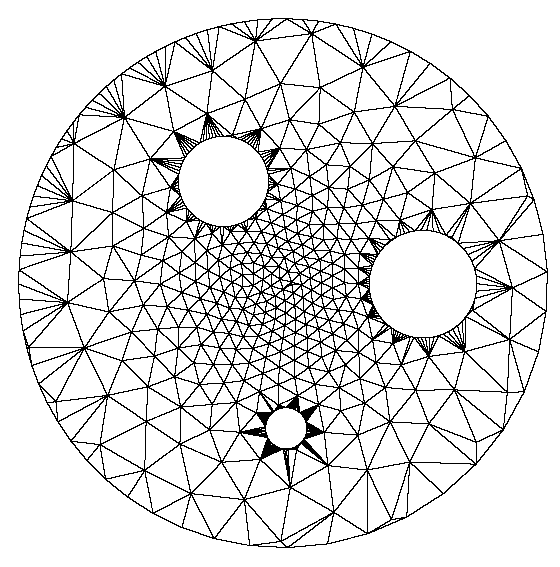
\includegraphics[width=0.4\linewidth]{image/schottky/schottky_domain2.pdf}
	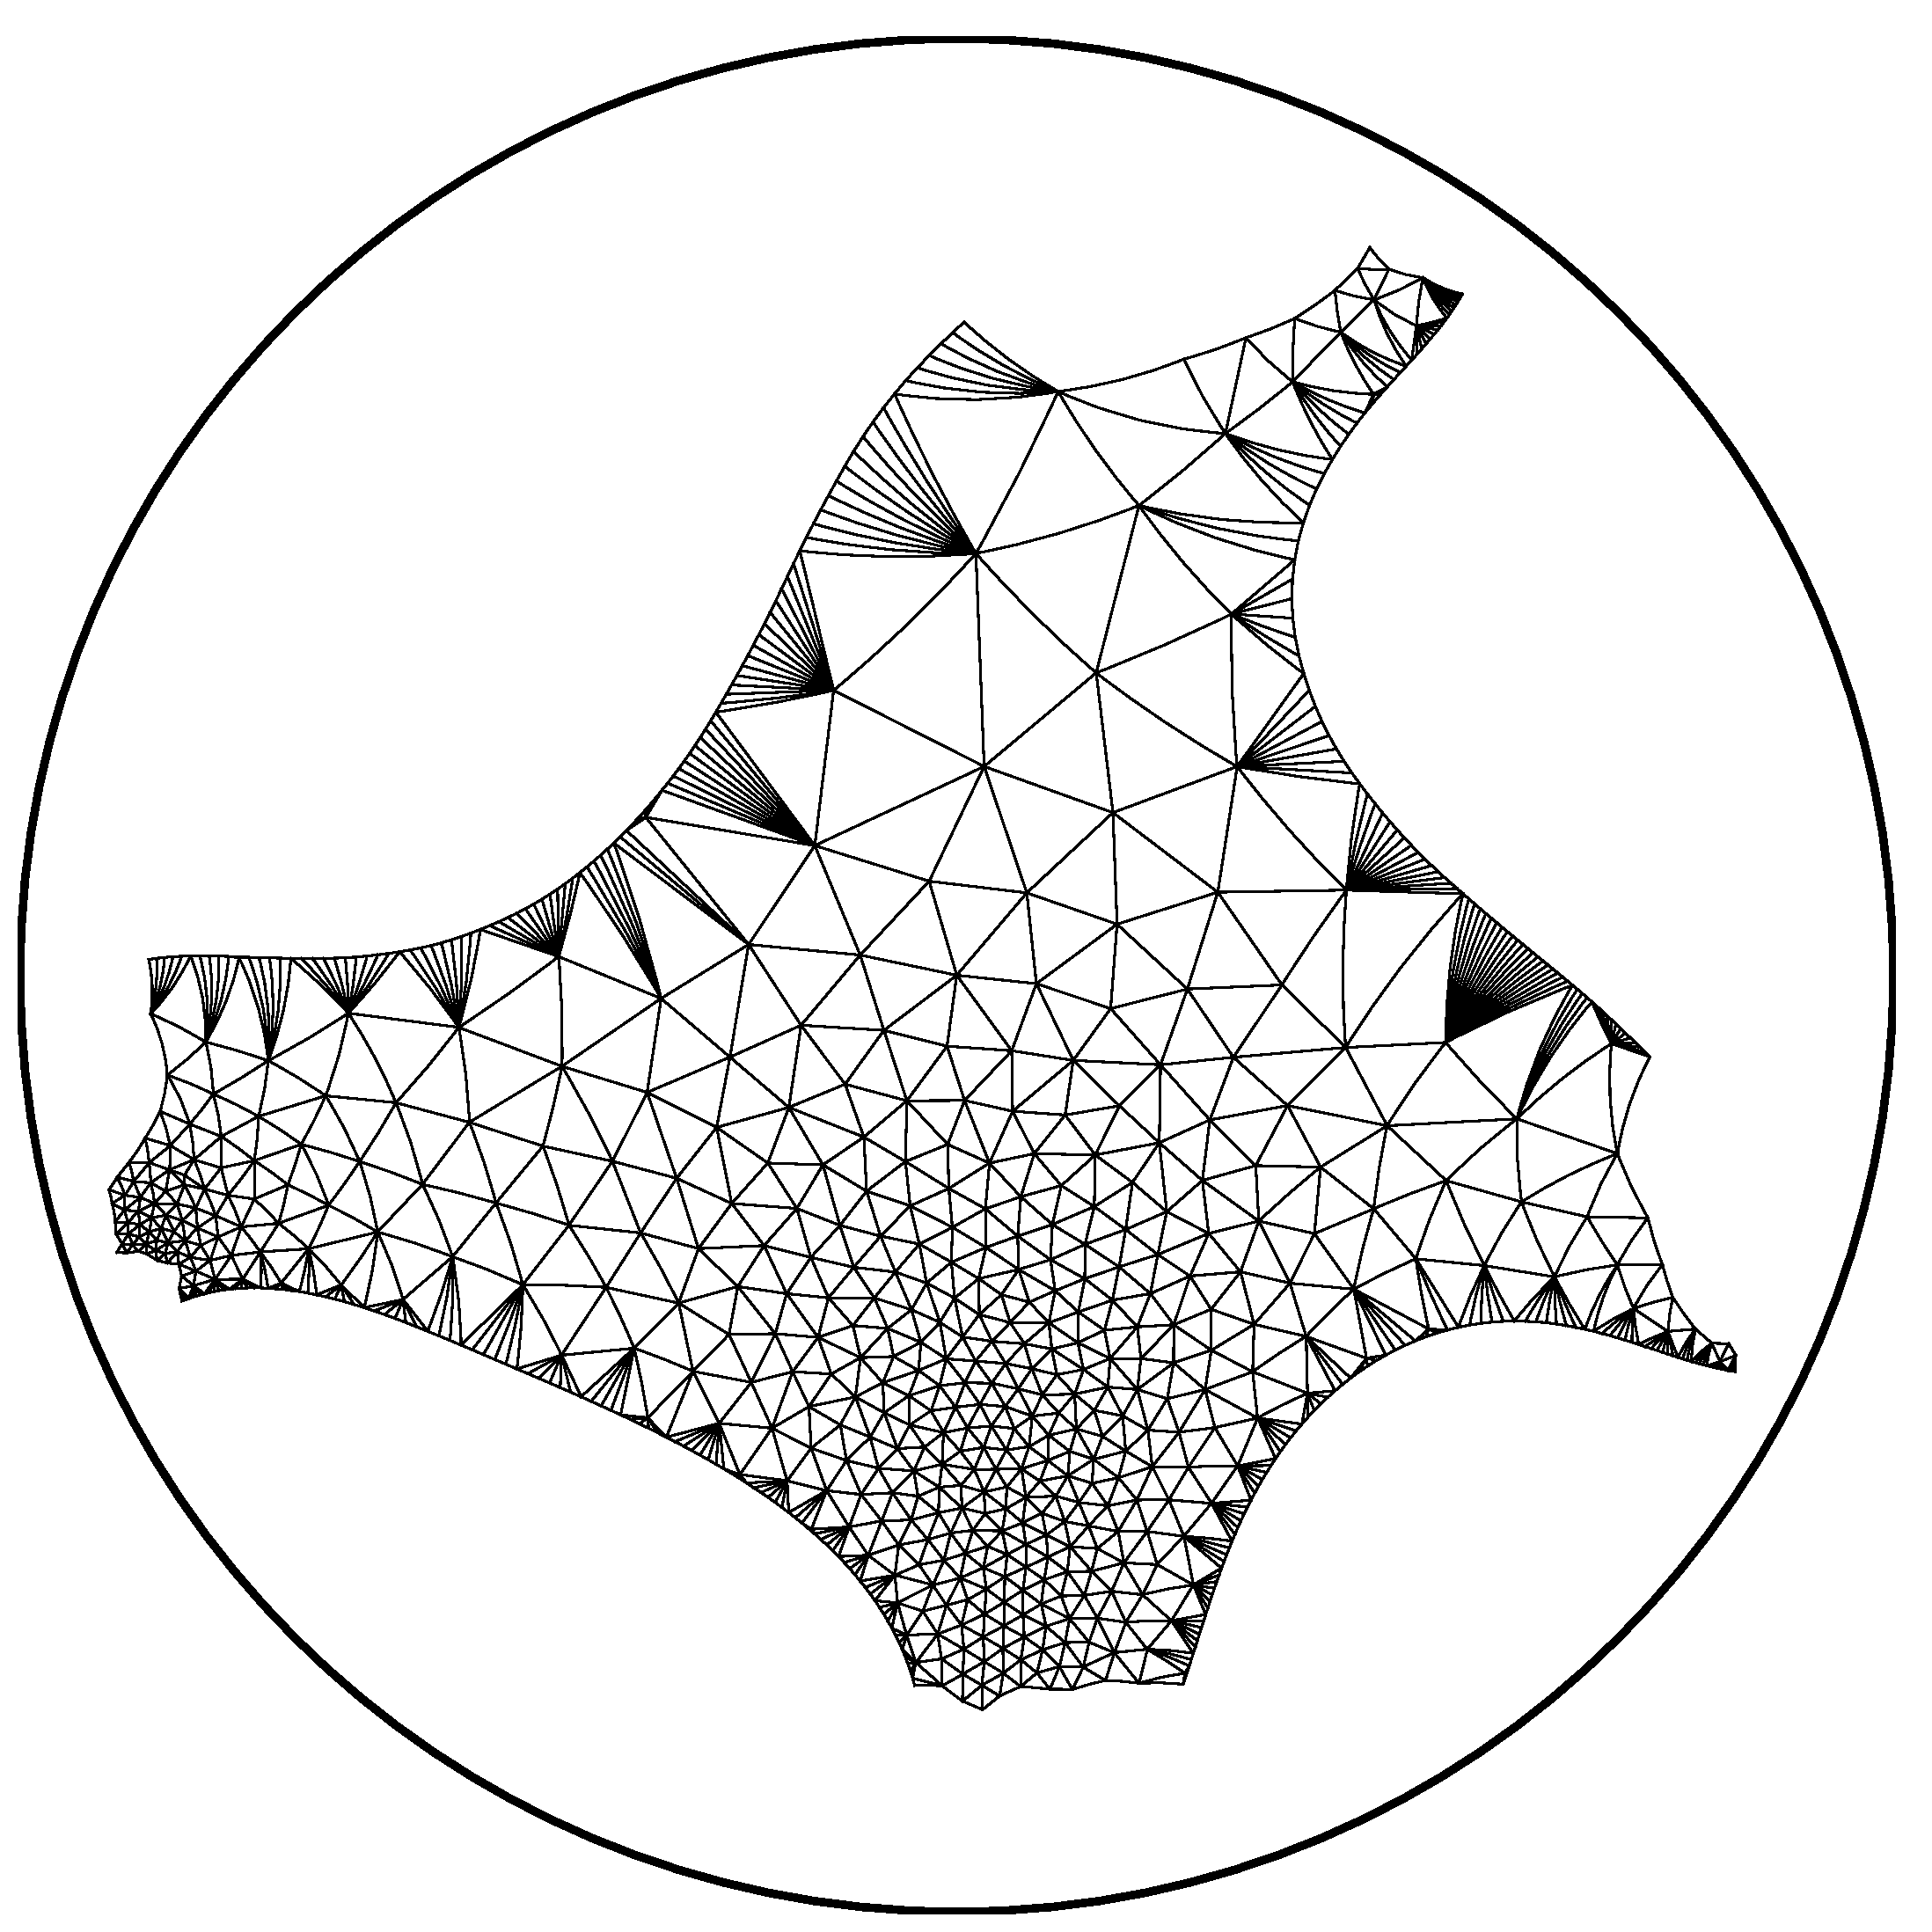
\includegraphics[width=0.4\linewidth]{image/schottky/schottky01.pdf}
	\caption{Fuchsian uniformization of a Riemann surface (right) given by Schottky data (left).}
	\label{fig:fuchsian_to_schottky}
\end{figure}

\begin{figure}
	\centering
	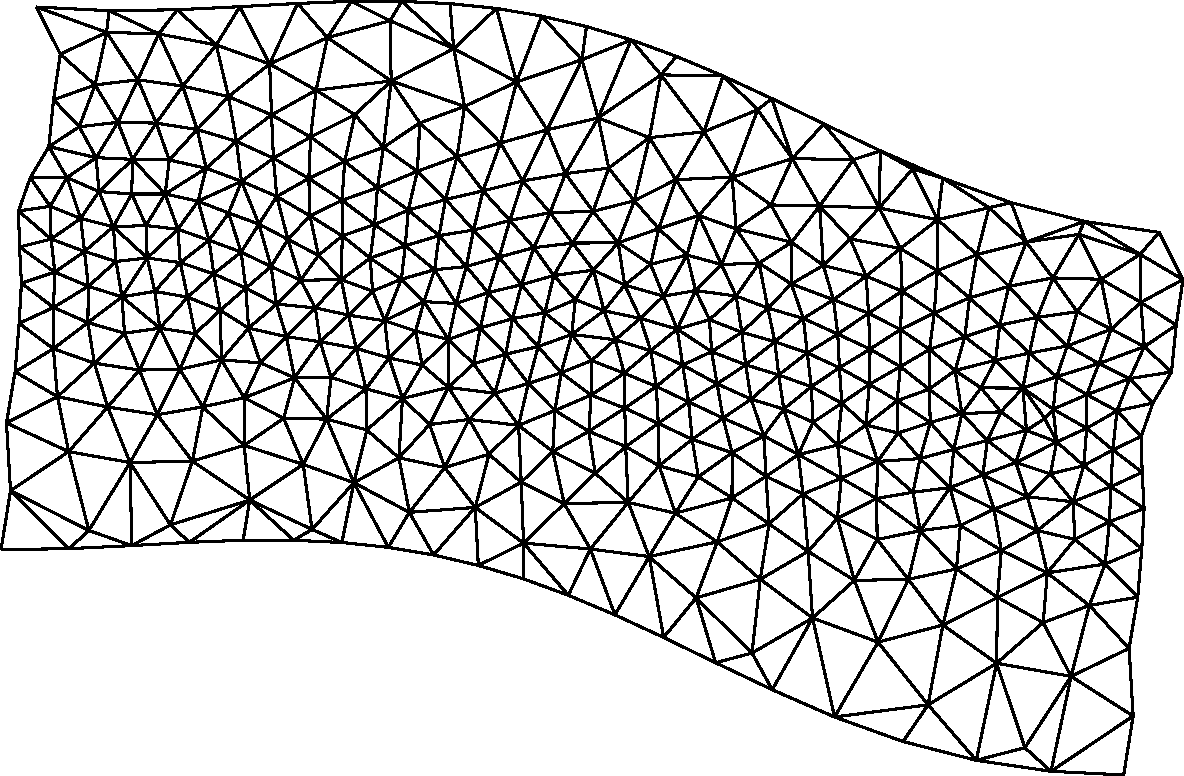
\includegraphics[width=0.4\linewidth]{image/schottky/schottky_genus1.pdf}
	\caption{Uniformization of a genus $1$ Riemann surface given by Schottky data.}
	\label{fig:fuchsian_to_schottky_genus_1}
\end{figure}

In this section we show how to use the discrete theory to calculate a Fuchsian uniformization of a Riemann surface 
given by Schottky data. For a triangulated fundametal domain of a Schottky group we show how to obtain a discretely
conformally equivalent triangulation either in the unit disk for genus greater that $1$ or in $\C$, see Figure~\ref{fig:fuchsian_to_schottky}. These triangulations build
a fundamental domain for the corresponding uniformizing Fuchsian or translation group of the given Riemann surface. We only consider classical Schottky groups here.

Let $C_1,C'_1\ldots,C_g,C'_g$ be disjoint circles in $\hat{\C}$. 
\begin{definition}
A classical Schottky group $G$ is a Kleinian group
with generators $\sigma_1,\ldots,\sigma_g$ satisfying
\[\frac{\sigma_i z - B_i}{\sigma_i z - A_i} = \mu_i \frac{z - B_i}{z - A_i}, \quad\quad\quad 0 < \left|\mu_i\right|<1,\]
where $\sigma_i$ maps the exterior of $C_i$ onto the interior of $C'_i$. The points $A_i$ and $B_i$ lie inside the circles $C_i$ and $C'_i$ respectively \cite{bobenko2011riemann}. 
\end{definition}
Figure~\ref{fig:schottky_group} illustrates this construction.
The quotient space $\Chat/G$ is a Riemann surface of genus $g$. The group $G$ is called the uniformizing
Schottky group. The points $A_i,\ldots,A_g$ and $B_i,\ldots,B_g$ are fixed points of this map.
A generator $\sigma_i$ is a M{\"o}bius loxodromic transformation with matrix representation 
\[
\begin{pmatrix}a & b\\c & d\end{pmatrix} = 
\begin{pmatrix}
	a & b \\
	c & d
\end{pmatrix}
\]

\begin{figure}
	\centering
	\scalebox{1.0}{\input{figures/schottky2.pdf_t}}
	\caption{Schottky group generating a Riemann surface of genus $2$. The point at infinity is not contained in 
any of the circles. The parameters $A$ and $B$ lie inside the cirlces by definition.}
	\label{fig:schottky_group}
\end{figure}



\subsection{Discretization}
Given a Riemann surface of genus $g$ and a classical Schottky uniformization, we calculate a corresponding 
Fuchsian uniformization using discrete conformal equivalence of spherical and hyperbolic triangle meshes.
A fundamental domain of the Schottky uniformization is the Riemann sphere without the interior of the circles.
We start with a classical Schottky group $G$. Let $\sigma_1,\ldots,\sigma_g$ be the generators of $G$. We choose circles around the fixed points of the

The triangulation of a fundamental domain has to respect the mappings between the circles. Vertices on identified 
circles have to be identified as well. It is however not clear a priori what the conformal structure of a triagulated 
fundamental domain is. The edge length on identified circles differ since there is a M{\" o}bius transformation 
between them. 

The idea to define the conformal structure is to use length cross-ratios instead of edge lengths. Both definitions are equivalent and define the conformal structure of a discrete Riemann surface. So given length cross ratios on edges we can calculate representative edge lengths in the discrete conformal class of the surface and, more obvious, vice versa. On boundary edges of the fundamental domain the length cross ratios agree since length-cross ratios are M{\" o}bius invariant.




\subsection{Images of isometric circles}
\subsection{Hyperelliptic data}

\section{Conformal maps to $\Chat$}
\subsection{Selection of Branch Data}
\subsection{Examples}

\section{Surfaces with boundary}
\label{sec:surfaces_with_boundary}
\subsection{Variation of edge length}
\subsection{Examples}
\begin{figure}
\centering
\resizebox{\textwidth}{!}{
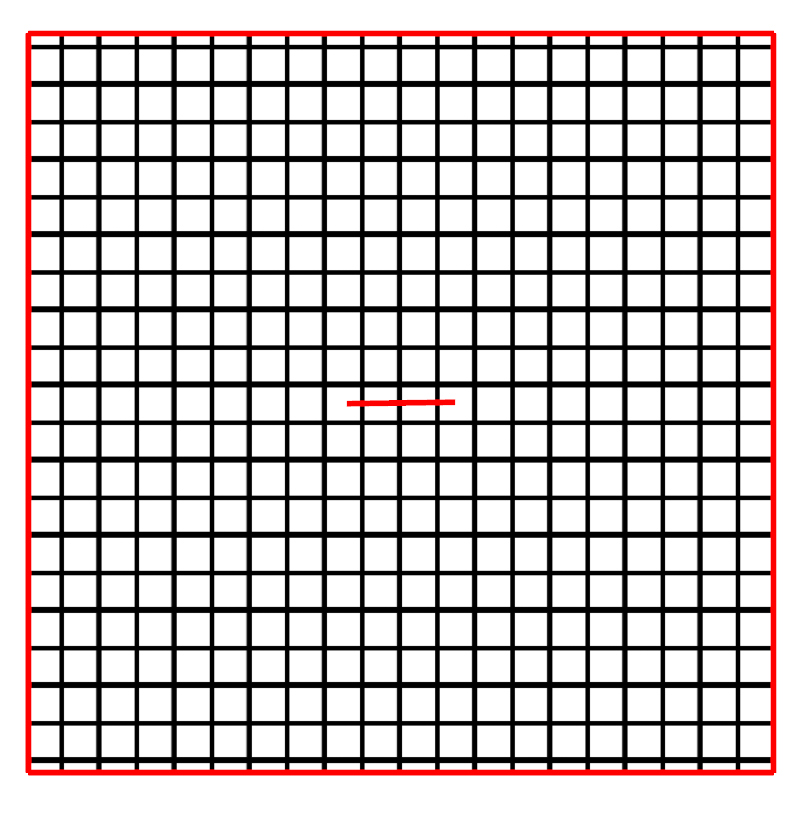
\includegraphics[width=0.5\linewidth]{image/slit_domain/domain_grid.png}
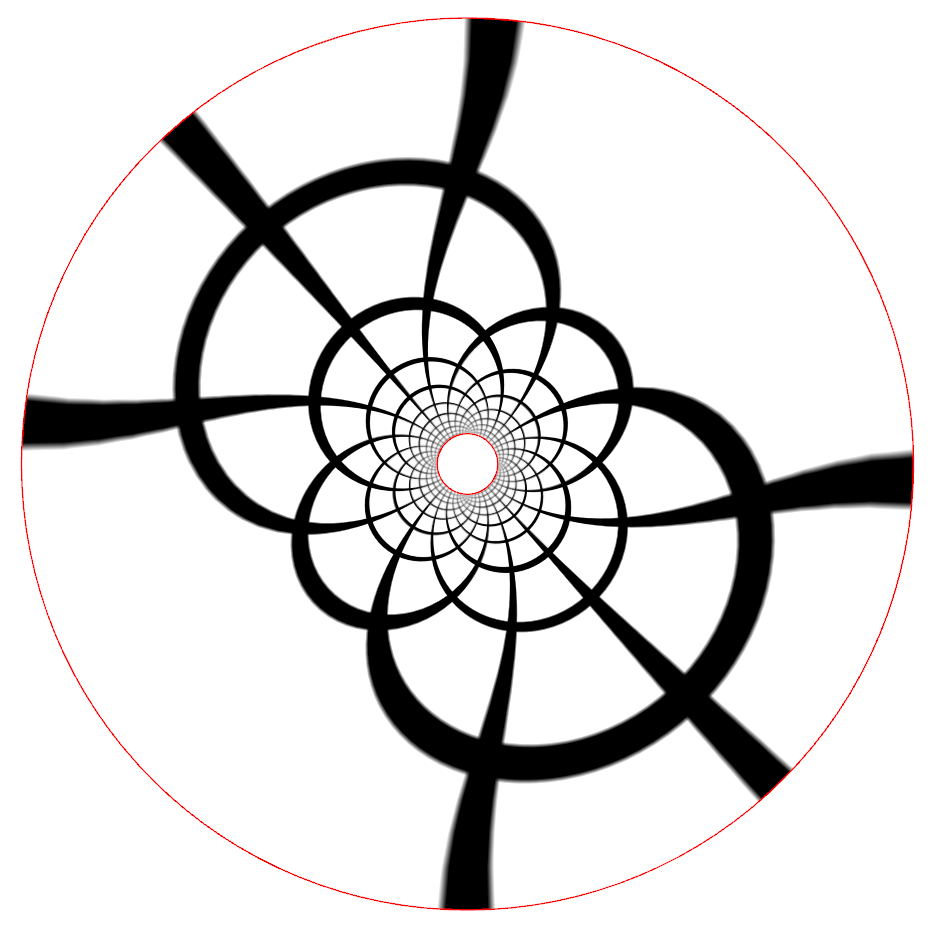
\includegraphics[width=0.5\linewidth]{image/slit_domain/image_grid.png}
}
\caption{Square with symmetric slit to the circle}
\label{fig:slit_circle}
\end{figure}


\section{Conformal maps of planar domains}
\label{sec:planar_domains}
\subsection{Boundary conditions}
\subsection{Comparison with examples of the Schwarz-Christoffel community}


%%% Local Variables:
%%% TeX-master: "Thesis.tex"
%%% End:
\part{Variational Methods for Discrete Surface Parameterization}
\documentclass[Thesis.tex]{subfiles}
\begin{document}

\chapter{Quasiisothermic mesh layout}
\label{chp:quasiisothermic}

This chapter is joint work with Thilo R{\"o}rig and Alexander Bobenko.
Most of the material presented here was published previously in the proceedings of the conference "Advances in Architectural Geometry 2012"~\cite{Sechelmann2012}. We added Section~\ref{sub:isometric} on isometric deformations of s-isothermic surfaces and Section~\ref{sec:discrete_ellipsoid} about a discrete ellipsoid.

\emph{Abstract:} 
In architecture the quality of a quad-mesh depends on the shape of the individual
quadrilaterals. The ideal shape from an architectural point of view is the
planar square or rectangles with fixed aspect ratio. A parameterization that divides a
surface into such shapes is called isothermic, i.e., angle-preserving and
curvature-aligned. Such a parameterization exists only for the special class of
isothermic surfaces. We extend this notion and introduce quasiisothermic
parameterizations for arbitrary triangulated  surfaces.

We describe an algorithm that creates quasiisothermic meshes.
Interestingly many surfaces appearing in architecture are close to
isothermic surfaces, namely those coming from form finding methods and physical
simulation. For those surfaces our method works particularly well and gives a
high quality and robust mesh layout. We show how to optimize such meshes
further to obtain disk packing representations. The quadrilaterals of these
meshes are planar and possess touching incircles.

\begin{figure}
\centering
\resizebox{\textwidth}{!}{
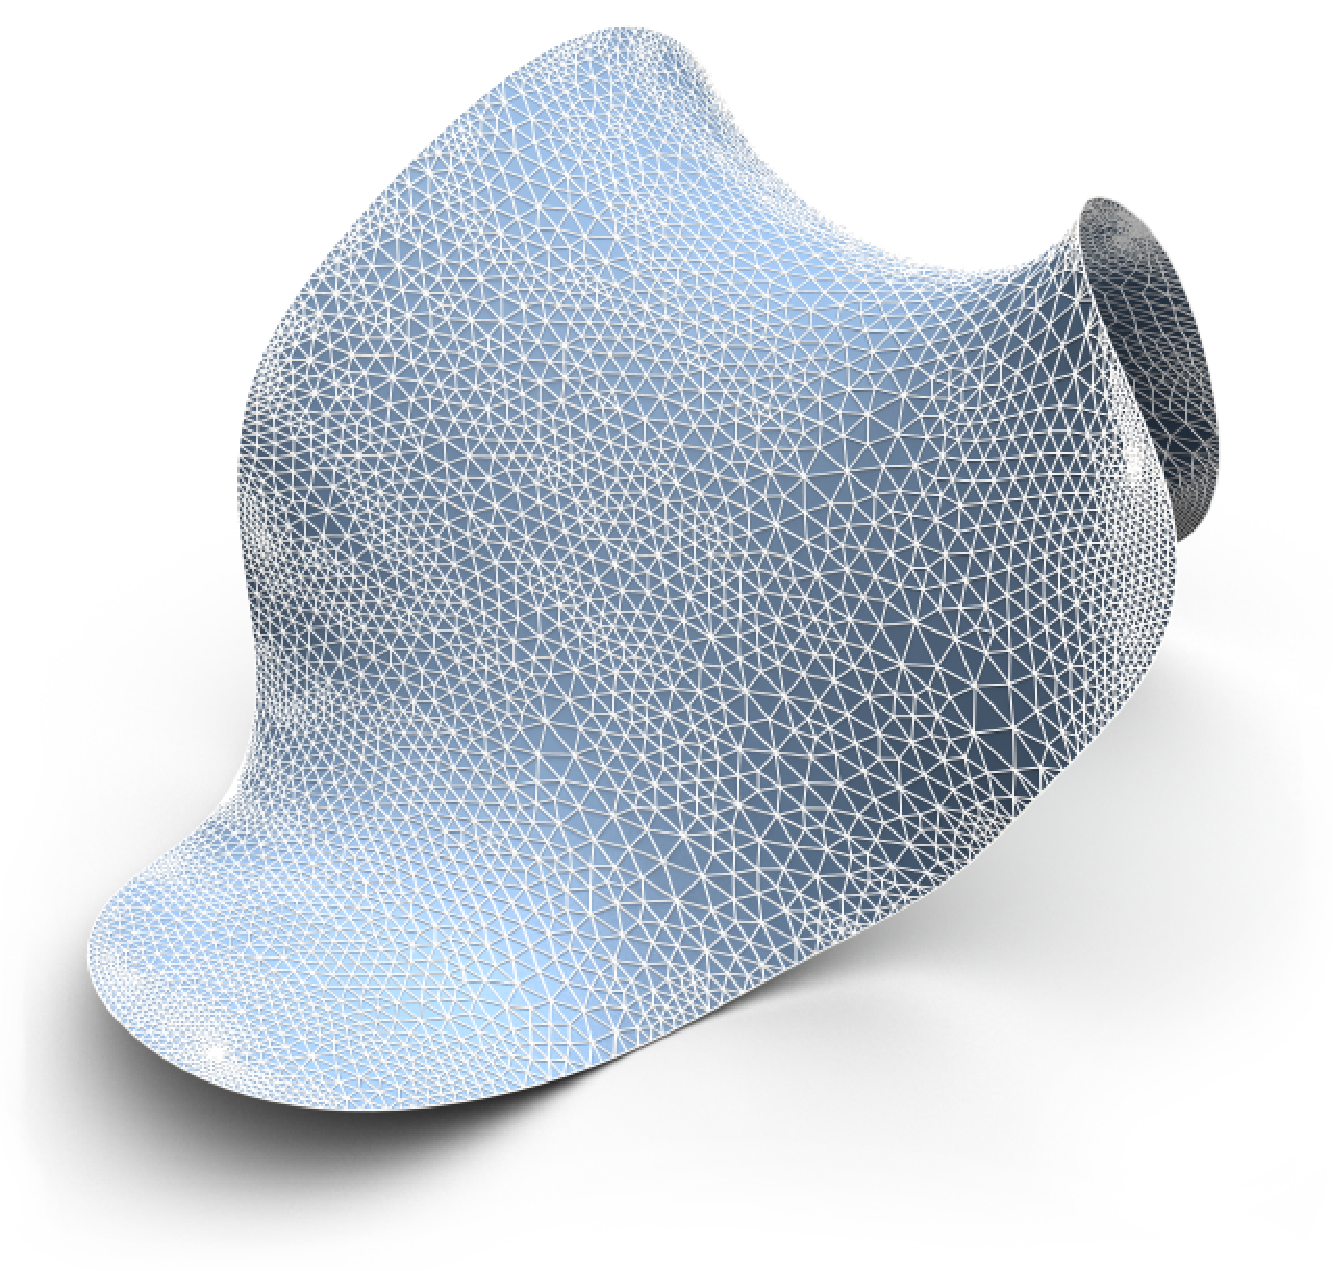
\includegraphics[width=0.48\linewidth]{image/aag2012/cover01.pdf}
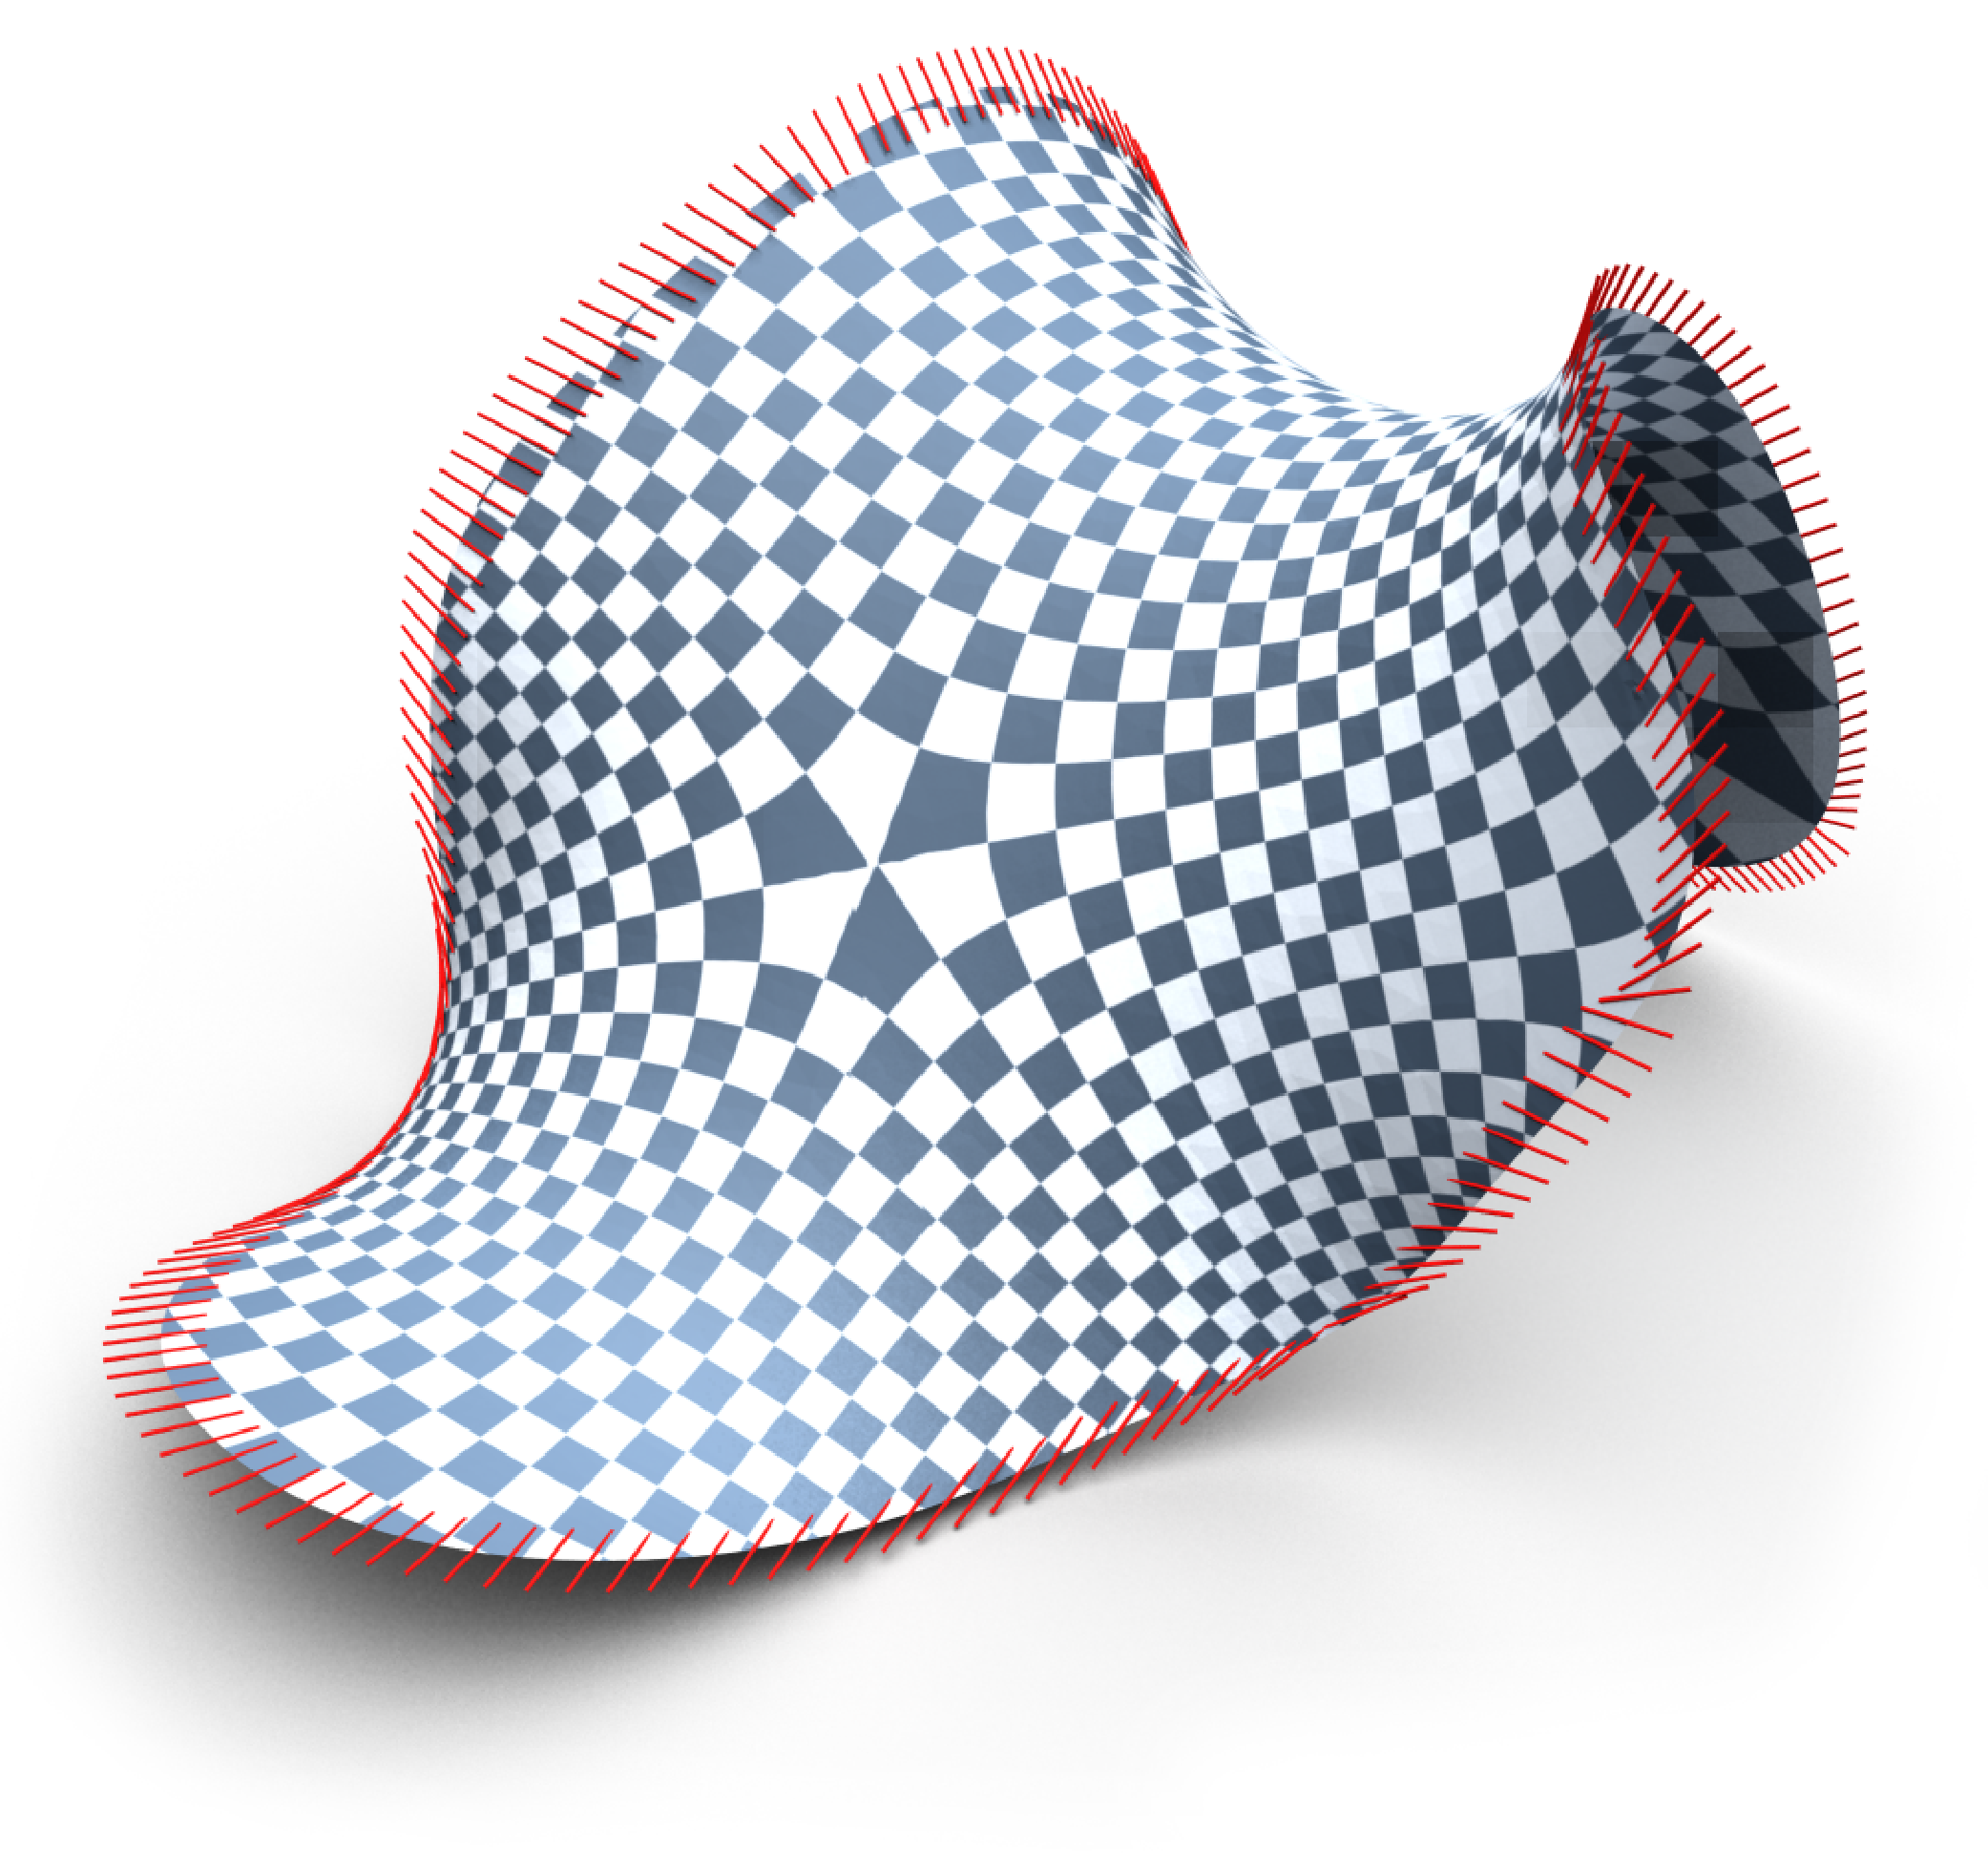
\includegraphics[width=0.48\linewidth]{image/aag2012/cover02.pdf}
}\\
\resizebox{\textwidth}{!}{
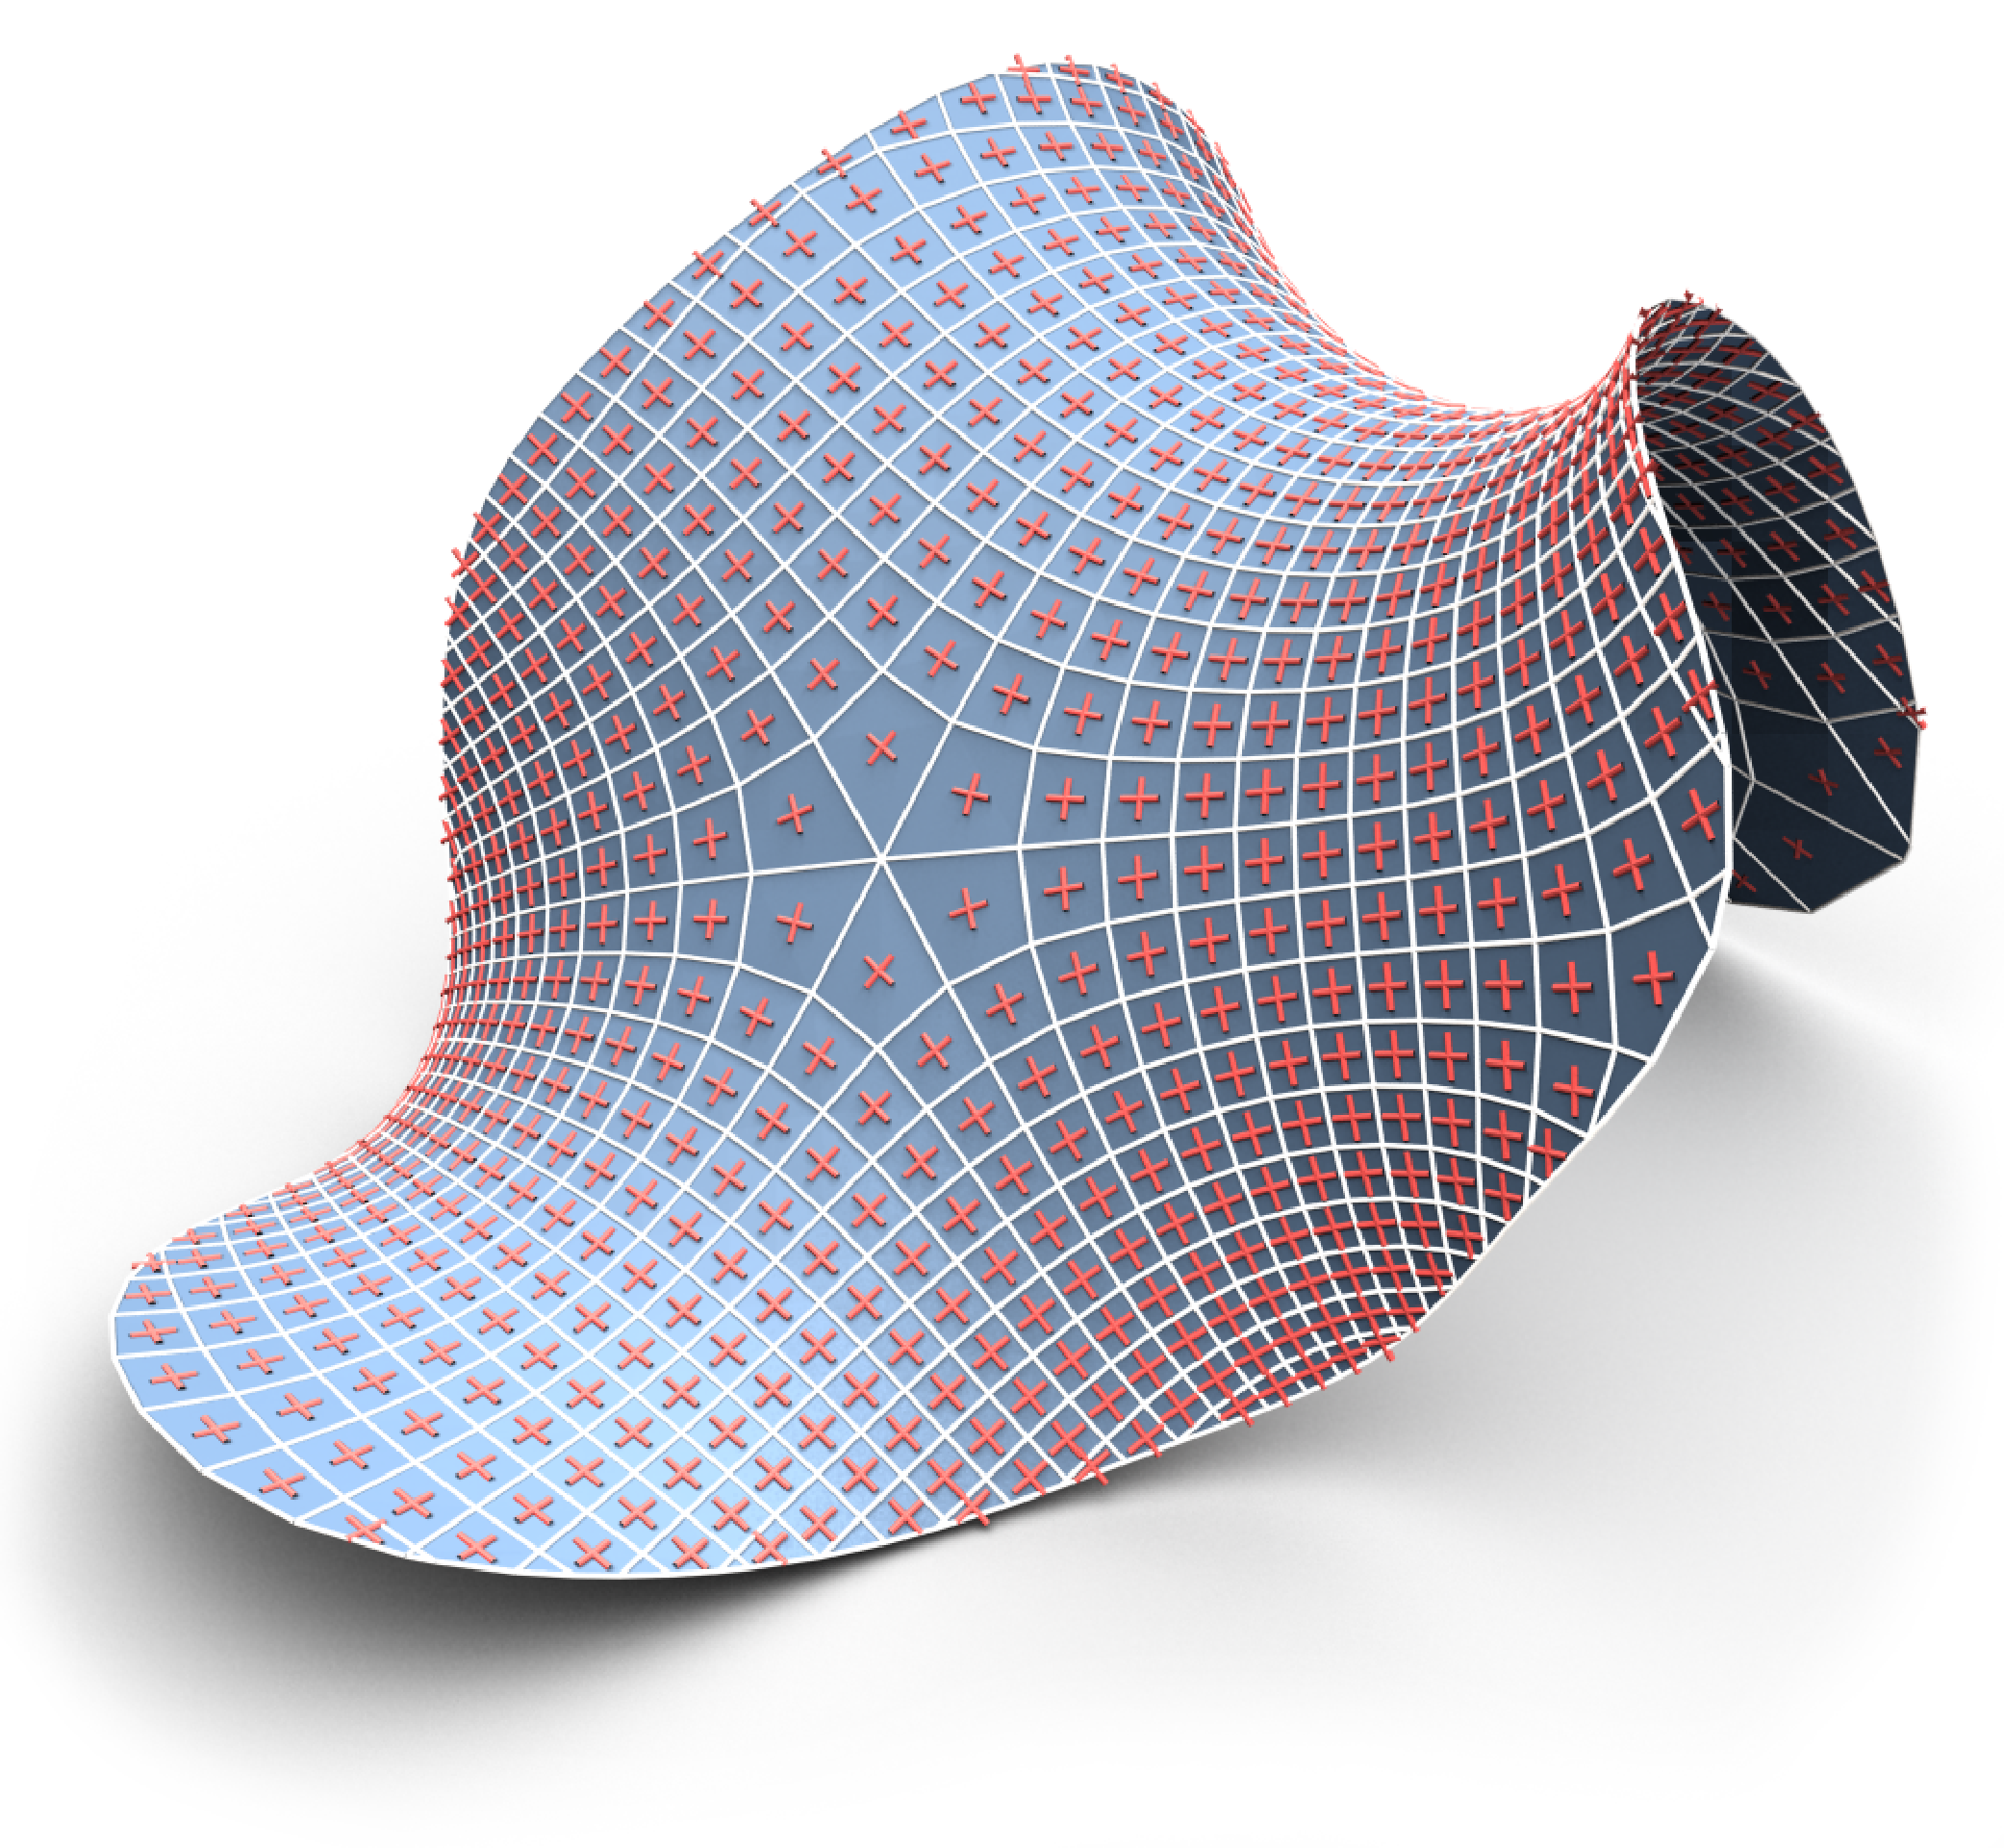
\includegraphics[width=0.48\linewidth]{image/aag2012/cover03.pdf}
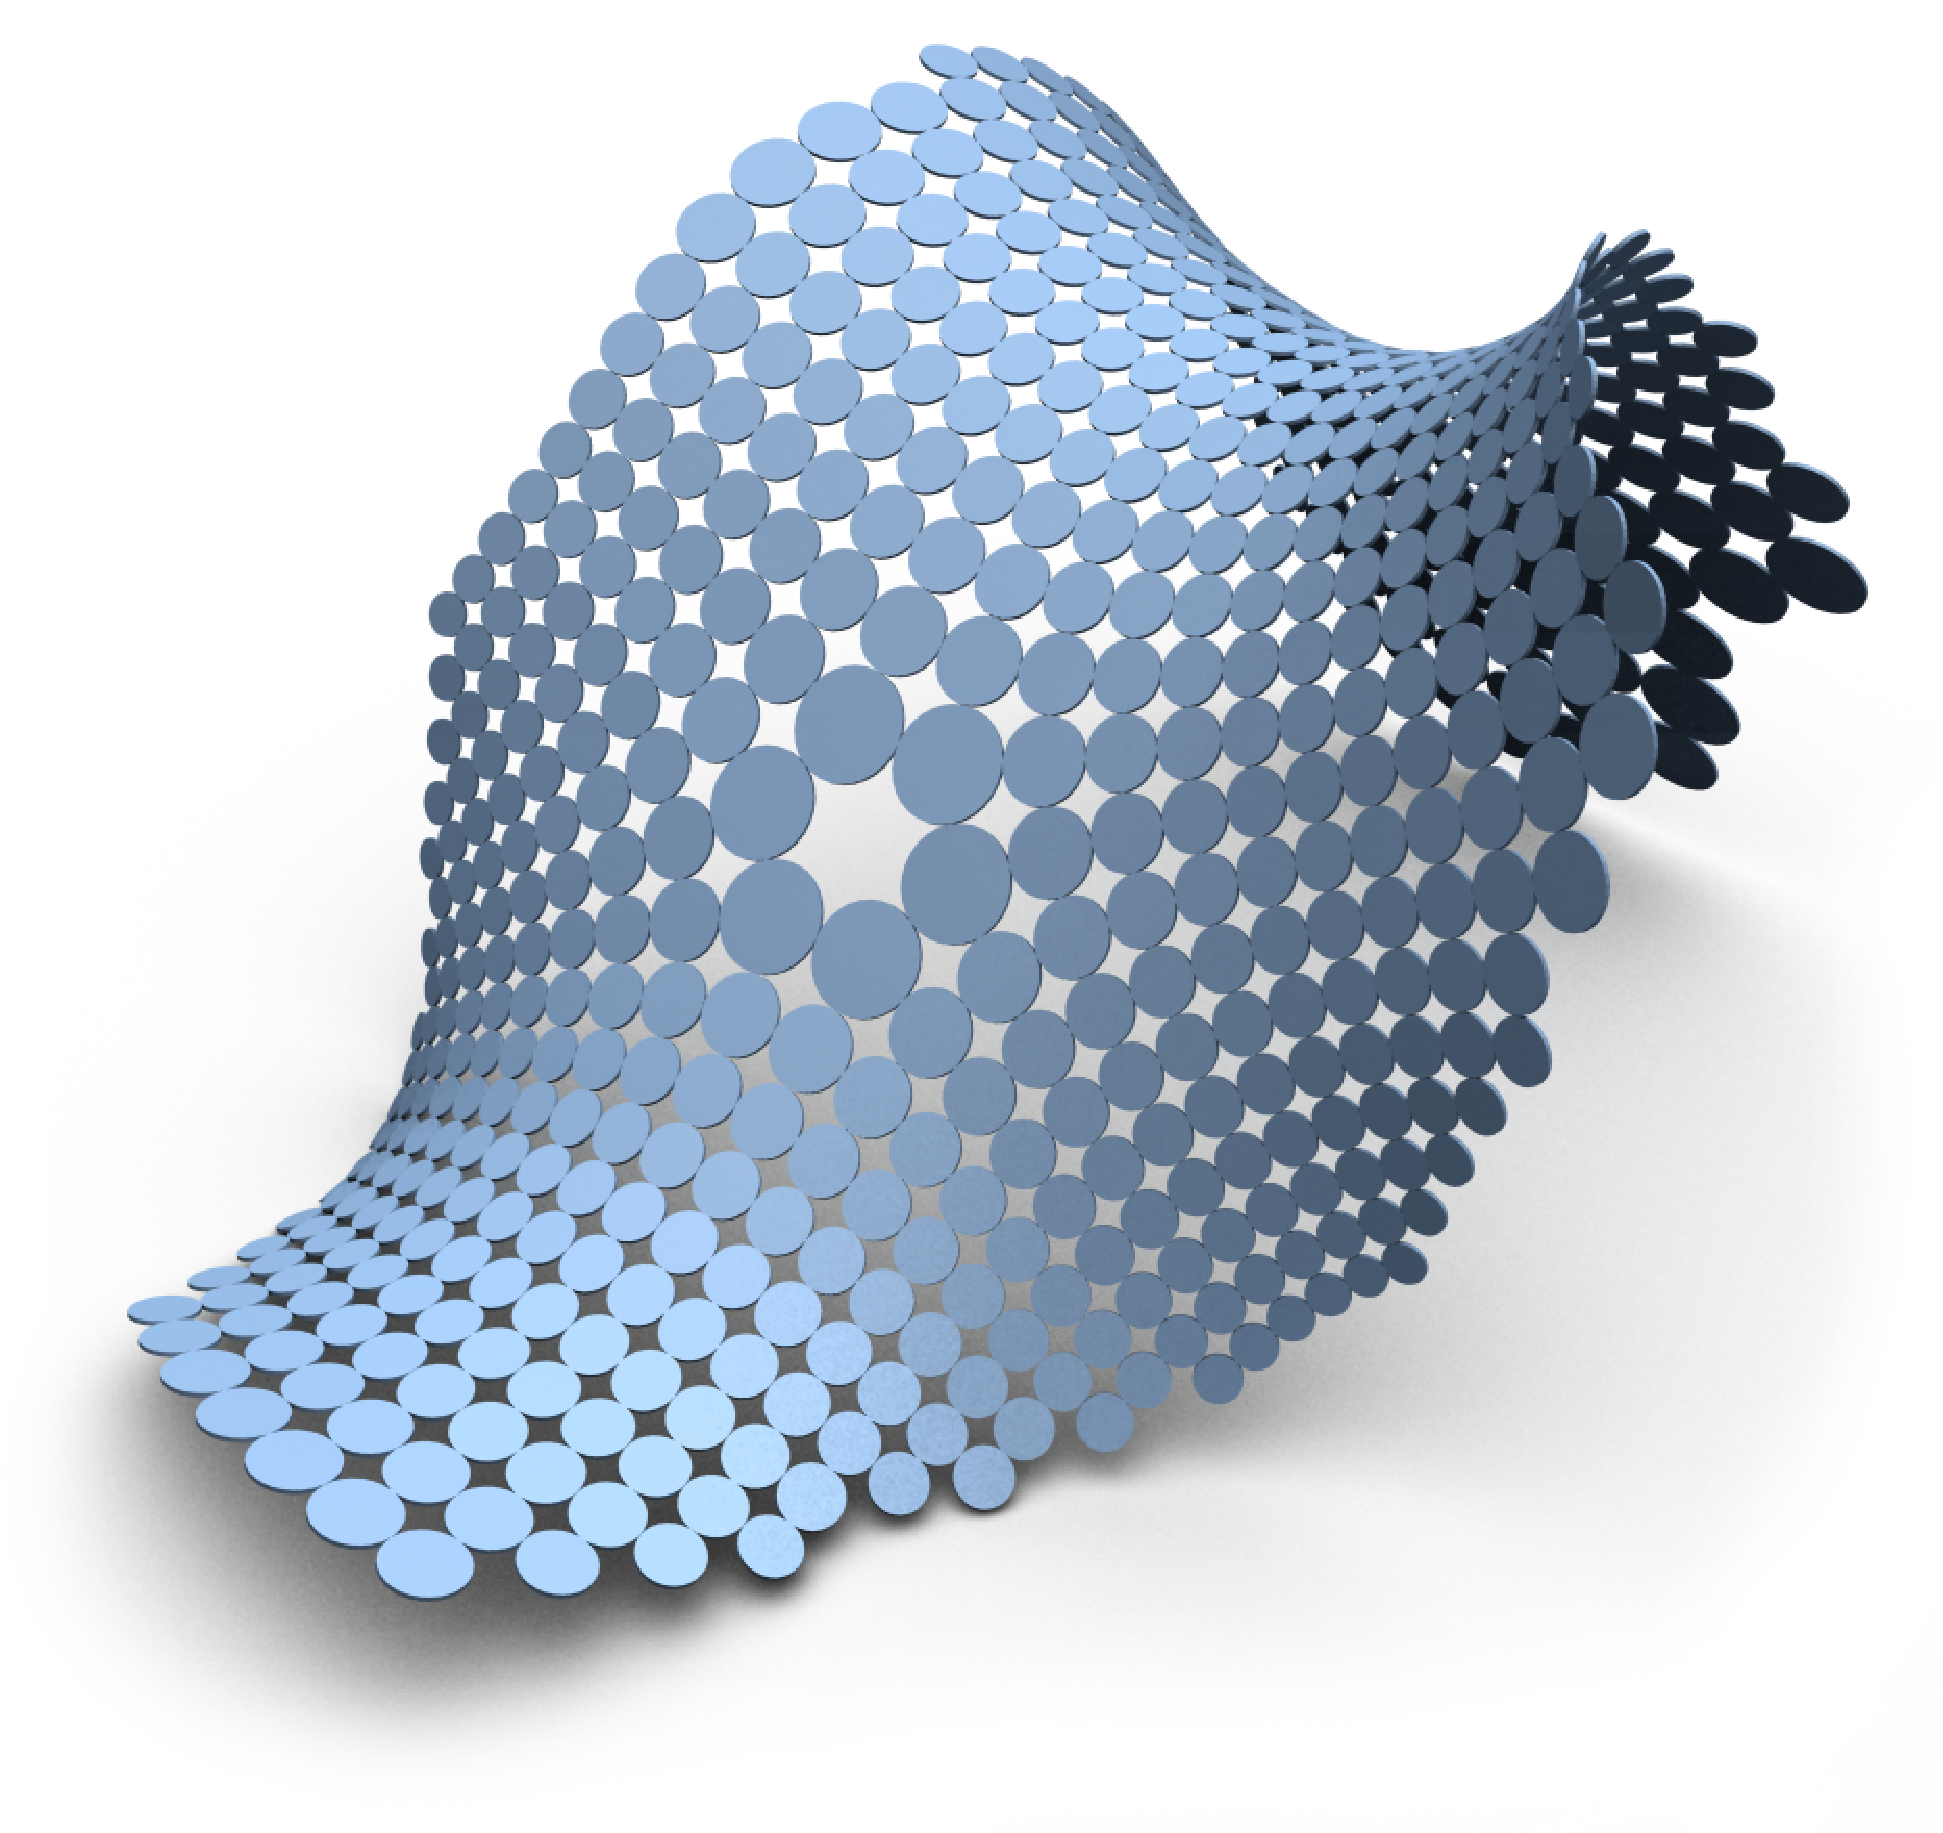
\includegraphics[width=0.48\linewidth]{image/aag2012/cover04.pdf}
}
\caption[Quasiisothermic parameterization step-by-step]{The algorithmic 
steps of this paper: For a triangulated surface we calculate 
texture coordinates by solving a boundary value problem for
principle curvature directions on boundary edges (checker board texture
and red directions). The edges of the corresponding quad mesh
align with the curvature directions (red crosses). The mesh is then
optimized towards planar quads with touching incircles.
}
\label{fig:teaser}
\end{figure}


\begin{figure}
\centering
\resizebox{\linewidth}{!}{\input{figures/all_mesh.pdf_t}}
\caption[Quasiisothermic parameterization: Examples]{The surface examples of this paper. All have been parameterized and
remeshed. $(a)$ The \textsc{Teaser} surface is the minimizer of a spring energy
with a smooth fixed boundary curve. $(b)$ A \textsc{Minimal} surface with
polygonal boundary curve. $(c)$ \textsc{Dome}: Part of a NURBS surface
exhibiting positive curvature and two curvature field singularities. $(d)$
\textsc{Roof} structure with planar boundary curve and regions of positive and
negative curvature.} 
\label{fig:all_mesh}
\end{figure}

\section{Introduction}
A key problem in architectural geometry is to convert surfaces created by form
finding methods, physical simulation, or manual modeling to quadrilateral
meshes, which are preferred for glass-steel structures. There are many 
possible quad-meshes that approximate a given shape and we study those that consist
of principle-curvature-aligned conformal squares, see Figure~\ref{fig:all_mesh}. 
Not all surface shapes can be approximated by such meshes. A smooth analog of
a surface with this property is called an isothermic surface. These surfaces admit conformal
curvature line parameterizations, i.e., angle-preserving parameterizations
aligned with the principle curvature directions. Their discrete counterpart are 
so-called s-isothermic meshes. These meshes have the additional property that
neighboring quadrilaterals possess touching incircles, see
Figure~\ref{fig:s_isothermic}.

The class of isothermic surfaces comprises, for example, constant mean
curvature surfaces. Roofs that act shell-like turn out to have almost constant
mean curvature. These are the kinds of surfaces that initiated our study of
conformal curvature line parameterizations in the architectural context. Both
conformality and alignment with curvature lines are favorable
properties for meshes. 

\noindent The contributions of this paper are:\\
\noindent\textbf{Definition of quasiisothermic parameterizations:} 
We propose a definition of quasiisothermic parameterizations of triangle meshes. 
It is based on angles between curvature directions and edges of a triangle mesh.
We define the quasiisothermic modulus that measures how isothermic a 
parameterization is. If this modulus is zero we obtain discrete isothermic 
parameterizations in the sense of our definition.

\noindent\textbf{Parameterization Algorithm:}
We give an algorithm that creates quasiisothermic parameterizations based on discrete
conformal maps of triangle meshes to the plane. This approach is built on top 
of the conformal mapping technique of Springborn~{\it et al.}~\cite{Springborn2008}. We
inherit the speed and superior projective mapping properties of their 
parameterizations.

\noindent\textbf{Variational principle for circle packing quad-meshes:}
The obtained parameterizations are used for remeshing and we optimize 
quadrilaterals to have touching incircles by minimizing a novel energy. These
s-isothermic meshes have been studied in discrete differential geometry and
possess some remarkable properties, e.g.,\ minimal s-isothermic surfaces may be
deformed isometrically retaining the same Gau{\ss} map.

The rest of the paper is organized as follows: Section~\ref{sec:previouswork}
gives an overview of existing parameterization schemes and their relation to
our approach. We also give reference to the related mathematical literature in
discrete differential geometry. In Section~\ref{sec:parametrization} we define
quasiisothermic parameterizations and a corresponding quality measure. 
In Section~\ref{sec:algorithm} we describe an algorithm to
obtain quasiisothermic parameterizations with small modulus. We describe the 
connection to discrete conformal maps and discuss how we deal with singularities. %XXX
A variational principle to generate s-isothermic meshes is presented in
Section~\ref{sec:s-isothermic}. At the end of the section we show the effect of
our optimization on several examples from different classes of surfaces. In the
final Section~\ref{sec:future} we sum up the results and propose extensions and
enhancements subject to further research.


\section{Related work}
\label{sec:previouswork}

There has been considerable work on conformal parameterizations as well as on
curvature line parameterizations related to our quasiisothermic scheme. We can 
only give a selection of previous work here.
% general parameterization 
For a general background on mesh parameterization we refer to the surveys by
Floater and Hormann~\cite{Floater2005} and Sheffer~\emph{et~al.}~\cite{ShefferPR2006}.

% conformal 
Our algorithmic approach is based on the discrete conformal equivalence of
triangle meshes as introduced by Springborn~\emph{et~al.}~\cite{Springborn2008} (see the work of
Bobenko~\emph{et~al.}\ for the mathematical background~\cite{BPS2015:dconf}). The
convex functional optimized by Springborn~\emph{et~al.}\ constructs a conformally
equivalent flat mesh for specified boundary conditions and singularities. 
Our method is related to work on angle based flattening by Sheffer and de~Sturler~\cite{Sheffer2001}. They aim for conformal parameterizations 
and express this by the additional constraint, that triangle angles have to be close 
to the original ones on the surface. For discrete isothermic parameterizations 
the definitions coincide.
%A different approach based on circle patterns is used by
%\cite{KharevychSSCircle06} to produce conformal mappings from a surface to the
%plane. Global conformal parameterizations for surfaces of arbitrary topology
%were constructed by \cite{GuYauConformal03}.

% curvature line 
Parameterizations aligning with lines of principle curvature were constructed
by Alliez~\emph{et~al.}~\cite{AlliezCDLD2003}. Their method involves 
the integration of curvature vector fields
and does not include an optimization towards conformality. 
Global parameterizations following arbitrary frame fields 
(including in particular principle curvature fields) are constructed
in the work of K\"{a}lberer~\emph{et~al.}~\cite{KalbererNP2007}. They use 
discrete Hodge decomposition and
harmonic vector fields to obtain a globally consistent parameterization. Their
QuadCover algorithm can deal with surfaces of arbitrary genus and treats
singularities using a suitable branched cover.
Both algorithms cover arbitrary triangulated surfaces and implementations are
highly complex.

% circles on surfaces 
The use of variational principles to enforce desired properties such as planarity of 
quadrilateral faces has been successfully used in architectural geometry.
Liu~\emph{et~al.}~\cite{LiuPWYW2006} propose an algorithm to optimize a quadrilateral mesh to
become planar and even conical. Pottmann~\emph{et~al.}~\cite{PottmannSBSWBW2008} use functionals to
approximate freeform surfaces with single curved panels. The energy minimized in
Section~\ref{sec:s-isothermic} is a combination of a new functional with an
energy recently described by Schiftner~\emph{et~al.}~\cite{SchiftnerHWP2009}. They construct circle
packing triangle meshes that approximate a given surface by minimizing a
combination of energies. 

Discrete s-isothermic minimal surfaces are defined in
terms of their Gau{\ss} map by Bobenko~\emph{et~al.}~\cite{BobHofSpr06}. 
This Gau{\ss} map is a Koebe
polyhedron with edges tangent to a sphere. These Koebe polyhedra also occur in
the study of edge offset meshes by Pottmann~\emph{et~al.}~\cite{PottmannLWB2007}, 
who again use a
variational approach to obtain support structures. Another parametrization
technique creating quad-dominant meshes guided by conjugate parameter
directions is given by Zadravec~\emph{et~al.}~\cite{ZadravecSW2010}. Their algorithm 
includes a level
set approach to circumvent the integration of a vector field.

The notion of discrete s-isothermic meshes was introduced in the mathematical
context by Bobenko and Pinkall as a special class of quad meshes~\cite{BobenkoP1996}.
The mathematical theory of these meshes has since then been an active field of
research in discrete differential geometry. A good overview of the recent
development and literature can be found in the book by Bobenko and Suris~\cite{BobenkoSuris2008}. 


\section{Discrete quasiisothermic parameterization}
\label{sec:parametrization}
In this section we introduce the notion of quasiisothermic parameterizations and the
corresponding quality measure.

\subsubsection{Discrete parameterizations}
Let $M=(V,E,F)$ be a triangle mesh. The elements of $V$ are the vertices of the
mesh denoted by simple indices $i\in V$. Edges are denoted by double
indices $\mathrm{\it{ij}}\in E$, and faces are denoted $\mathrm{\it{ijk}}\in F$. A triangulated surface is
a map $S:V\to \mathbb R^3$, $i \mapsto (x_i, y_i, z_i)$.
We call a map $\Phi: V \to \mathbb R^2$, $i \mapsto (u_i,v_i)$ a \emph{discrete
parameterization} of the surface $S$. We only consider orientable surfaces and
parameterizations that preserve the orientation of the triangles with respect to
the canonical orientation of $\mathbb R^2$. 

The next definition connects arbitrary parameterizations with certain directions
tangent to the surface $S$, e.g., curvature directions. Such a direction is encoded as 
an angle per edge. 
%XXX: Ueberleitung; discrete $\alpha$-parameterization? 
% definition parameterization with \alpha
\begin{definition}
Let $\alpha : E \to ]-\frac{\pi}{2},\frac{\pi}{2}]$, $\mathrm{\it{ij}} \mapsto \alpha_{\mathrm{\it{ij}}}$
be a map that assigns an angle to each edge. A discrete parameterization 
$\Phi: V\to \mathbb R^2$, $i \mapsto (u_i,v_i)$ is called a \emph{discrete
parameterization with $\alpha$} if
\begin{equation}
\label{eq:isothermic}
\tan \alpha_{\mathrm{\it{ij}}} = \frac{u_i - u_j}{v_i - v_j}
\end{equation}
for all edges of the mesh.
\end{definition}
In other words, in a parameterization with $\alpha$ the image of an edge $\mathrm{\it{ij}}\in
E$ under the map $\Phi$ encloses the prescribed angle $\alpha_{\mathrm{\it{ij}}}$ with the
$v$-axis of the parameter space. One could equally use the $u$-axis here.

\begin{figure}
\centering
\resizebox{\textwidth}{!}{\input{figures/isothermic.pdf_t}}
\caption{A discrete isothermic parameterization. Angles between triangle edges 
and a curvature direction family are preserved by the map.}
\label{fig:isothermic_parameterization}
\end{figure}

\subsubsection{Quasiisothermic parameterizations}
Our main example of a parameterization with an angle function $\alpha$ comes
from $\alpha$ defined by the curvature directions of a surface $S:V\to
\mathbb R^3$ (see Fig.~\ref{fig:isothermic_parameterization}). For a triangulated surface 
curvature directions and magnitudes can be calculated and assigned to edges. This 
is usually done by averaging curvature information over neighborhoods of points 
on the surface \cite{CohMor03}. A discrete parameterization 
with angle function $\alpha$ stemming from the curvature direction field is then called a
\emph{discrete isothermic parameterization}. Indeed, the latter is just a
curvature line parameterization. In our case the curvature directions
are mapped to the coordinate directions in the $(u,v)$-plane. The map can be
treated as conformal: Angles between edges and curvature directions are 
preserved.

Generic surfaces do not allow for isothermic parameters (those admitting
isothermic parameterizations are called isothermic surfaces). Therefore we do
not expect a parameterization with given $\alpha$ to exist in general. To be
able to deal with arbitrary surfaces we introduce the notion of discrete
quasiisothermic parameterization. The idea is to obtain a parameterization with
angles $\tilde\alpha$ as close to the curvature directions $\alpha$ as possible.
Let
\begin{equation}
Q^\alpha(\mathrm{\it{ij}})=\left|\alpha(\mathrm{\it{ij}}) - \tilde\alpha(\mathrm{\it{ij}})\right|
\label{eq:quasiisothermicity}
\end{equation}
where $\tilde\alpha(\mathrm{\it{ij}})$ is angle the between the $v$-axis and the edge $\mathrm{\it{ij}}$ in 
parameter space.
\begin{definition}
We call a discrete parameterization $\Phi$ with angle function $\alpha$ 
\emph{quasiisothermic} with modulus $Q\in \mathbb R_+$ if
\begin{equation}
Q^\alpha(\mathrm{\it{ij}}) \leq Q
\end{equation}
for all edges $\mathrm{\it{ij}}\in E$.
\end{definition}
The motivation for this measure of quasiisothermicity is the following: If $Q$ is small
the directions of principle curvature on the surface are almost tangent to the parameter 
lines of the parameterization. For a modulus of zero we have an in a sense angle 
preserving map where edges enclose the same angles with the coordinate axes in 
parameter space as with curvature directions on the surface. We will now 
create parameterizations that have small $Q$.


\section{Minimization of the functional}
\label{sec:algorithm}

In this section the surface $M$ is a triangulated surface with one boundary
component. We will now construct a function $\Phi$ that
has zero approximation error $Q^\alpha$ at boundary edges and is a discrete
conformal map in the sense of Springborn~\emph{et~al.}~\cite{Springborn2008} in the 
interior of the
surface. We argue under which circumstances this leads to nice
behaviour in the interior. We start by briefly introducing discrete conformal
maps and the boundary conditions we need for our purposes.

\subsubsection{Discrete conformal maps}
\label{subsub:discrete_conformal_maps}

We recall the definition by Springborn~\emph{et al.} of discrete conformal 
maps via conformal equivalence of triangle meshes. It is stated in terms of
lengths of the surface edges and corresponding parameter edges in the 
$(u,v)$-plane.
\begin{definition} 
  A discrete parameterization~$\Phi$ is \emph{conformal} if there exists a
function $\mu:V \to \mathbb{R}$, $i \mapsto \mu_i$ such that the following
condition for the edge lengths $l_{\mathrm{\it{ij}}}$ on the surface and
$\tilde{l}_{\mathrm{\it{ij}}}=\Vert\Phi(i)-\Phi(j)\Vert$ in parameter space holds
\begin{eqnarray}
  \label{eq:discrete_conformal} 
  \tilde{l}_{\mathrm{\it{ij}}}=\mu_i\mu_j l_{\mathrm{\it{ij}}}.
\end{eqnarray}
\end{definition}
%XXX (u,v)-plane vs. function u
For a given triangle mesh there is a unique solution $\mu$ that retains the 
boundary edge lengths. Another unique solution can be obtained by fixing 
the angles between consecutive boundary edges. These angles have to be 
chosen consistently obeying the Gau\ss-Bonnet relation 
(see the section about singularities).

The function~$\mu$ for a given triangle mesh can be found as the minimizer 
of a convex functional. Thus its computation is efficient. The resulting 
parameterization is created by a breadth-first layout that enumerates 
all triangles and assigns texture coordinates. In addition to boundary angles 
one can ask for solutions that contain special interior vertices where the
 sum of triangle angles is not equal to $2\pi$ (see Fig.~\ref{fig:teaser}). 
These so-called cone points will be inserted at singularities of the 
parameterization.


\subsubsection{Curvature boundary conditions}
\label{subsub:boundary}

\begin{figure}
\centering 
\resizebox{\textwidth}{!}{\input{figures/boundary_conditions2_horizontal.pdf_t}}
\caption[Curvature boundary conditions]{Curvature boundary conditions: In parameter space the interior angle 
$\theta_j$ at the vertex~$\Phi(j)$ has to be chosen such that curvature 
directions given by angles $\alpha_{\mathrm{\it{ij}}}$ and $\alpha_{\mathrm{\it{jk}}}$ align with the 
$v$-axis. This choice is unique up to addition
of $k \pi$. The above pictures show two possible layouts in the parameter
plane depending on the interior angle sum on the surface.}
\label{fig:boundary_angles}
\end{figure}

Let $\alpha:E\to ]-\frac{\pi}{2},\frac{\pi}{2}]$ be an angle function derived
from numerical curvature directions and the given surface orientation. 
Let $\mathrm{\it{ij}}\in E$ and $jk\in E$ be two consecutive boundary edges with common
vertex $j$ and let $\tilde\theta_j$ be the sum of interior triangle angles on
the surface at this vertex.  The direction of the edge $\Phi(\mathrm{\it{ij}})$ (resp.\
$\Phi(\mathrm{\it{jk}})$) is determined by the angle $\alpha_{\mathrm{\it{ij}}}$ 
(resp. $\alpha_{\mathrm{\it{jk}}}$),
since the curvature directions encoded by the $\alpha$'s should align with the
$v$-axis. The orientation of the surface (resp.\ the boundary edges) defines
the angle $\theta_j$ between the edges $\Phi(\mathrm{\it{ij}})$ and $\Phi(\mathrm{\it{jk}})$ up to
addition of $k \pi$ (see Fig.~\ref{fig:boundary_angles}). To make the angle
unique we require that the difference between the original surface angle
$\tilde\theta_j$ and the angle in the parameter plane $\theta_j$ is as small
as possible, i.e.,\ choose $k>0$ as small as possible such that 
\[
|\underbrace{\angle(\Phi(\mathrm{\it{ij}}),\Phi(\mathrm{\it{jk}}))+ k \pi}_{\theta_j} - \tilde\theta_j| \le \pi/2.
\]
See Figure~\ref{fig:boundary_angles} for an
illustration of the alignment in the parameter plane. The angles $\theta_j$ at
boundary vertices serve as boundary conditions for the discrete conformal
parameterization. A conformal parameterization with these boundary conditions
will then have perfect alignment of curvature directions at the boundary.

\subsubsection{Singularities}
\label{subsub:singularities}
There exists an analog of the smooth Gau{\ss}-Bonnet theorem
for discrete surfaces that relates the Gaussian and the boundary curvature to
the Euler characteristic. During parameterization we construct a metric that is
flat everywhere except for cone singularities where positive or negative
curvatures are introduced. For the purpose of curvature line parameterizations
we can only have cone points with discrete curvatures of $\pi$, $0$, or $-k\pi$
at singularities of the curvature direction field. The Gaussian curvature
$\kappa_i$ at interior vertices~$i\in V_I$ is the angle defect, i.e., $\kappa_i =
2\pi-\theta_i$, where $\theta_i$ is the sum of the angles at the vertex~$i$.
For a boundary vertex $j\in V_B$ the corresponding geodesic curvature is defined by
$\kappa^g_j = \pi-\theta_j$. So if we split the vertex set $V = V_B \cup V_I$ into
boundary vertices $V_B$ and interior vertices $V_I$ the discrete
Gau{\ss}-Bonnet theorem becomes:
\begin{equation}
  \label{eq:gauss-bonnet} \sum_{i\in {V_I}}\kappa_i + \sum_{j\in
  V_B}\kappa^g_j = 2\pi \chi,
\end{equation} 
where $\chi$ is the Euler characteristic of the surface ($\chi = 1$ for disks).
Since all curvature directions at boundary edges in parameter space become parallel, the
boundary curvature adds up to a multiple of $\pi$. If this sum happens to
differ from $2\pi$, there must be singularities in the curvature field and we
have to compensate the deficit at interior vertices to satisfy
Equation~(\ref{eq:gauss-bonnet}). In Figure~\ref{fig:dach01_directions} the
boundary curvature sum of the domain is $4\pi$. So by inspection of the curvature field in the 
interor of the surface we picked two singularities each of curvature $-\pi$ to satisfy the 
Gau{\ss}-Bonnet equation. They correspond to cone points with angle $3\pi$ in the 
parameterization.

\begin{figure}[t]
\centering
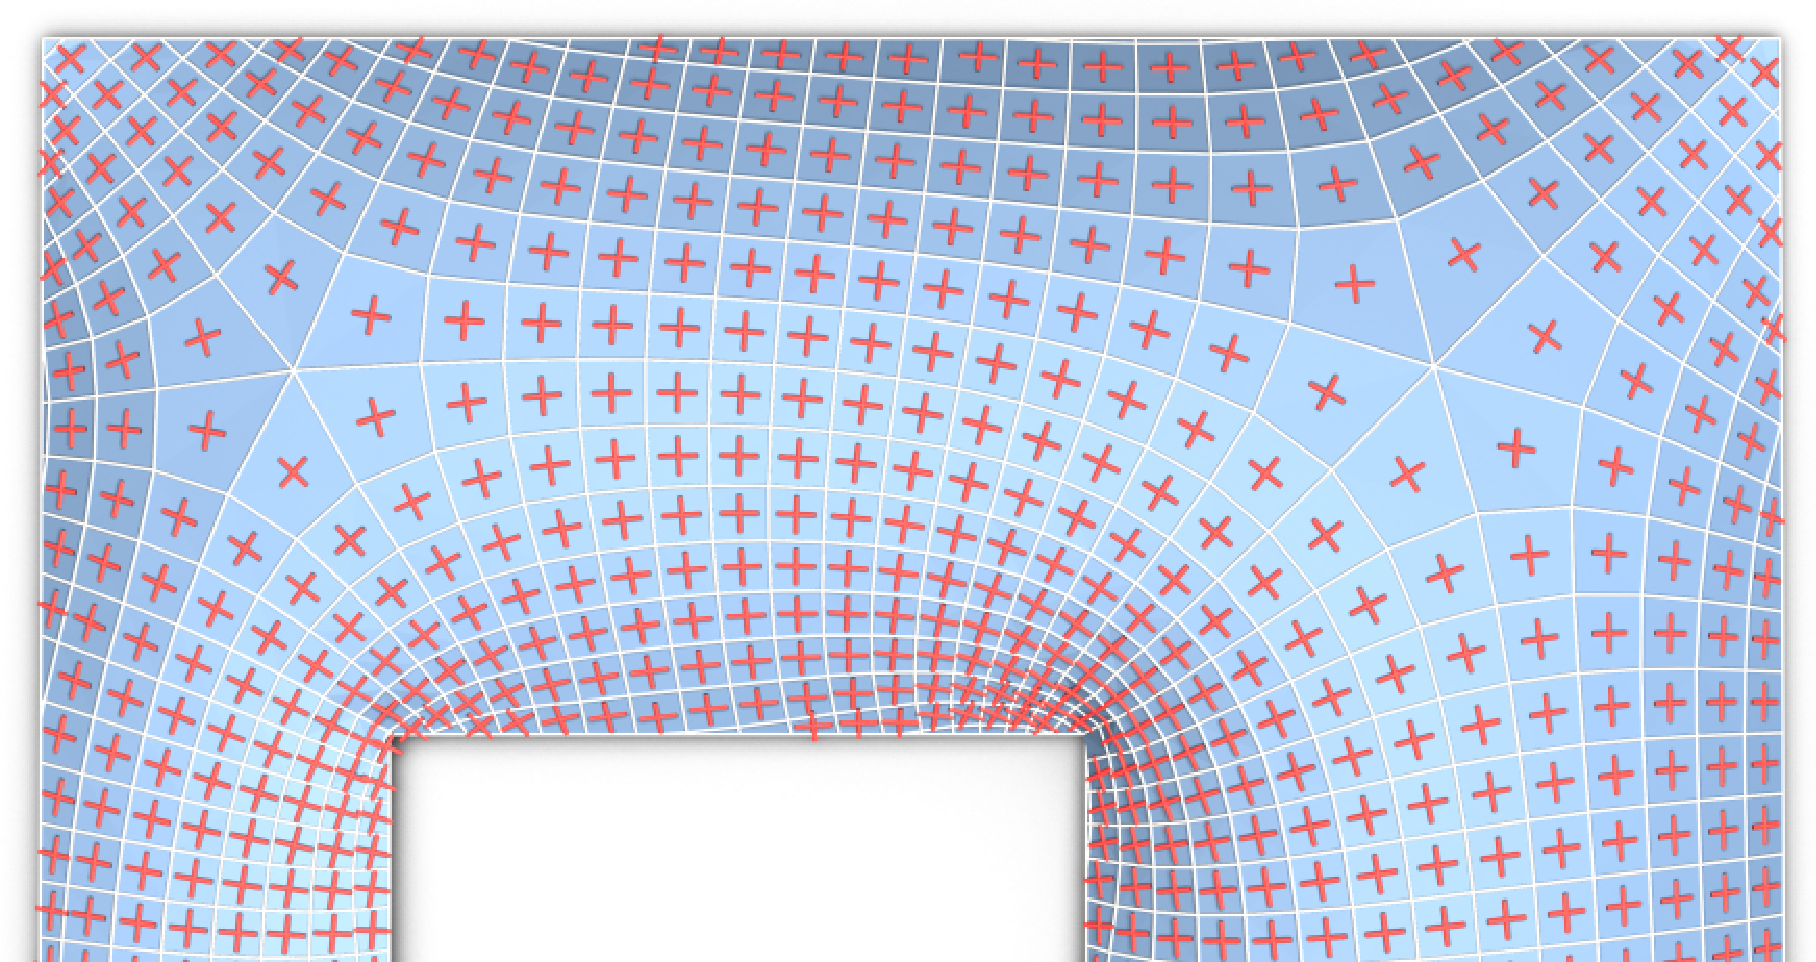
\includegraphics[width=\linewidth]{image/aag2012/dach_example01_directions.pdf}
\caption{Parameterization of the \textsc{Roof} model. The discrete 
curvature lines approximate curvature directions with high quality. See 
Section~\ref{subsub:examples_quality} for a discussion.}
\label{fig:dach01_directions}
\end{figure}

\subsubsection{Implementation}
\label{subsub:parameterization}

The algorithm to compute a quasiisothermic parameterization with vanishing modulus at the 
boundary of the domain is the following:
\begin{compactenum}[(1)]
\item Generate curvature directions and compute $\alpha$ at the boundary
\item Calculate boundary angles $\theta$ and pick singularities
\item Compute conformal parameterization with given $\theta$s
\item Perform remeshing
\item Remove cone point cuts 
\end{compactenum}

To estimate principle curvature fields we use the method of Cohen-Steiner and
Morvan \cite{CohMor03}, where the curvature tensor is averaged over a disk of a
given radius centered at edge midpoints. Together with a fixed orientation
of the surface this defines the angle function
$\alpha$. 

We deduce the angles $\theta$ for the boundary vertices as described in
Section~\ref{subsub:boundary}. These angles are the boundary curvatures we plug
into the algorithm of Springborn \emph{et al.}\ to obtain a conformal
parameterization. If necessary, we pick singularities for the curvature field at vertices
and prescribe corresponding cone angles by inspection of the curvature direction
field on the interior of the surface. A consistent singularity choice can
easily be checked using Equation~(\ref{eq:gauss-bonnet}). By construction we 
can only process curvature fields with isolated singularities.

We layout the new edges in the parameter plane such that an arbitrary 
boundary edge $\Phi(\mathrm{\it{ij}})$ intersects the $v$-axis in the desired angle 
$\alpha_{\mathrm{\it{ij}}}$. By construction
the intersection angles coincide with the prescribed $\alpha$'s for all
boundary edges. 
The domain of parameterization can contain singularities, which are
modeled as cone points with prescribed curvature. Therefore we have to 
cut along paths from the cone points to the boundary of the mesh. 
The layout overlaps if singularities with negative curvature are used. 
To create seamless parameter lines we use the rectification approach 
described by Springborn~\emph{et~al.}~\cite{Springborn2008}.

Finally, we create a new mesh based on a regular $(u,v)$-grid in $\mathbb R^2$. 
The remeshing process is carried out as a subdivision step followed by some cleanup
and regluing: We use the projective interpolation in the texture domain to 
increase the quality of the result. Previously cut paths from singularities to the 
boundary are sewed up to obtain the final remesh.

\subsubsection{Examples and quality}
\label{subsub:examples_quality}

\begin{figure}
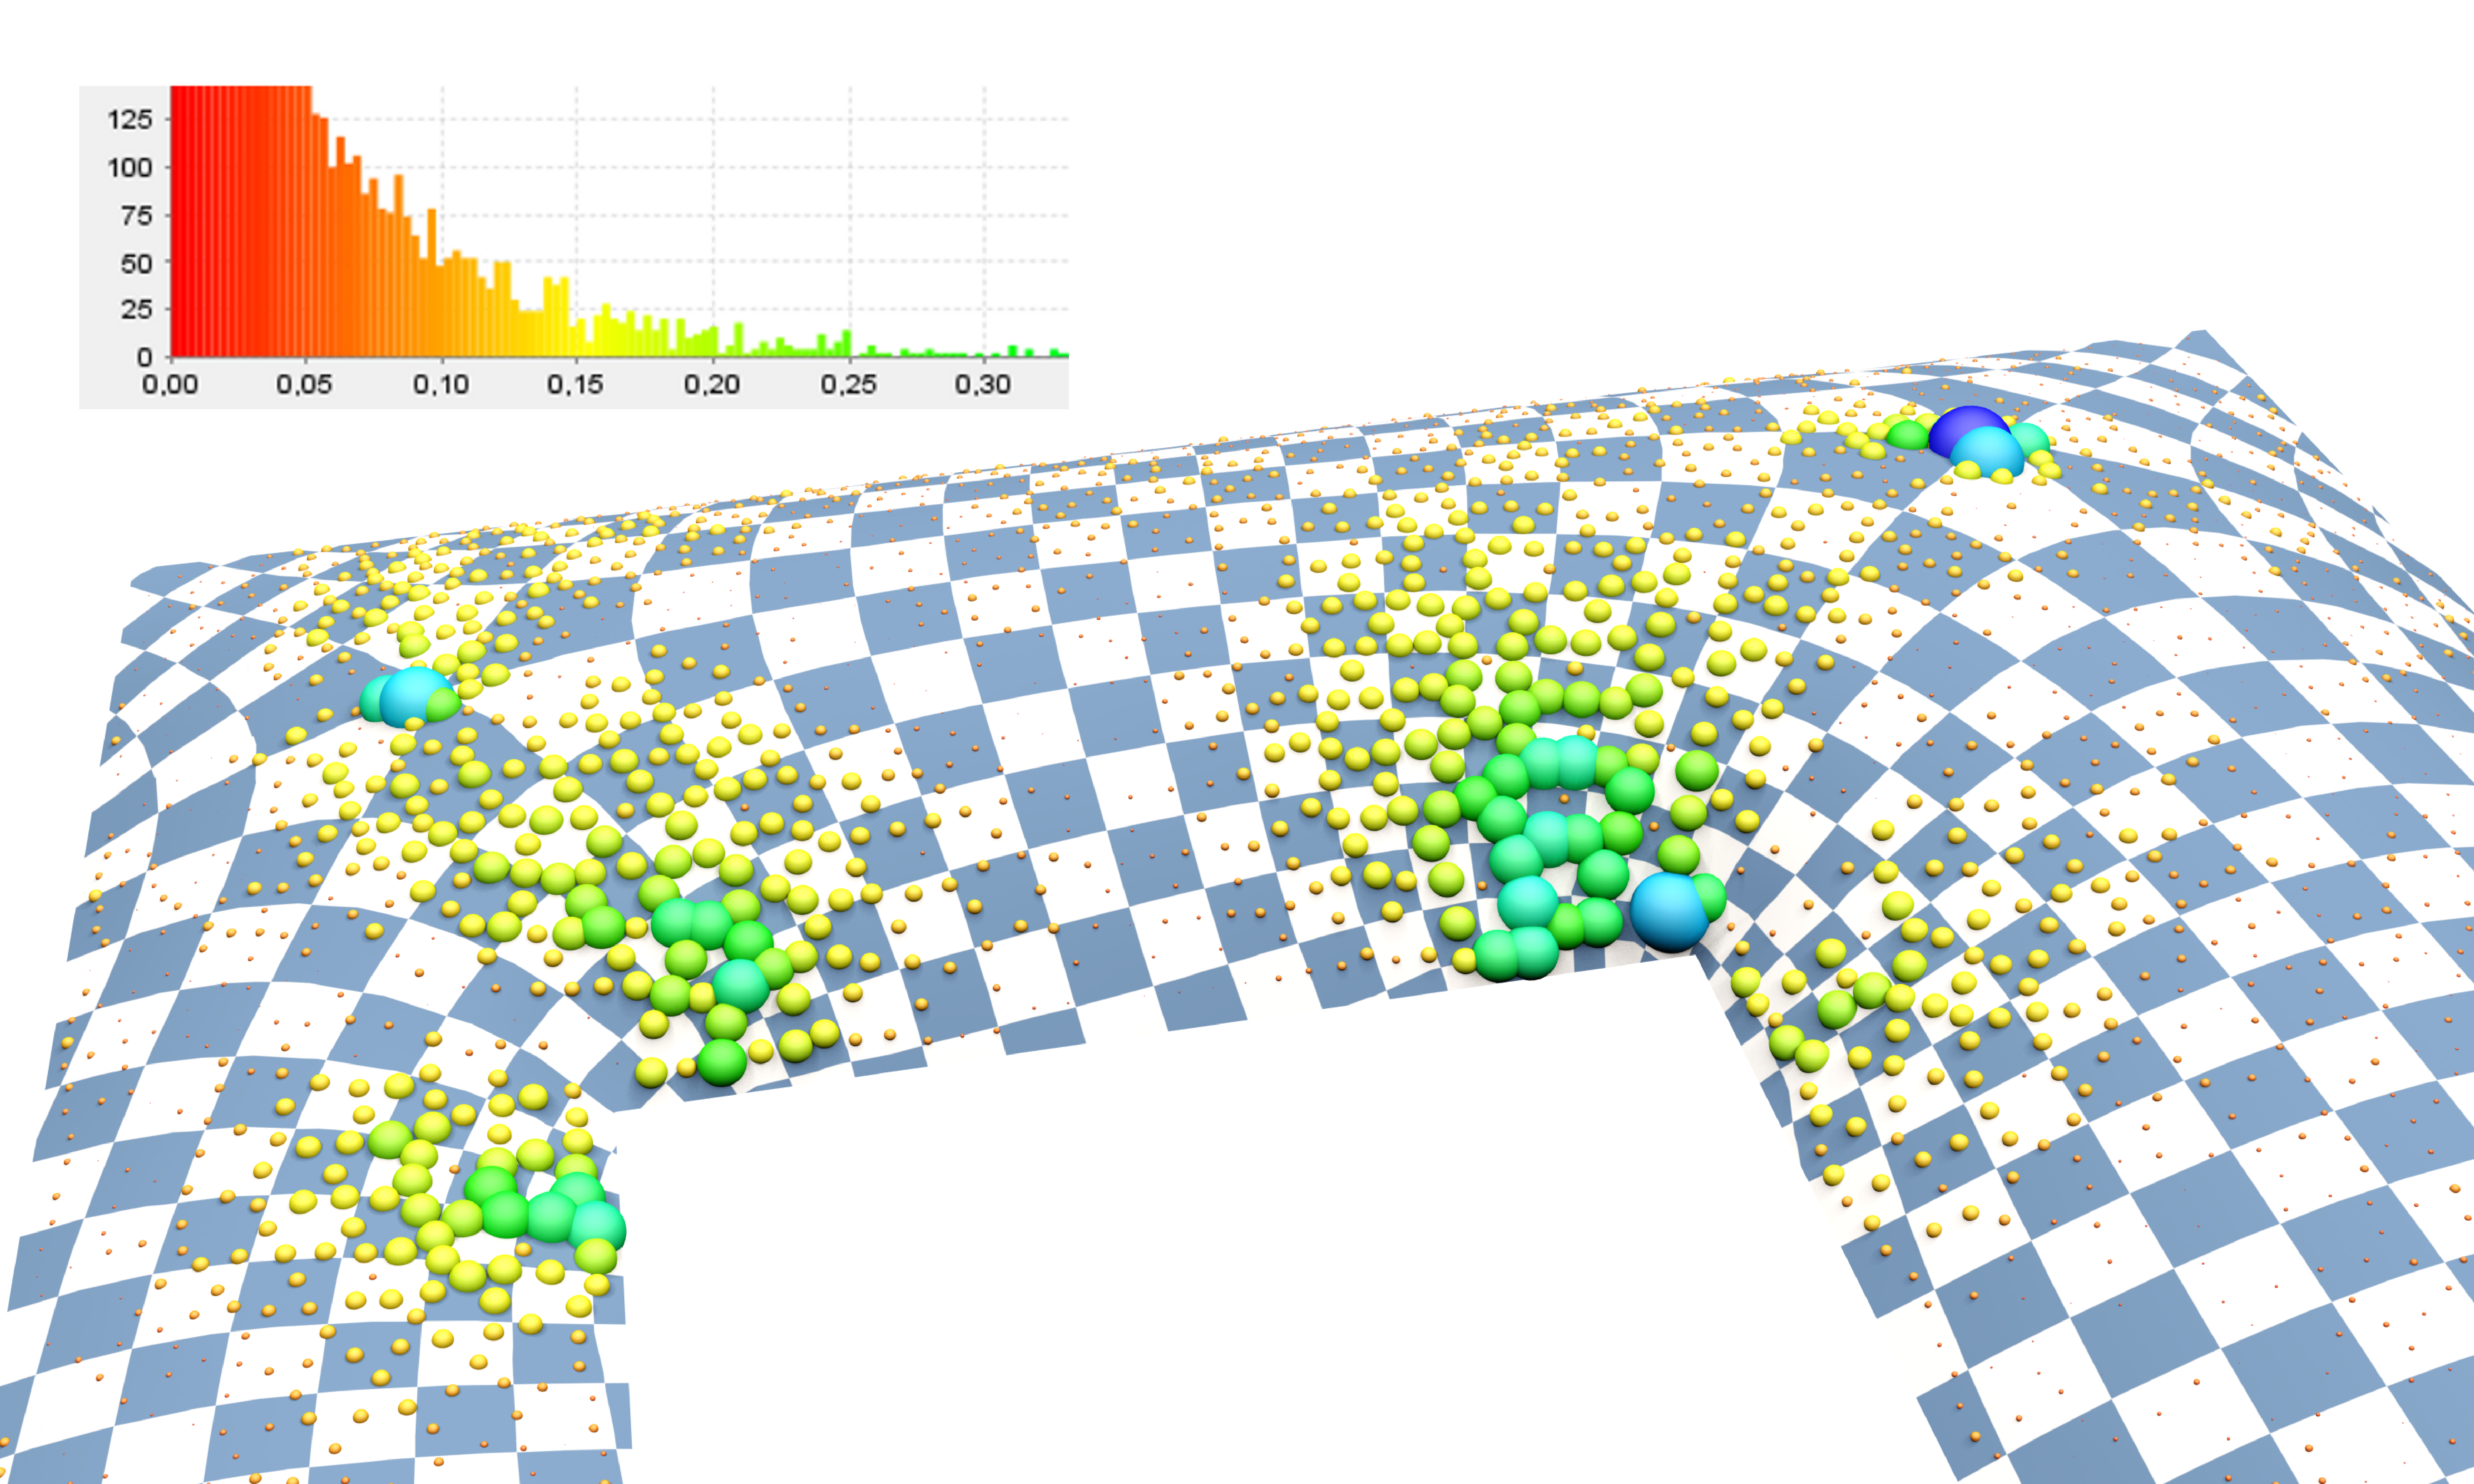
\includegraphics[width=\linewidth]{image/aag2012/dach01_quality_highres.pdf}
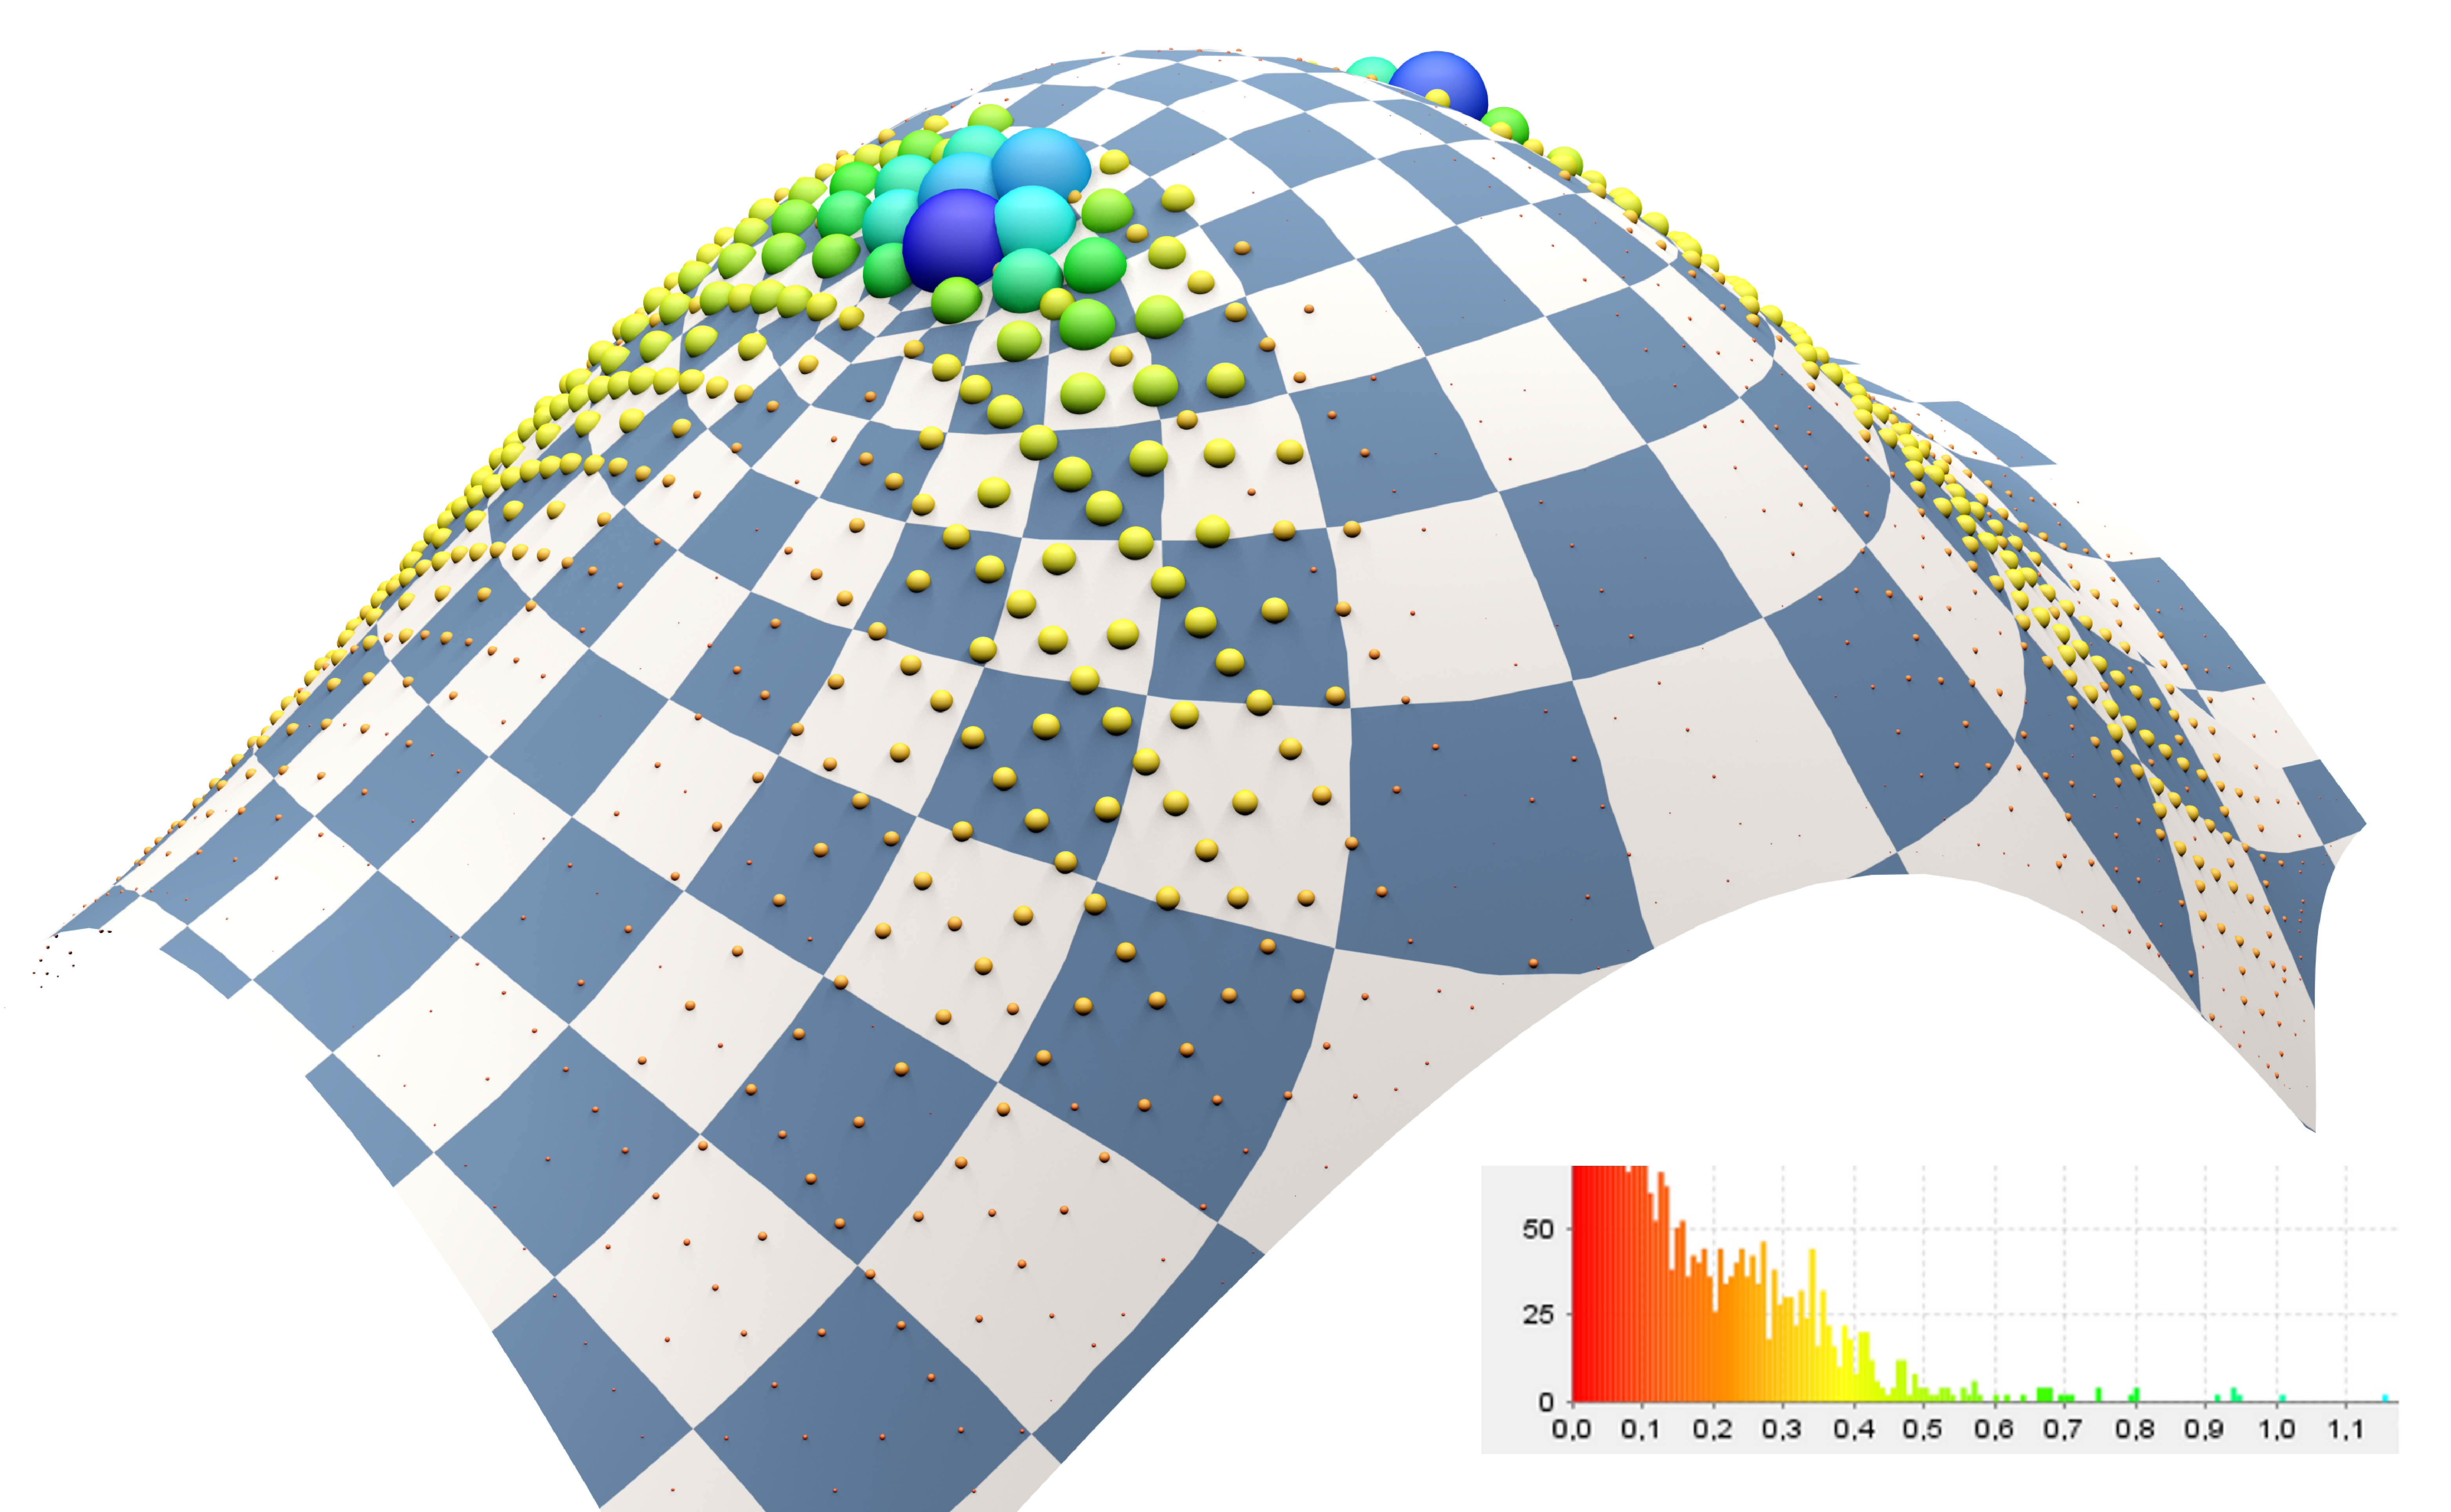
\includegraphics[width=\linewidth]{image/aag2012/dach02_quality_highres.pdf}
\caption[Parameterization quality plot]{The quality of the parameterization is measured in radians per
edge of the underlying triangulation. The checkerboard texture indicates the parameter
lines of the map. Small (red and yellow) beads represent good curvature direction quality, big
beads (green and blue) represent high deviation. The color of the histogram
corresponds to the color of the beads. Note that the mean error of the \textsc{Roof} 
surface (top) is half the error of the \textsc{Dome}. See also Table~\ref{tab:quality} 
for detailed quality measures of the other surfaces.}
\label{fig:quality}
\end{figure}
With the quasiisothermic modulus~$Q^\alpha$ on edges introduced in
Equation~(\ref{eq:quasiisothermicity}) we are now able to measure the 
quality of our parameterizations. 


There are two kinds of examples to consider: The first class of meshes stems from
smooth surfaces that admit conformal curvature line parameterizations, i.e.,
triangulations approximating isothermic surfaces. The second class consists of
arbitrary non-isothermic surfaces. For almost isothermic surfaces we expect
our parameterization to reconstruct the isothermic coordinates up to numerical
precision and hence $Q^\alpha$ to be reasonably small. For non-isothermic
surfaces we achieve the correct directions on the boundary but lack accuracy in
the interior. In Table~\ref{tab:quality} we summarize the numerical results
obtained from the surfaces of Figure~\ref{fig:all_mesh}.

\bigskip
\noindent \textbf{Isothermic surfaces.} The class of smooth isothermic
surfaces contains surfaces of constant mean curvature, surfaces of revolution,
and conic sections.  We use the \textsc{Minimal} example as an instance of an 
isothermic surface with mean curvature zero (Figure~\ref{fig:all_mesh}b). 
As expected this surface exhibits the highest curvature line quality of all tested 
meshes. The error however cannot vanish completely since the surface's curvature 
field contains singularities. In the vicinity of these points the numerical curvature 
directions contain significant amounts of noise.

\bigskip
\noindent \textbf{Non-isothermic surfaces.} Non-isothermic surfaces are
surfaces that do not admit a parameterization with conformal curvature lines. We
investigate
the properties of surfaces (a), (c), and (d) displayed in
Figure~\ref{fig:all_mesh}.

\begin{table}
\centering
\begin{tabular*}{0.7\linewidth}{l|l|l|l|l|l}
 & $\#E$ & $\#\partial E$ & $Q^\alpha_{\mathrm{mean}}$ & $Q^\alpha_{\mathrm{max}}$ &
$Q^\alpha_{\mathrm{\sigma}}$ \\ \hline
\textsc{Minimal} & 6260 & 450 & 0.036 & 0.603 & 0.033\\
\textsc{Teaser} & 17550 & 1000 & 0.057 & 1.20 & 0.066\\
\textsc{Roof} & 3766 & 470 & 0.051 & 0.610 & 0.059 \\
\textsc{Dome} & 1900 & 350 & 0.133 & 1.52 & 0.157
\end{tabular*}  
\caption{The curvature line approximation quality of the examples. $\#\partial
E$ are the number of boundary edges. $Q^\alpha_{\mathrm{\sigma}}$ is the standard
deviation of $Q^\alpha$.}
\label{tab:quality}
\end{table}

The \textsc{Teaser} surface was created as a minimizer of a spring functional
fixing the boundary and modelling interior edges as springs of rest length
zero. It is not far away from a minimal surface with the same boundary. The
curvature
line pattern however differs substantially as it contains singularities whereas
the minimal surface with this boundary curve does not. The quality of the
curvature line pattern is also very high. The mean angle error of the numerical
directions is $3.2$ degrees. Note that the deviation $Q_\sigma$ from the mean
value is also very low. For this surface the coordinates generated by our
algorithm are a globally good approximation to conformal curvature lines.

A quality plot of the \textsc{Roof} surface (Figures~\ref{fig:all_mesh}d and
\ref{fig:dach01_directions}) is shown in Figure~\ref{fig:quality}. Surprisingly, 
the quality of the curvature lines is as high as in the \textsc{Teaser} or the 
\textsc{Minimal} case. This suggests that a slight variation of the surface 
yields an isothermic surface. See also Figure~\ref{fig:dach01_directions} for 
a visual impression of the quality of the curvature lines.

The \textsc{Dome} model (Figure~\ref{fig:all_mesh}c) is created from a NURBS
surface. The quality plot (Figure~\ref{fig:quality}) reveals
areas of high angle deviation especially around the singularities. 
Other areas, in particular those near the boundary, are of high curvature line quality. 
The distance to the nearest isothermic surface is expected to be larger than in the
previous examples. More evidence for this is given in
Section~\ref{sec:s-isothermic}.

\bigskip
\noindent\textbf{Discussion.}
Our parameterization scheme works well for surfaces that are not too far away
from surfaces that possess isothermic coordinates. In the case of surfaces
stemming from minimal or constant mean curvature surfaces we get almost perfect
approximation quality of curvature lines. These are surfaces that are
particularly interesting when designing beam layouts for roof structures that
where form-found. For
other surfaces the parameterization is conformal and the parameter line pattern
captures the combinatorics of the curvature line pattern while approximating
the curvature line geometry.
There are of course surfaces for which our method is not applicable.
If the boundary is too short compared to the overall size of the surface we 
cannot expect the solution to follow curvature lines as the distance to the boundary 
increases.


\section{Discrete s-isothermic surfaces}
\label{sec:s-isothermic}

\begin{figure}
\centering
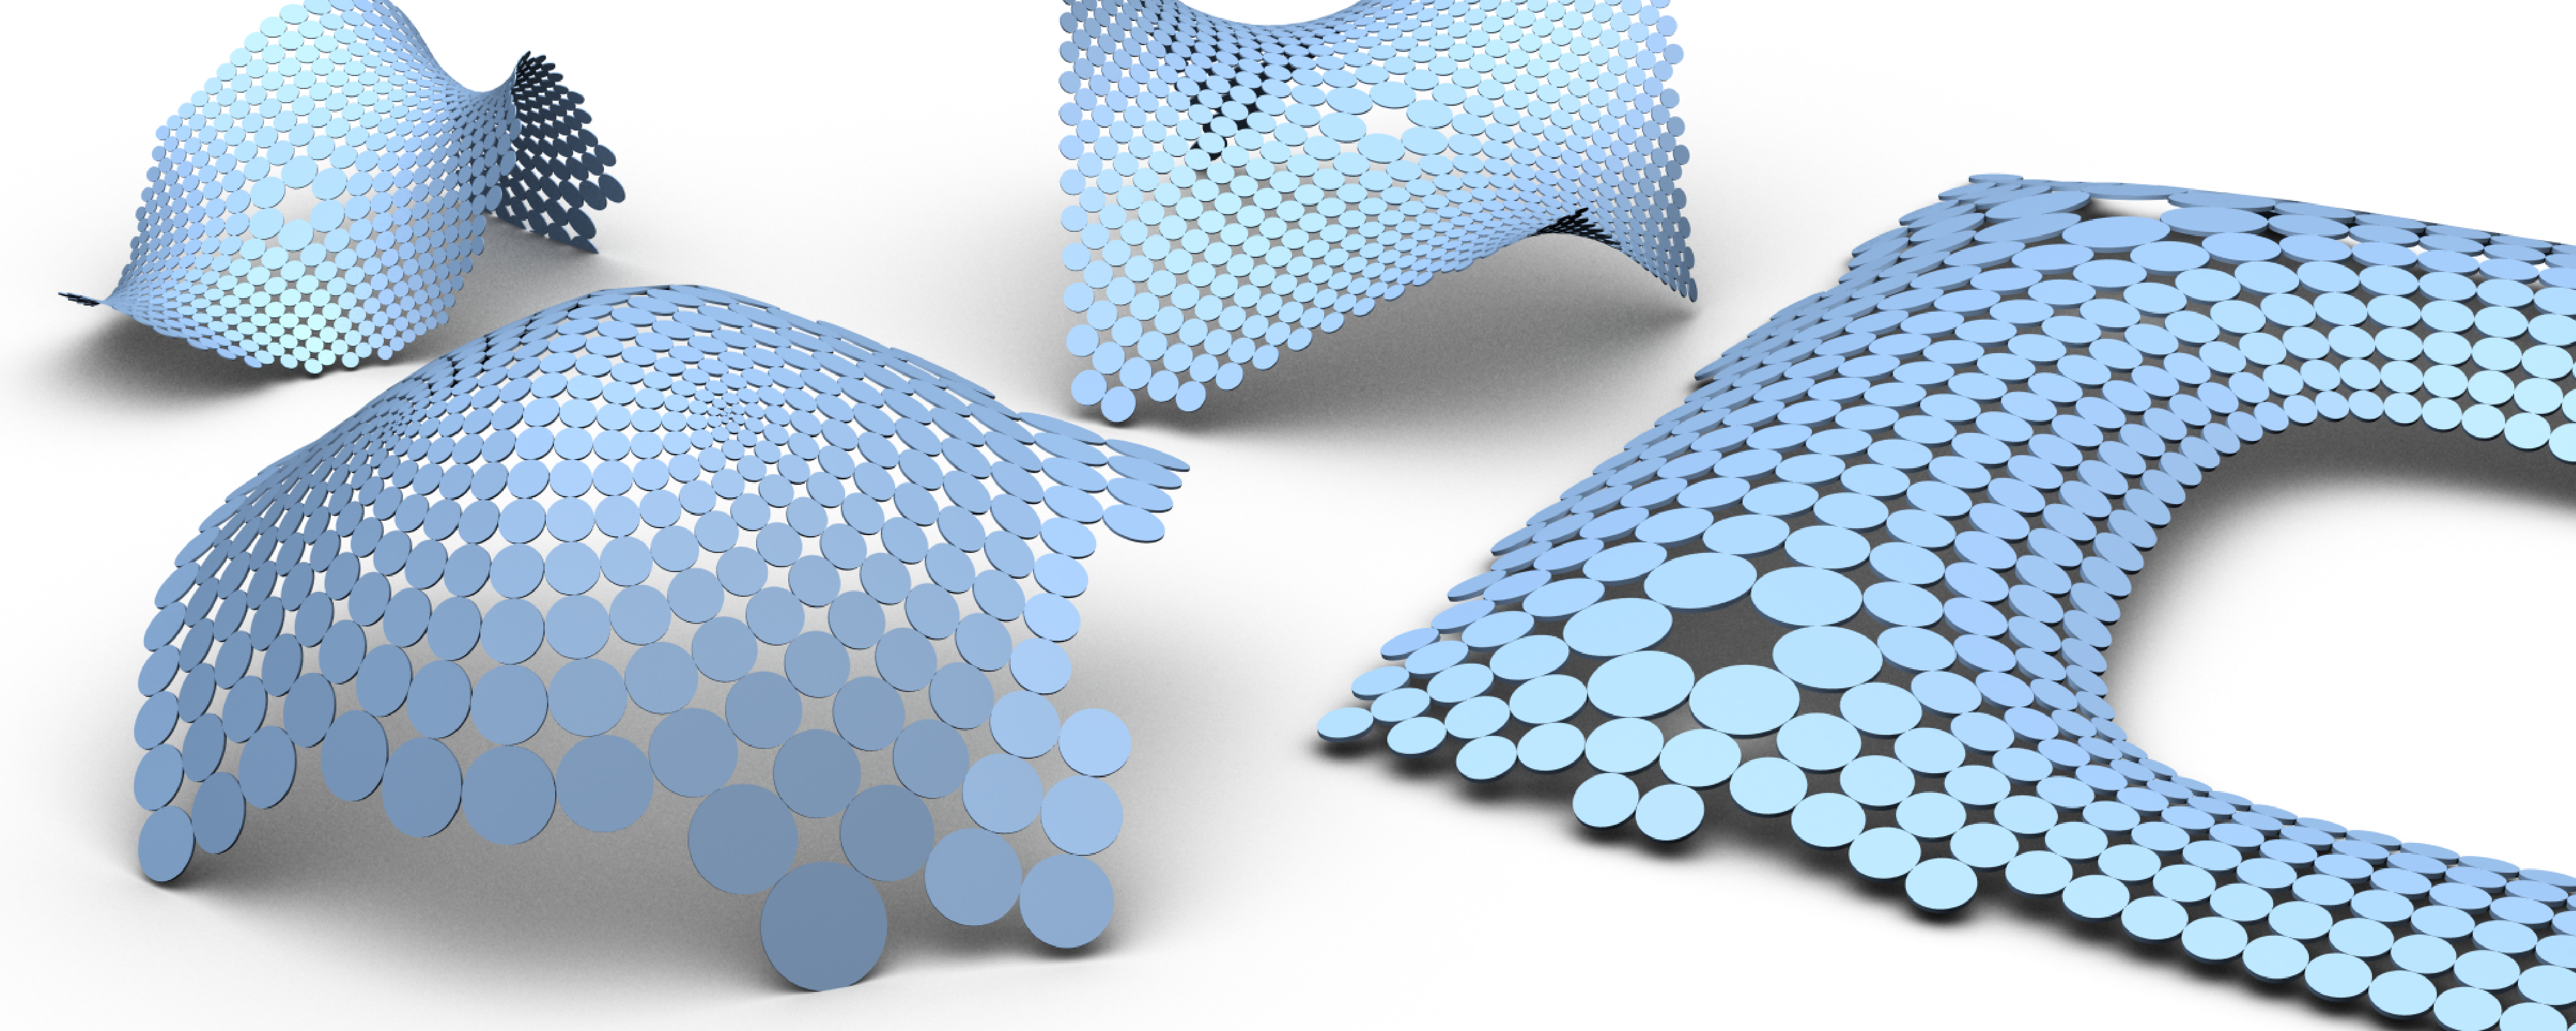
\includegraphics[width=\linewidth]{image/aag2012/all_circles.pdf}
\caption[S-isothermic meshes]{S-isothermic meshes created from the models presented in
Figure~\ref{fig:all_mesh}.
The inner quadrilaterals are optimized towards touching incircles. A series of
touching circles in a row can be interpreted as discrete curvature line.}
\label{fig:s_isothermic}
\end{figure}

Starting with a quasiisothermically parameterized mesh with low modulus 
we now aim to create discrete s-isothermic surfaces that
stay in the vicinity of the input surface. S-isothermic surfaces were
introduced by Bobenko and Pinkall~\cite{BobenkoP1996}: A quadrilateral mesh
is \mbox{\emph{s-isothermic}} if (i) all the quadrilaterals are planar, (ii)
all faces have incircles, and (iii) the incircles of adjacent quadrilaterals
touch.
Figure~\ref{fig:s_isothermic} displays s-isothermic surfaces derived from our
parametrizations shown in Figure~\ref{fig:all_mesh}.

\subsubsection{Variational Principle}

\begin{figure}
\centering
\resizebox{0.4\textwidth}{!}{\input{figures/e_touching_circles.pdf_t}}
\caption{Labels for the touching-circle
functional at an edge. The circles touch 
if the ratio $\cot\left(\beta^i/2\right)/\cot\left(\beta^j/2\right)$ is equal on both sides of the edge.}
\label{fig:functional}
\end{figure}

In this section we introduce an energy whose minimizers are s-isothermic
surfaces. We denote quadilaterals by $ijkm\in F$ where the indices are in 
cyclic order.
The s-isothermic energy $E_S$ consists of three parts:
\begin{equation}
  E_S := 
  \lambda_1 E_{\mathrm{planar}} + 
  \lambda_2 E_{\mathrm{incircle}} + 
  \lambda_3 E_{\mathrm{touch}}
\end{equation}
The planarity energy $E_{\mathrm{planar}}$ penalizes non-planar quadrilateral
faces. For each quad it can be defined either by the distance of the diagonals
(an idea attributed to Peter Schr\"oder~\cite{PottmannSBSWBW2008}) or the
volume of the tetrahedron spanned by the
four vertices. We give the formula for the former here. 
\begin{equation}
E_{\mathrm{planar}} = \sum_{\mathrm{\it{ijkm}} \in F} \frac{\left<\Delta_{\mathrm{\it{ji}}},\Delta_{\mathrm{\it{mj}}} \times \Delta_{\mathrm{\it{ki}}}\right>^2}
{\Vert\Delta_{\mathrm{\it{mj}}} \times \Delta_{\mathrm{\it{ki}}}\Vert^2}
\end{equation}
Here $\Delta_{ij}$ is the vector pointing from vertex $i$ to $j$.

For $E_{\mathrm{incircle}}$ we use the energy defined by Schiftner~\emph{et~al.}~\cite{SchiftnerHWP2009} based on the fact that the sum of opposite edge
lengths must be equal for a planar quad to possess an incircle.
\begin{equation}
E_{\mathrm{incircle}} = \sum_{\mathrm{\it{ijkm}} \in F} \left( l_{\mathrm{\it{ij}}} + 
l_{\mathrm{\it{km}}} - l_{\mathrm{\it{jk}}} - l_{\mathrm{\it{mi}}} \right)^2
\end{equation}
The energy
$E_{\mathrm{touch}}$ is a new energy that enforces touching incircles
if faces are planar and possess incircles.  It is defined per edge, see
Figure~\ref{fig:functional} for the exact labeling of the angles at one edge.
For an interior edge $ij\in E$ we define
\begin{equation}
  E_{\mathrm{touch}}(\mathrm{\it{ij}})=
  \left(\cot\frac{\beta^j_l}{2}\cot\frac{\beta^i_r}{2} - 
\cot\frac{\beta^j_r}{2}\cot\frac{\beta^i_l}{2}\right)^2.
\end{equation}
On boundary edges the energy is zero. All energies can be formulated 
in terms of the vertex coordinates and the derivatives can be calculated explicitly.

Since all energies are in general non-convex we need a good initial guess to 
find meaningful minimizers of $E_S$.
S-isothermic minimal surfaces converge to isothermic parameterizations of
smooth minimal surfaces~\cite{BobHofSpr06}. For general s-isothermic surfaces
this is an open conjecture. The parameterizations obtained in
Section~\ref{sec:parametrization} are good candidates to start from with the
optimization of the functional.
%numerics
We use the non-linear optimization package PETSc/TAO~\cite{petsc-web-page,
tao-user-ref} and its java binding~\cite{jpetsctao-web-page} to find
minimizers of $E_S$. Figure~\ref{fig:convergence} shows convergence plots of
$E_S$ for the four models that were discussed in the previous section.
\begin{figure}
\centering
\resizebox{\textwidth}{!}{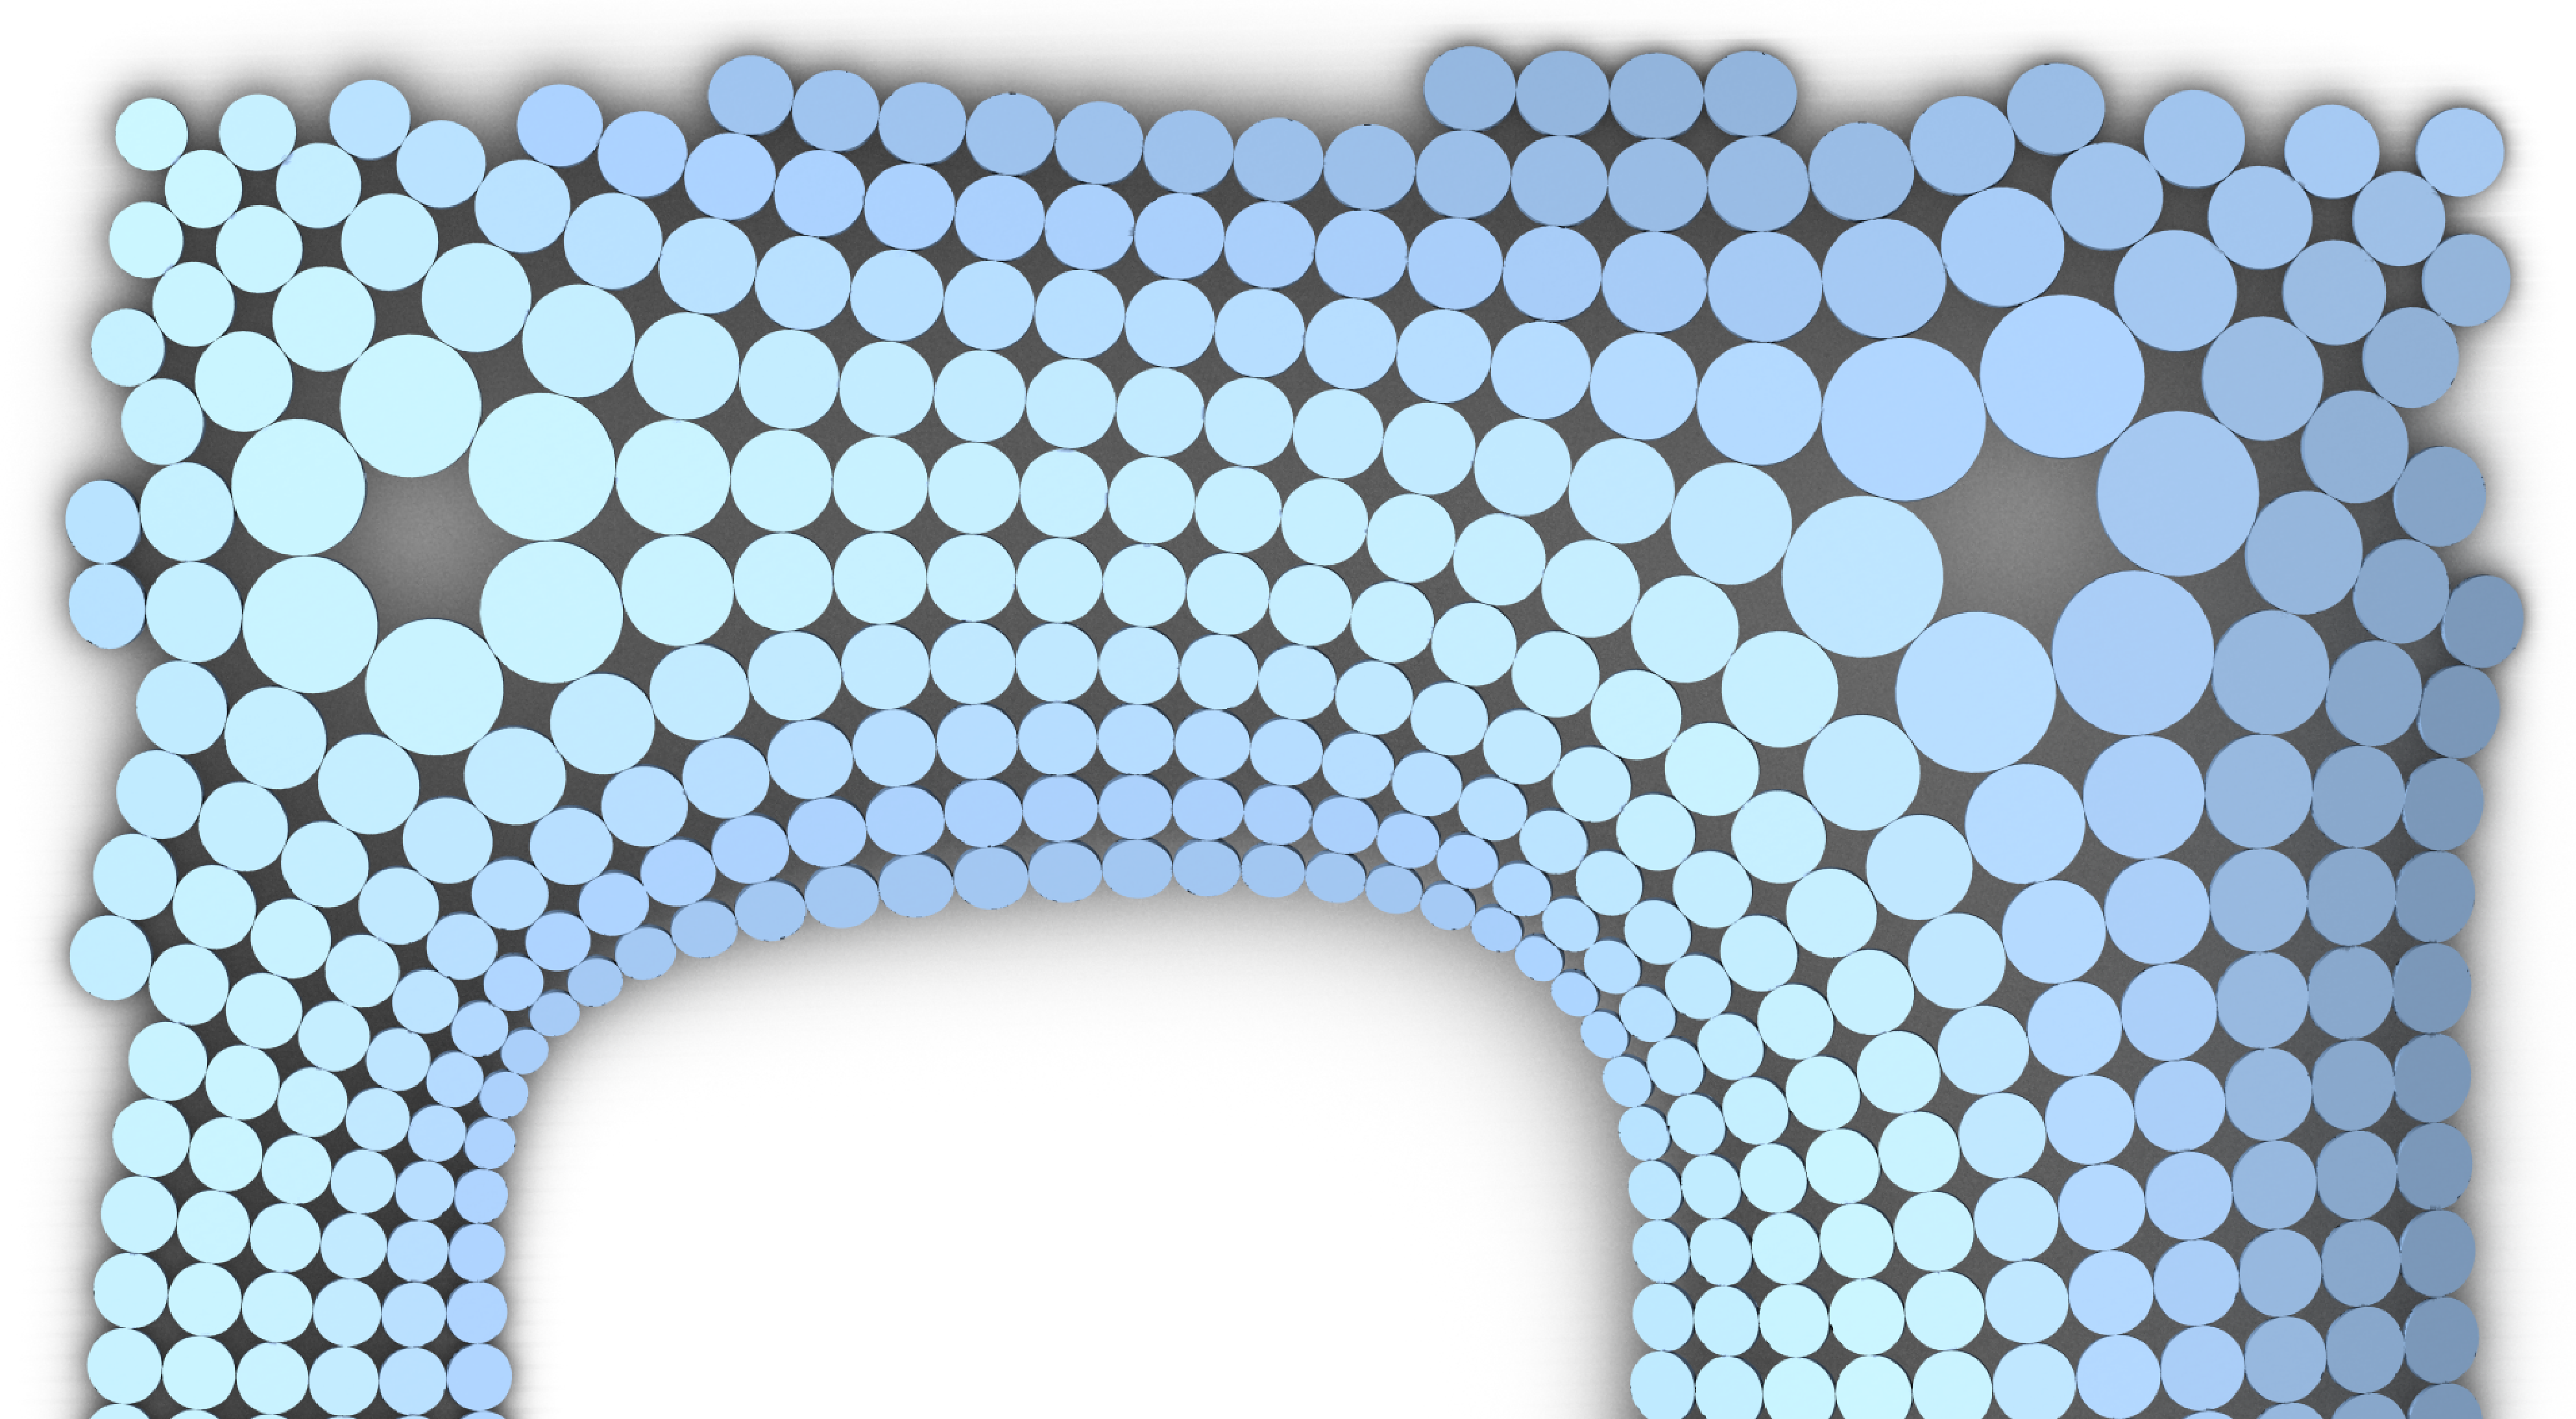
\includegraphics[width=\textwidth]{image/aag2012/dach_example01_circles.pdf}}
\caption{The s-isothermic circle packing on the \textsc{Roof} model in detail.}
\end{figure}

As seen in the quality analysis of Section~\ref{subsub:examples_quality}, the
\textsc{Teaser}, the \textsc{Minimal}, and the \textsc{Roof} models are
quasiisothermic surfaces with low modulus. For these models the corresponding s-isothermic
surface is also close to the input surface. Figure~\ref{fig:convergence} shows
the energy during the optimization. Here the three close-to-isothermic meshes
start with a lower energy than the \textsc{Dome} model. After the \textsc{Dome}
has passed some iterations it exhibits convergence properties similar to the
other models. As this surface converges against a discrete s-isothermic surface,
we observe a considerable change in shape during the first iterations
especially around the singularities.

\begin{figure}
\centering
\resizebox{0.7\textwidth}{!}{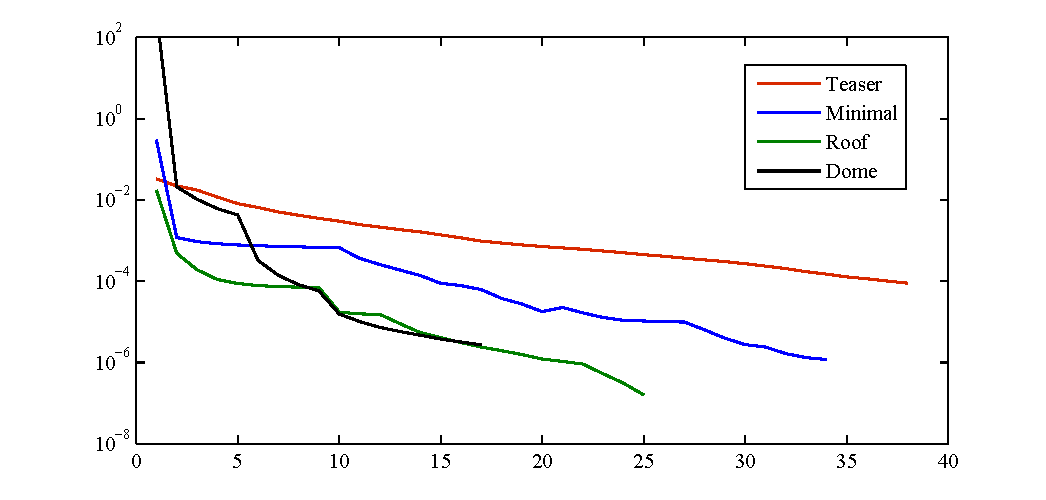
\includegraphics{image/aag2012/convergence_plots_embedded.pdf}}
\caption[Convergence behavior of $E_S$]{Convergence behavior of $E_S$ during optimization. We use the meshes 
displayed in Figure~\ref{fig:all_mesh} as initial guesses for the minimization. The
convergence of the Teaser geometry is slower due to the high complexity.}
\label{fig:convergence}
\end{figure}

\subsubsection{Isometric Deformations of Minimal Surfaces}
\label{sub:isometric}
\begin{figure*}
\centering
\resizebox{\textwidth}{!}{\input{figures/isometric.pdf_t}}
\caption{Non-trivial isometric deformations of a minimal surface. The edges of the dual
surface are rotated to create a \mbox{$1$-parameter} family of isometrically
deformed surfaces with 
period $2\pi$. The histogram shows the edge length error of the $90^\circ$ model
when compared 
with the initial surface. The mean edge length deviation of this model is $1.28\%$.}
\label{fig:isometric} 
\end{figure*}

Every smooth minimal surface possesses a $1$-parameter (associated) family of
non-trivial isometric deformations. All surfaces in this family have the same
Gau{\ss} map. For discrete s-isothermic minimal surfaces this construction is
discretized by Bobenko~\emph{et~al.}~\cite{BobHofSpr06}: Edge lengths and the conformality of the
parameterization are preserved. We need to introduce the concept of dual surface
to construct the family of isometric surfaces.

\noindent\textbf{The Dual Surface.}
In differential geometry for isothermic surfaces there is a notion of a dual
surface.  This dual or Christoffel transform is also an isothermic surface. Both
surfaces are parameterized with isothermic coordinates. This setup can be
discretized using the definition of discrete s-isothermic surfaces. The dual
surface can be constructed using the incircle structure of s-isothermic meshes.
We introduce consistent signs on edges on a discrete s-isothermic surface such
that opposite sides of the quads have the same sign and consecutive edges in a
quad have different signs. The dual mesh of a mesh $M$ will have parallel edges
calculated as follows: Let $e_{ij}=v_j-v_i$ be an edge vector of~$M$. Then the
dual edge vector $e_{ij}^*$ satisfies the following equation:
\[e_{ij}^* = \pm \frac{1}{r_i \cdot r_j} e_{ij}\]
where $r_i$ and $r_j$ are the distances from the vertex $v_i$ and $v_j$ to the
touching point of the incircles of incident faces at the edge~$e_{ij}$. For a
given
discrete s-isothermic mesh we can easily calculate the dual mesh by enumerating
the vertices along a spanning tree of edges. In Figure~\ref{fig:isometric} the
dual surface of the \textsc{Minimal} model is shown in the upper left hand
corner.  Via the dual surface we can now construct isometric deformations of
minimal surfaces.

\noindent\textbf{Deformation.}
The dual of a smooth minimal surface coincides with its Gau{\ss} map which is a
part of a sphere. This sphere may be multiply covered. For discrete s-isothermic
minimal surfaces this Gau{\ss} map is a part of a Koebe polyhedron, i.e., a
polyhedral surfaces with edges tangent to a sphere. On the Koebe polyhedron
every edge is rotated by a fixed angle in the tangent space of the sphere at the
points of tangency of the edge. The resulting edge vectors again form closed
quads and can be dualized. This dual surface has the same edge lengths as the
initial minimal surface.

For minimal quad meshes with touching incircles that were created using our
parameterization and the optimization step, the dual surface will be close to a
Koebe polyhedron. We use a least-squares-sphere to define a consistent tangent
space at the touching points of incircles with the edges. The resulting
deformation of a given minimal surface is then close to isometric. To distribute
the isometry error on the edges we average over different roots of the layout
spanning tree. Surfaces that do not possess exact isometric deformations are
deformed approximative.

We apply this procedure to the \textsc{Minimal} model
\mbox{(Figure~\ref{fig:all_mesh}a)}. Figure~\ref{fig:isometric} shows the
surface together
with its dual and isometrically deformed versions with different turning angles.

\section{A discrete s-isothermic ellipsoid and its dual surface}
\label{sec:discrete_ellipsoid}

\begin{figure*}
\centering
\resizebox{\textwidth}{!}{
$\vcenter{\hbox{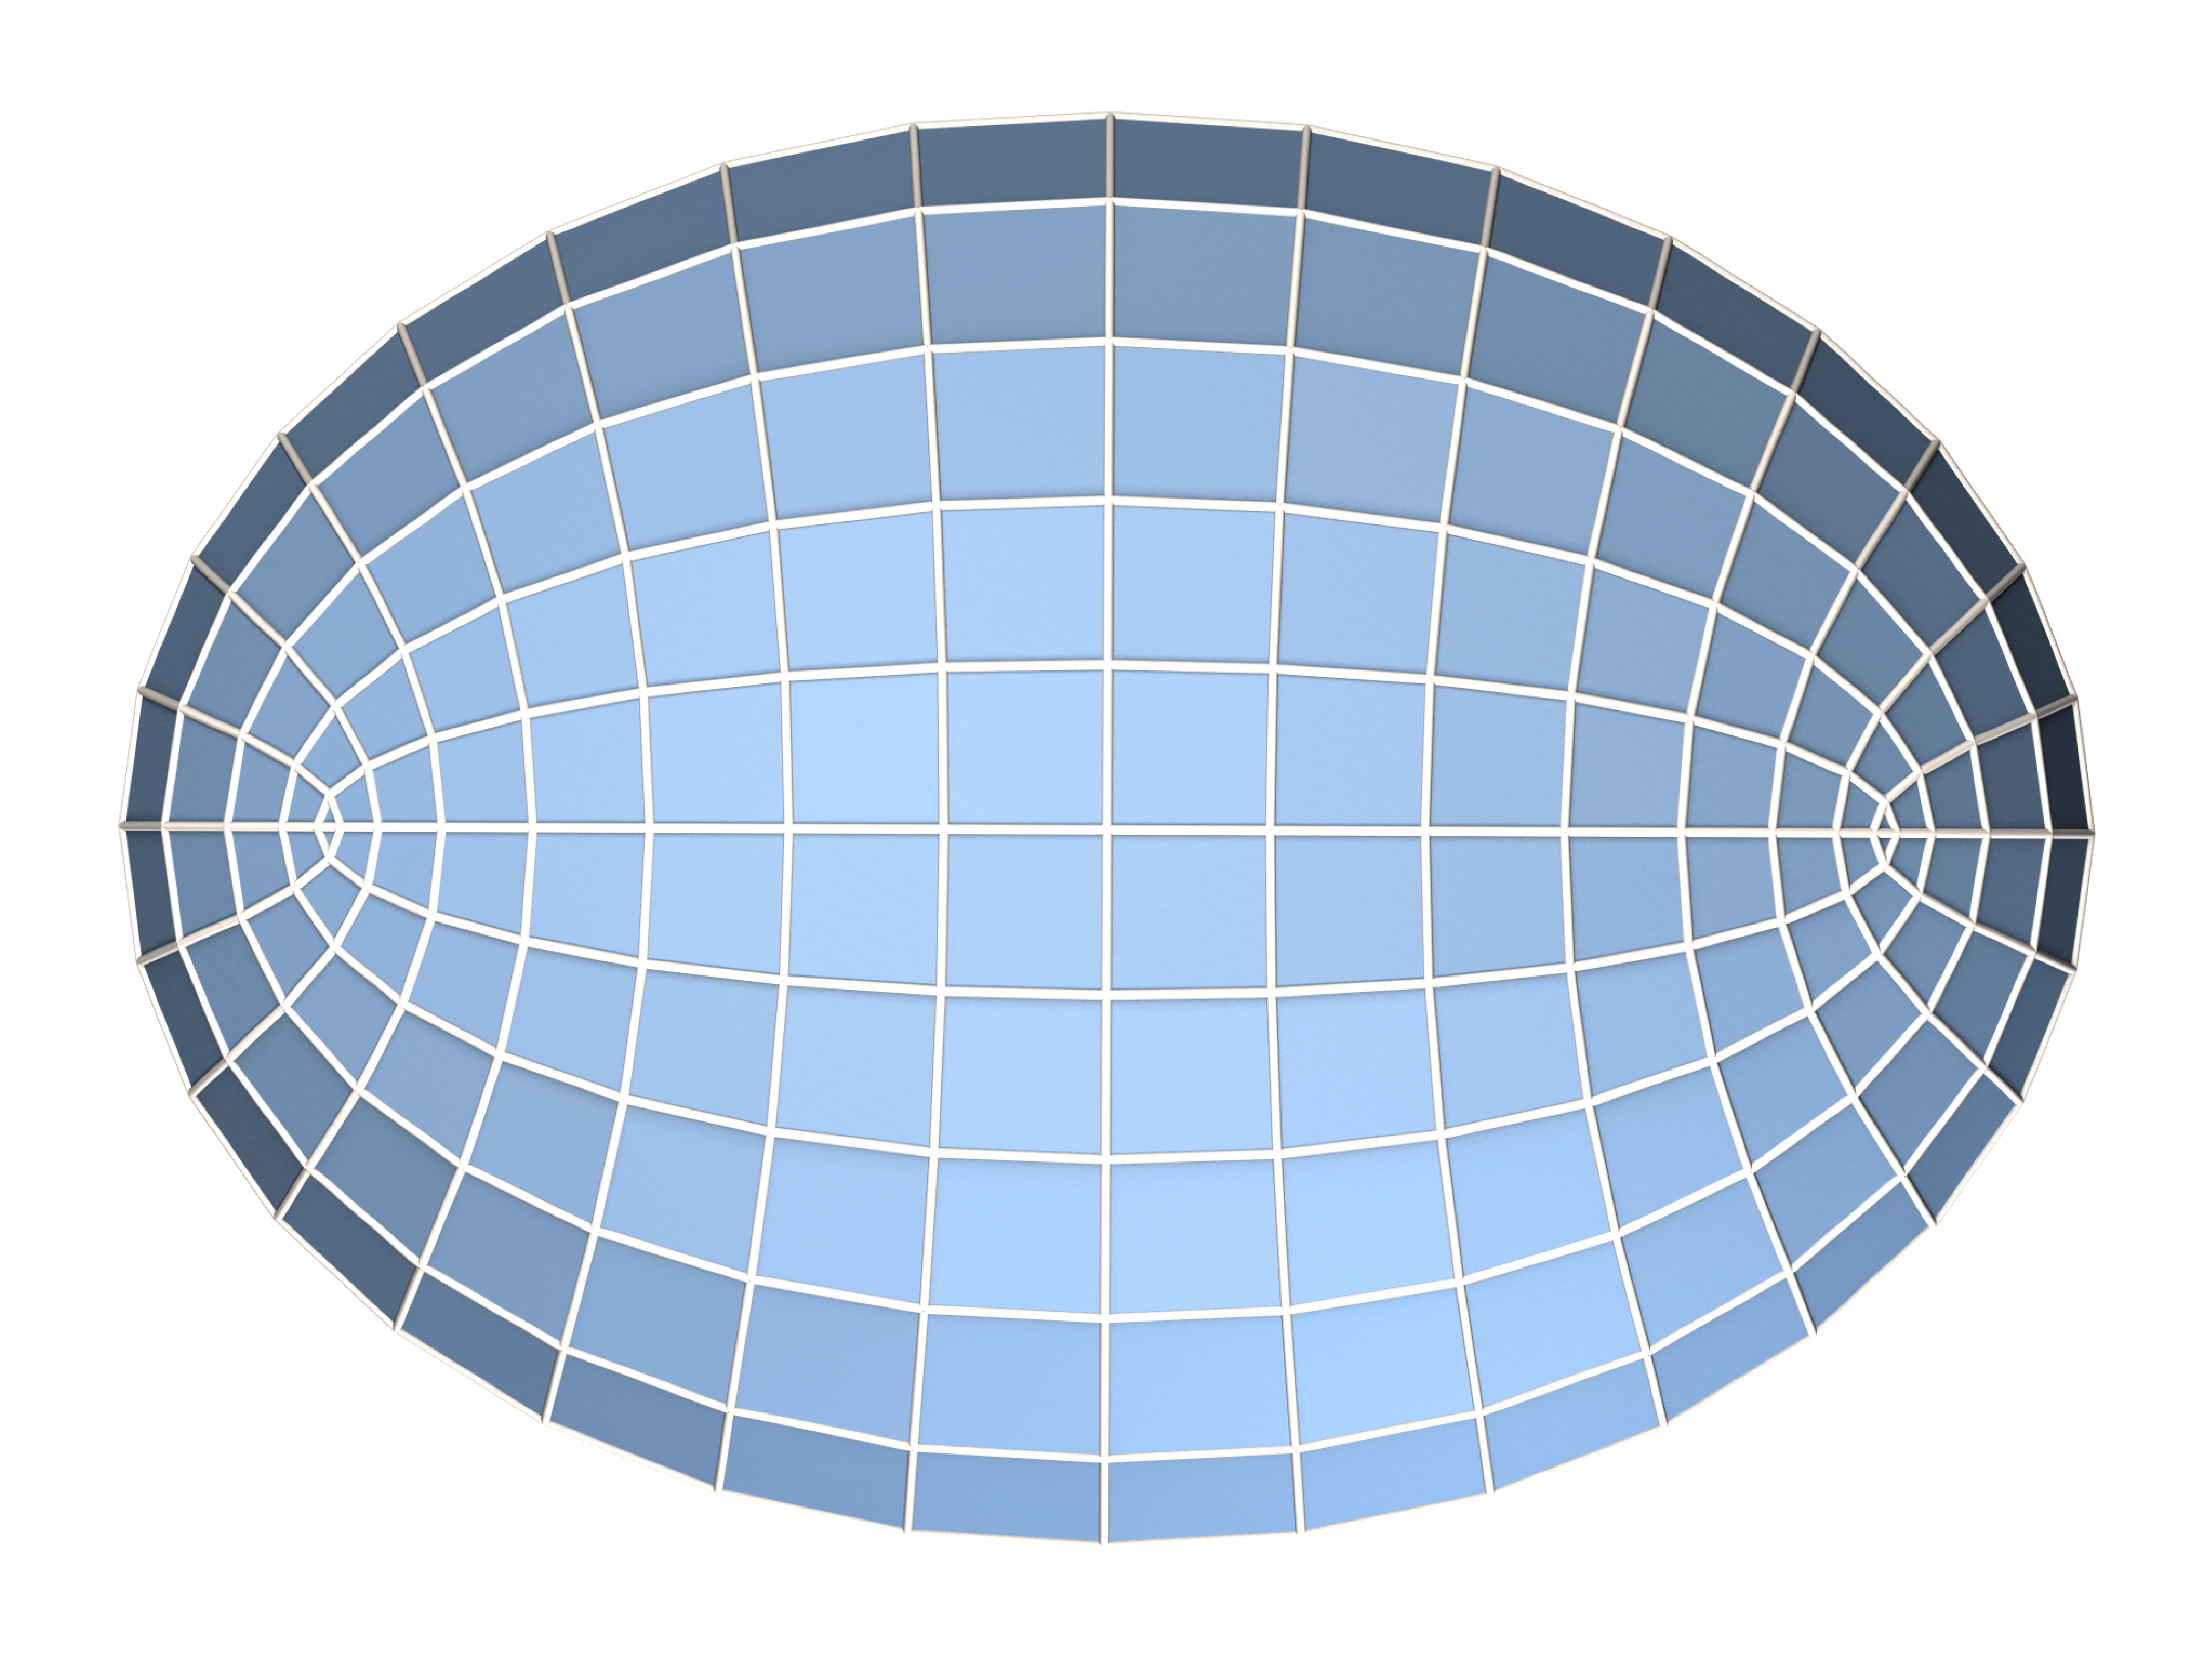
\includegraphics[width=0.5\textwidth]{image/ellipsoid01_top.pdf}}}$
$\vcenter{\hbox{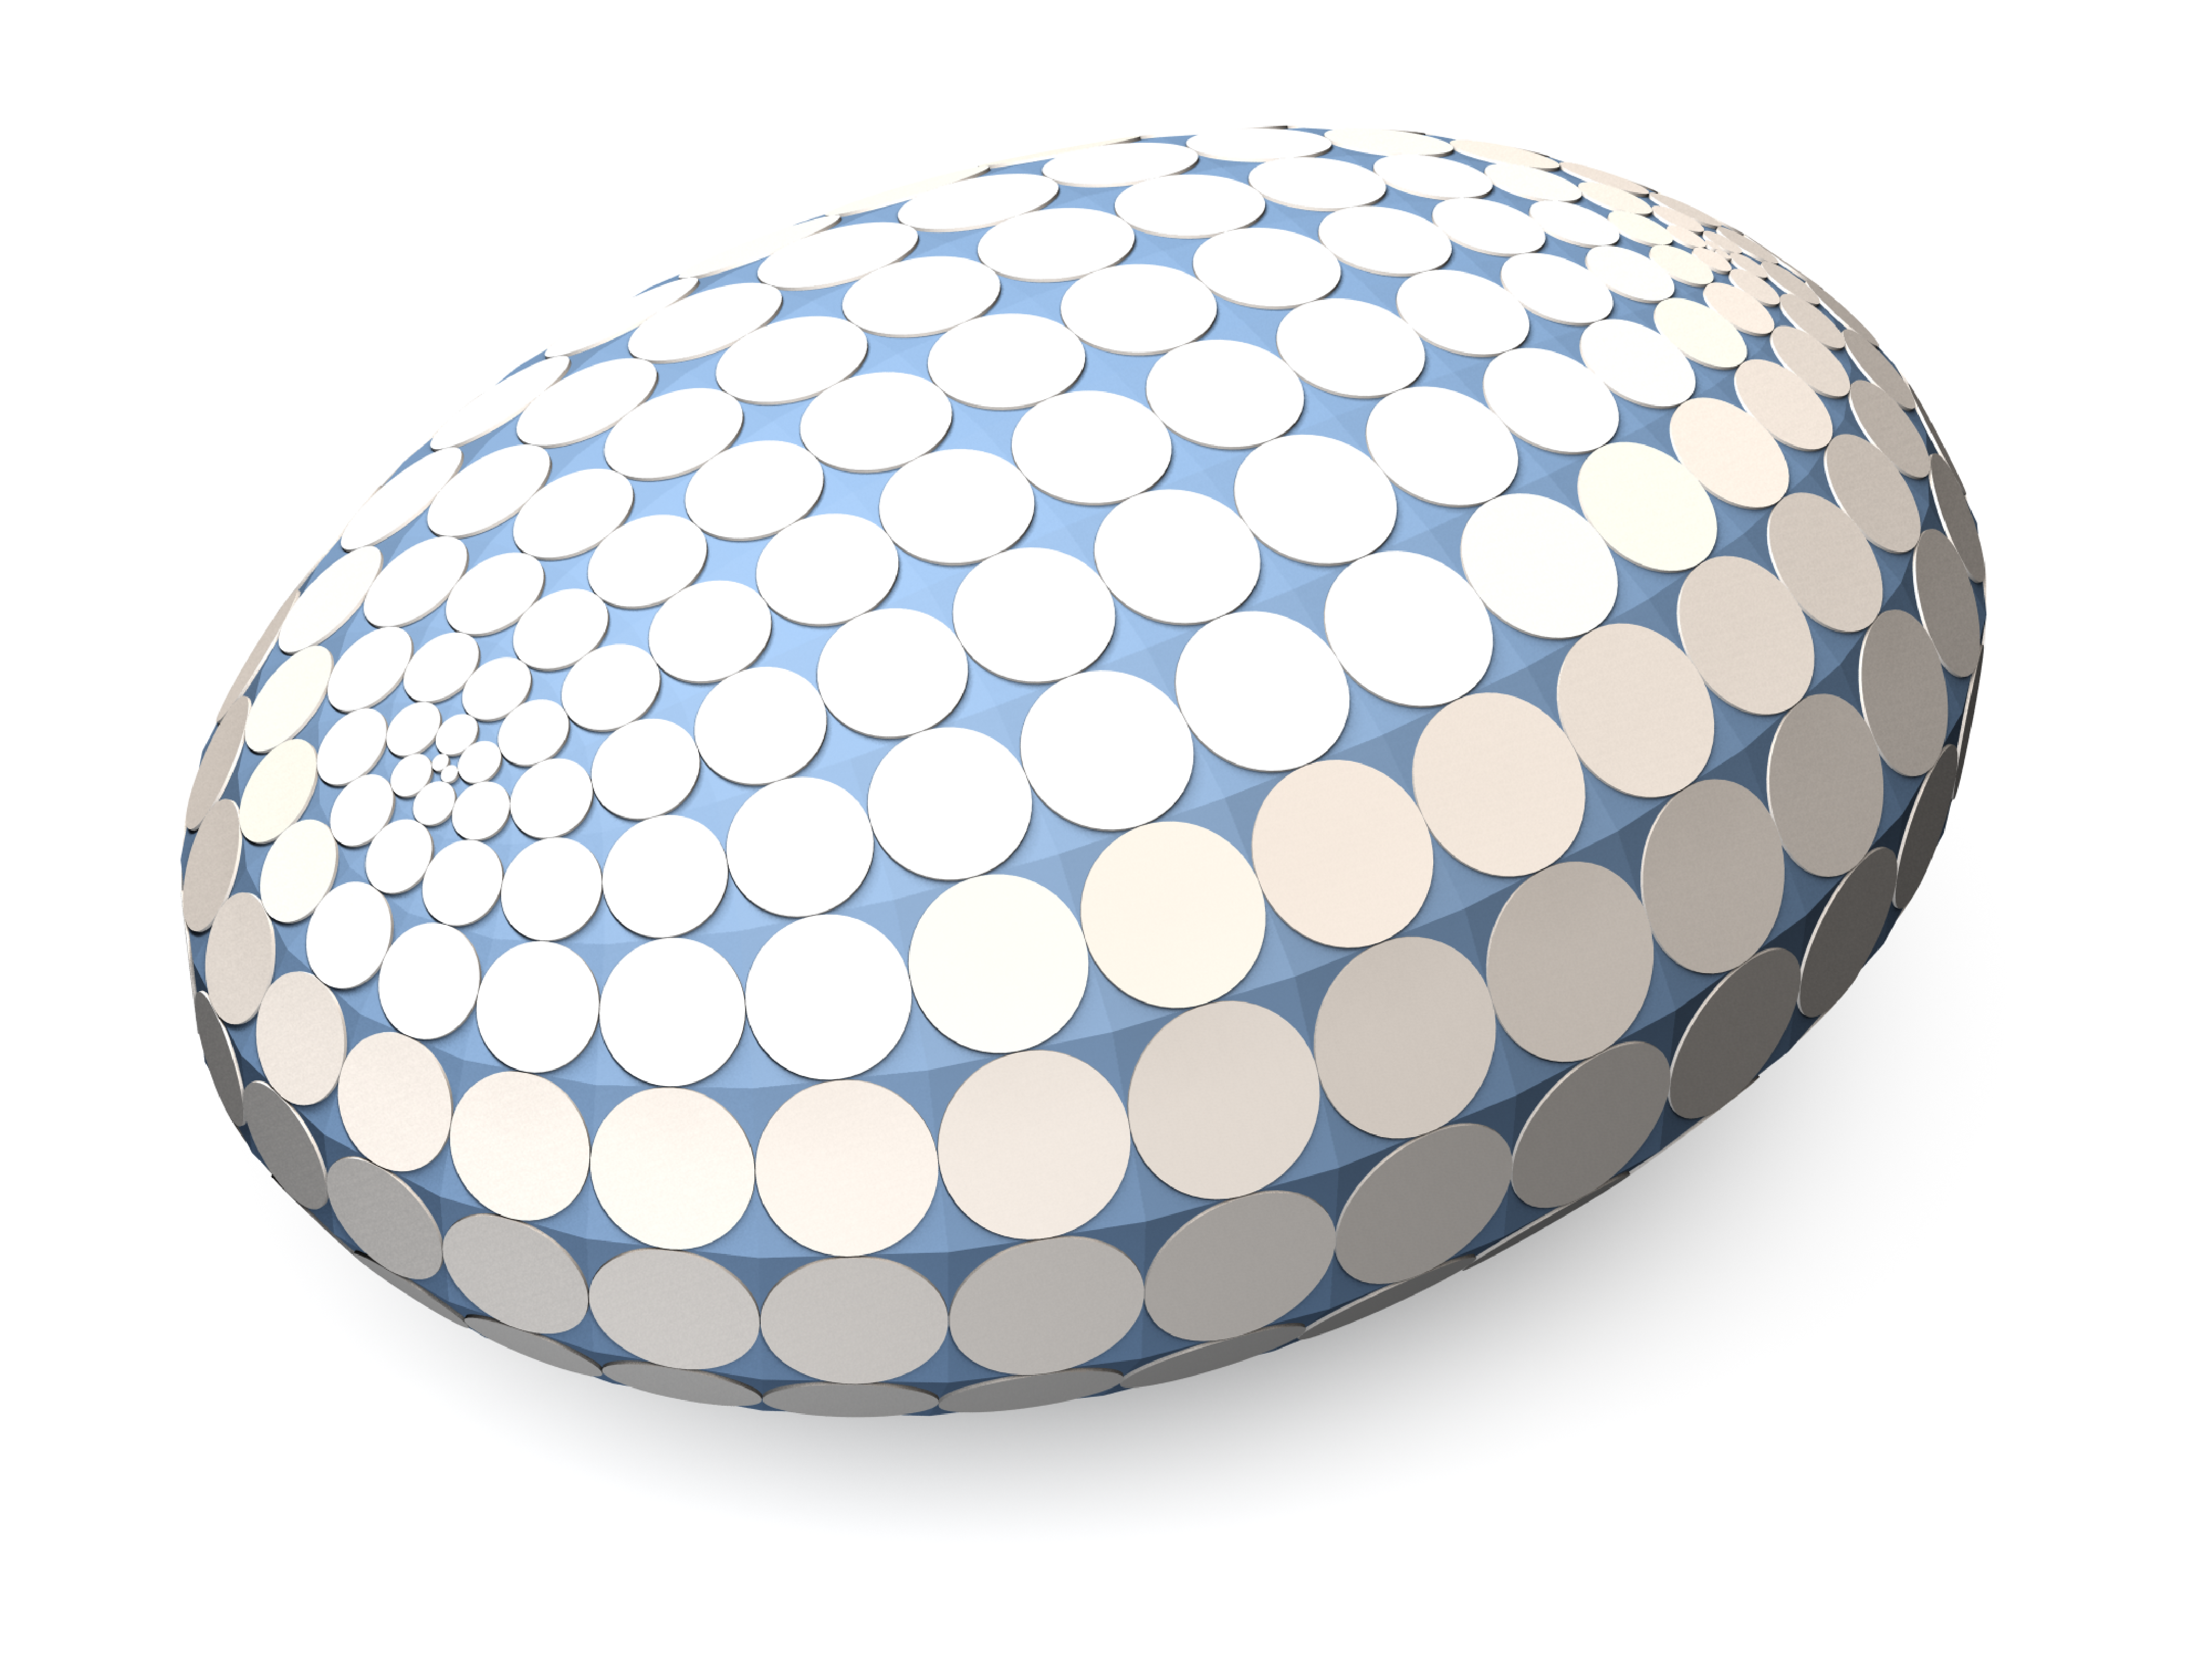
\includegraphics[width=0.5\textwidth]{image/ellipsoid01_disks.pdf}}}$
}
\caption{Discrete s-isothermic ellipsoid}
\label{fig:ellipsoid} 
\end{figure*}

\begin{figure}
\centering
\resizebox{\textwidth}{!}{
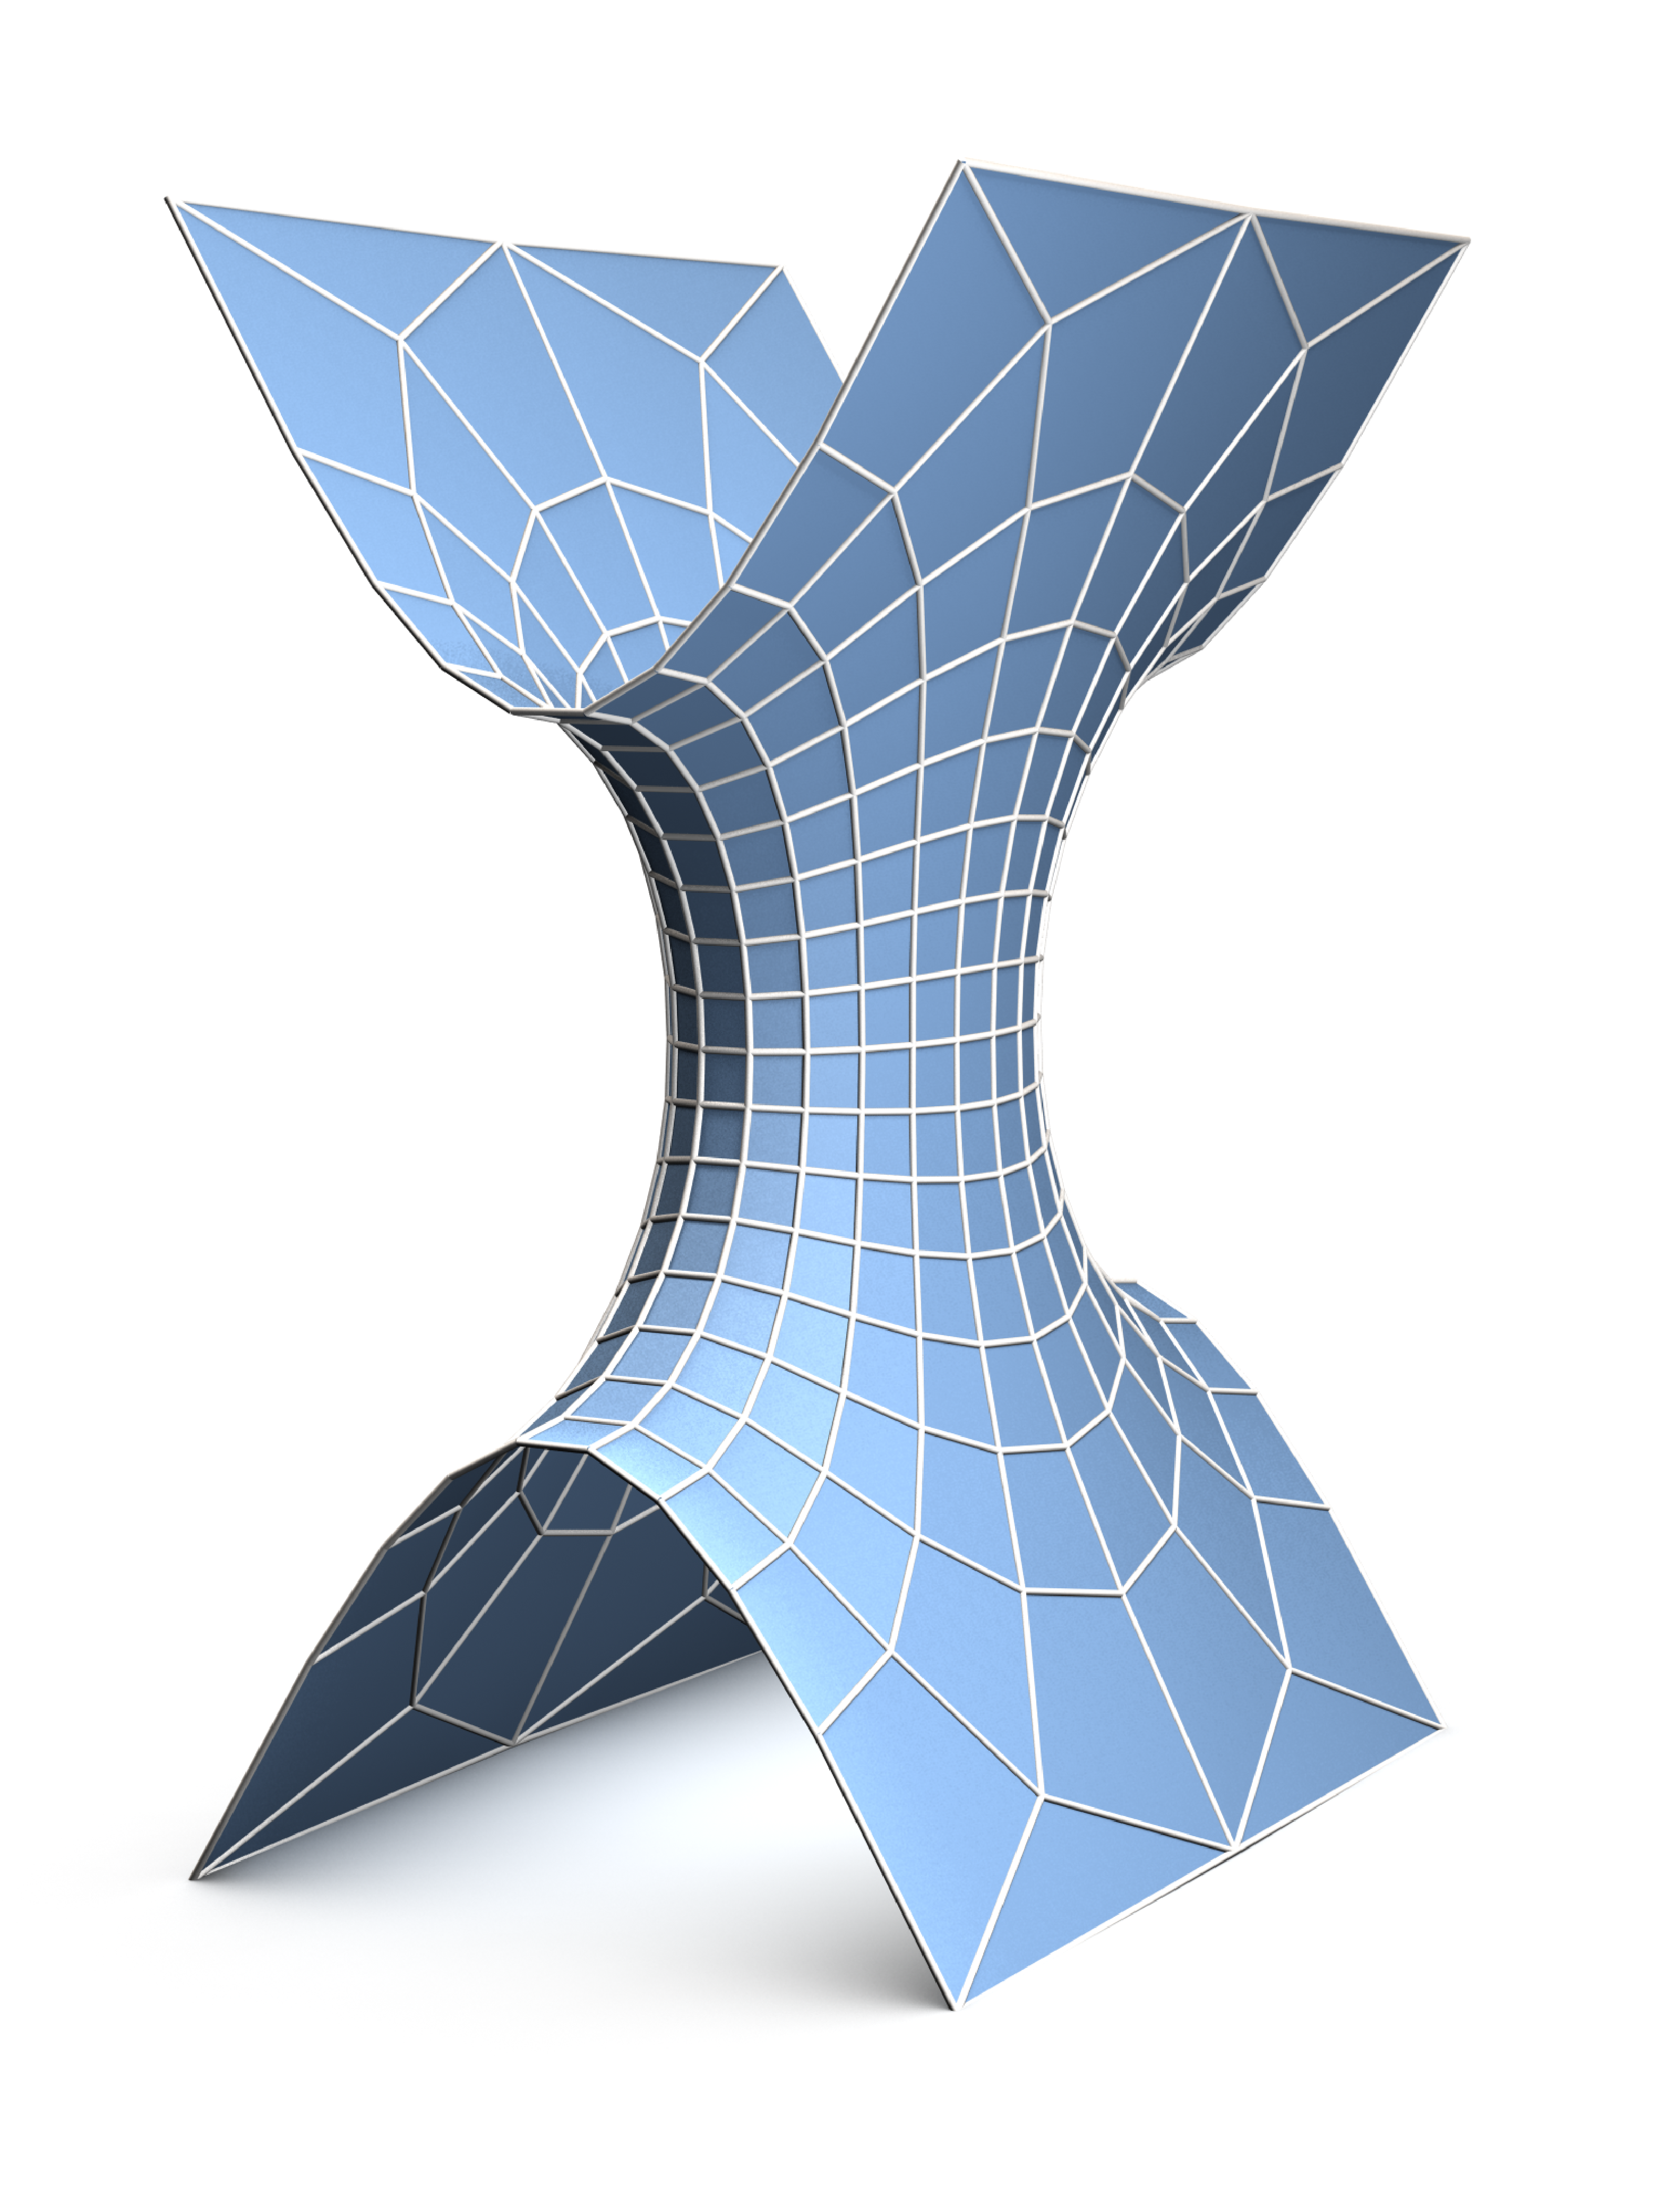
\includegraphics[height=10cm]{image/ellipsoid01_dual.pdf}
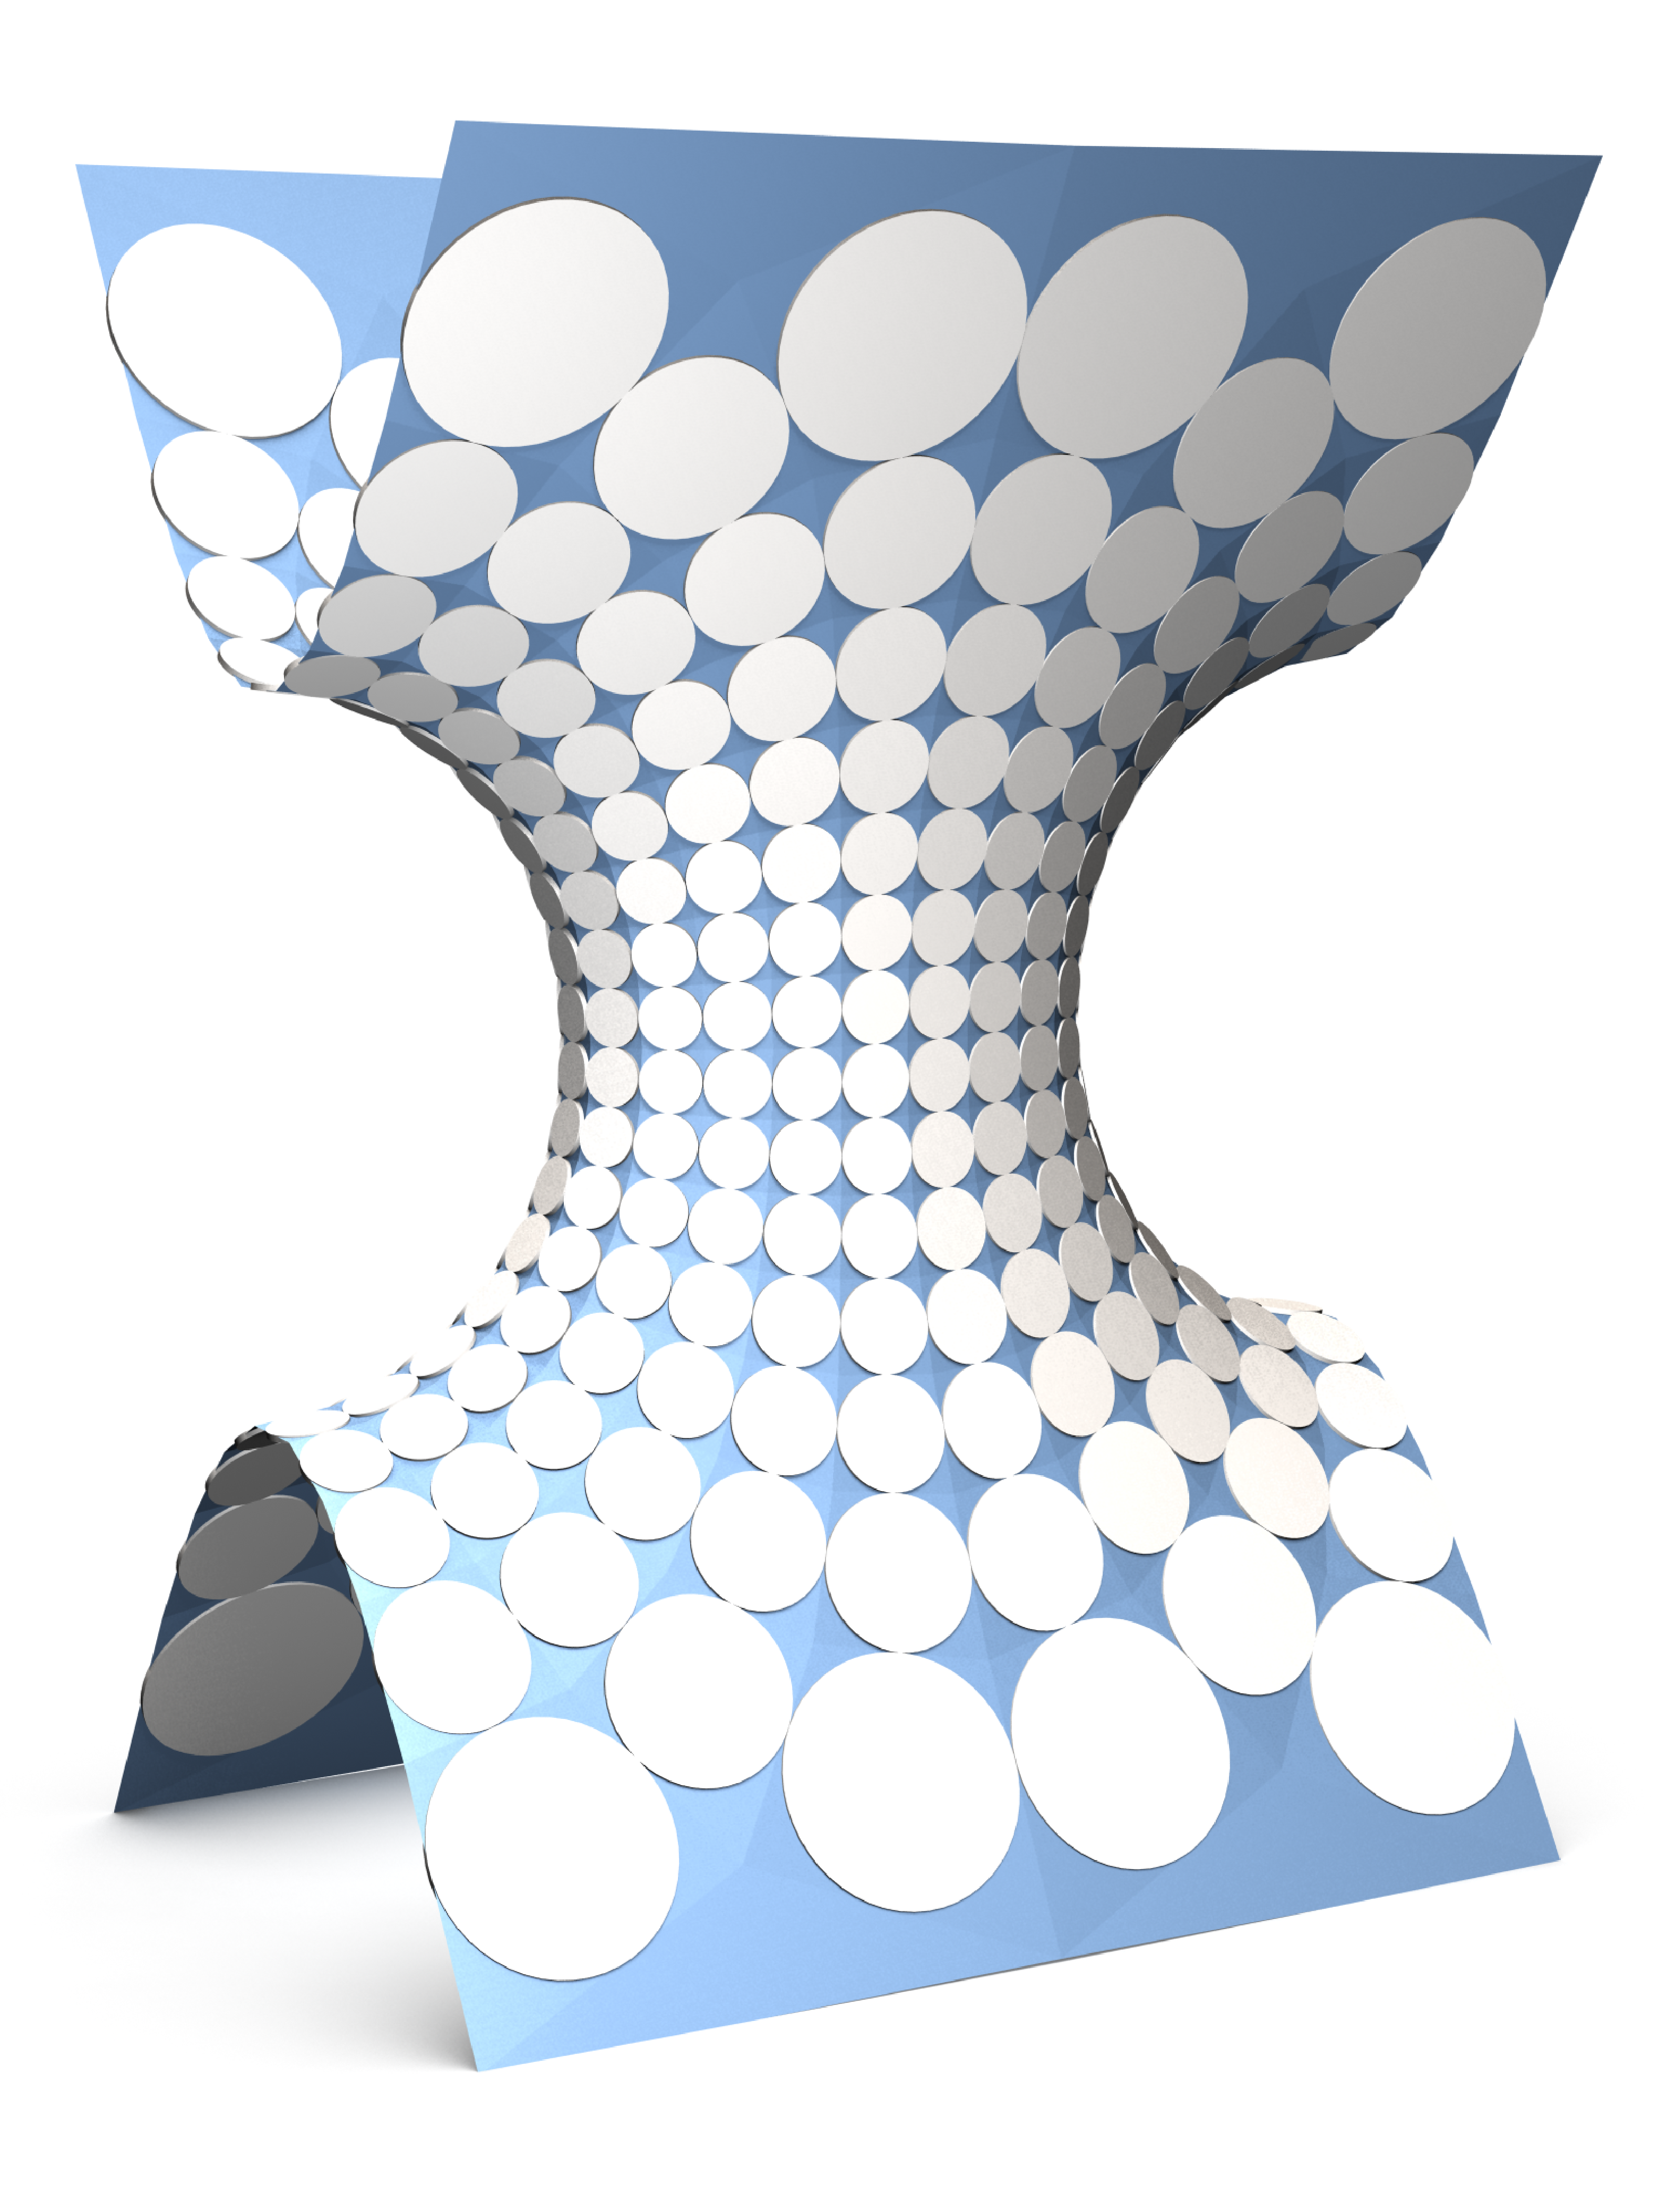
\includegraphics[height=10cm]{image/ellipsoid01_dual_disks.pdf}
}
\caption{Dual surface of discrete s-isothermic ellipsoid of Figure~\ref{fig:ellipsoid}. }
\label{fig:ellipsoid_dual} 
\end{figure}

Here we describe the construction of a discrete s-isothermic ellipsoid and 
its dual surface. (See Hertrich-Jeromin~\cite[p.~202]{Hertrich2003} for the smooth analog).
The rough construction outline is as follows. We start with a discretized version
of the smooth isothermically parameterized ellipsoid. We obtain this by calculating a 
quasiisothermic parameterization of half of a triangulated ellipsoid. After remeshing, 
the parameter lines are approximate curvature lines. We complete the surface by reflection
at the boundary. 
Optimization of the s-isothermic functional yields the final discrete ellipsoid. Its 
dual surface is constructed as in Section~\ref{sub:isometric}.

The connectivity at singularities of the discrete ellipsoid is not unique. If there is a discrete 
curvature line in the symmetry plane of the ellipsoid, we have degenerate quads that have 
vertices with angle $\approx\pi$. The singularity is located at this valence $2$ vertex. 
If there is no discrete curvature line at the symmetry plane then the singularity is located at the 
mid point of the edge connecting two valence three vertices. We have observed that 
the convergence behavior of the s-isothermic functional is considerable better in the former 
model of singularities. We therefore like to call only the discrete ellipsoid with curvature 
lines at symmetry planes a discrete ellipsoid, see Figure~\ref{fig:ellipsoid} and~\ref{fig:ellipsoid_dual}.



\section{Conclusions and future research}
\label{sec:future}
The main contributions of this article are, on the one hand, the definition of 
quasiisothermic parameterizations together with a new algorithm to
compute parameterizations of surfaces that optimizes the corresponding quality measure.
On the other hand, we have defined a new energy for meshes with touching incircles.

We see the main advantage of the algorithm presented in
Section~\ref{sec:parametrization} in its simplicity and its applicability to
shell-like roof structures which arise in architectural models. Since these
models often have almost constant mean curvature and thus allow for an almost
isothermic parameterization, our algorithm performs particularly well on these
examples.

The new energy described in Section~\ref{sec:s-isothermic} is closely related
to the work of Schiftner~\emph{et~al.}~\cite{SchiftnerHWP2009} dealing with
circle packing meshes. They explicitly do not treat quadrilateral meshes since
they are aware of the shape restrictions and focus on triangle meshes instead.
The shape restriction lies in the core of isothermic surfaces but
did not influence our results dramatically for the surfaces in our focus. How
to approximate arbitrary surfaces by isothermic surfaces is unknown and will be
subject to future research. The results of Section~\ref{sec:s-isothermic}
suggest that this might be possible using related methods.

Our new functional generates quad circle packing meshes in the sense of
Schiftner and co-authors. For surfaces arising in architectural context (in
particular for shell-like roofs) we are able to construct aesthetically
pleasing quad meshes supporting a circle packing. 

\subfilebibliography
\end{document}

%%% Local Variables:
%%% TeX-master: "Thesis.tex"
%%% End:

%!TEX root = ./Thesis.tex
\section[Projective interpolation for arbitrary parameterizations] % for the table of contents
{Projective interpolation for arbitrary parameterizations % normal title
\sectionmark{Projective interpolation} % title on the first page header of section
}
\sectionmark{Projective interpolation} % on other page headers of the sectioin

Let $M=(V, E, F)$ be a triangulated surface consisting of vertices $i\in V$, edges $\it{ij}\in E$ and faces
$\it{ijk}\in F$.



\subsection{Approximation by conformal deformation}
\subsection{Examples}

%%% Local Variables:
%%% TeX-master: "Thesis.tex"
%%% End:
%!TEX root = ./Thesis.tex

\section{A variational principle for discrete Tschebyshev nets}

Introduction...

\subsection{Variational principle}

Let $M=(V,E,F)$ be a quad-mesh. The vertices of $M$ are denoted by $v_i \in V$, the edges
are $e_{\mathrm{\it{ij}}} \in E$, and the quadrilaterals are denoted by $f_{\mathrm{\it{ijkm}}} \in F$.
\subsection{Energies}
We use a linear combination of energies to enforce desired properties on the optimised mesh.
Our energy consists of three parts.
\begin{equation}
	E(M) =	\lambda_1 E_{\textrm{\scriptsize{ref}}} + 
		\lambda_2 E_{\textrm{\scriptsize{len}}} +
		\lambda_3 E_{\textrm{\scriptsize{cur}}}
	\label{eq:energy_combination}
\end{equation}
The energy $E_{\textrm{\scriptsize{ref}}}$ penalises the distance of vertices from a
reference surface. This surface can be anything that gives a distance function, e.g., a
triangulated surface or a \textsc{Nurbs}-surface. The energy and its gradient are given 
by
\begin{eqnarray*}
	E_{\textrm{\scriptsize{ref}}}(M) &=& 
	\sum_{v_i \in V}\left<v_i - cp_i, v_i - cp_i\right> \\
	\frac{\partial E_\textrm{\scriptsize{ref}}}{\partial v_i} &=&
	2\left(v_i - cp_i\right)
	\label{eq:energy_reference}
\end{eqnarray*}
Here $v_i$ is a vertex of the optimised quad-mesh and $cp_i$ a closest point on the reference
surface measured from vertex $v_i$. The functional $E_{\textrm{\scriptsize{len}}}$ measures
edge length deviation from a given reference length $L$. Its derivative and energy is given as
\begin{eqnarray*}
	E_{\textrm{\scriptsize{len}}}(M) &=& 
	\sum_{e_{\mathrm{\it{ij}}} \in E} \left(\Vert v_i - v_j \Vert - L\right)^2\\
	\frac{\partial E_\textrm{\scriptsize{len}}}{\partial v_i} &=& 
	\sum_{e_{\mathrm{\it{ij}}} \in \textrm{\scriptsize{star}}(v_i)}
	\left(2 - \frac{2L}{\Vert v_i - v_k \Vert}\right)\left(v_i - v_k \right)
\end{eqnarray*}
The sum in the derivative is taken over all edges incident to vertex $v_i$, called the 
edge-star of vertex $v_i$. The third energy is a fairing term that penalises a notion of
curvature of curves on the surface. As we only deal with quad-meshes with $\mathbb Z^2$ combinatorics every interor vertex has four adjacent edges. The energy $E_{\textrm{\scriptsize{cur}}}$ and its gradient is defined as:
\begin{eqnarray*}
	E_{\textrm{\scriptsize{cur}}}(M) &=& \sum_{v_i\in V} \left(\pi - \angle(e_{\mathrm{\it{i1}}}, e_{\mathrm{\it{i3}}}) \right)^2 
	+ \left(\pi - \angle(e_{\mathrm{\it{i2}}}, e_{\mathrm{\it{i4}}}) \right)^2 \\
	\frac{\partial}{\partial v_j}\angle(e_{\mathrm{\it{ij}}},e_{\mathrm{\it{ik}}}) &=& 
	\frac{-1}{\left\Vert e_{\mathrm{\it{ij}}}\right\Vert}\left(e_{\mathrm{\it{ik}}}-e_{\mathrm{\it{ij}}}\frac{\left<e_{\mathrm{\it{ik}}},e_{\mathrm{\it{ij}}}\right>}{\left<e_{\mathrm{\it{ij}}},e_{\mathrm{\it{ij}}}\right>}\right)
	\left\Vert e_{\mathrm{\it{ik}}}-e_{\mathrm{\it{ij}}}\frac{\left<e_{\mathrm{\it{ik}}},e_{\mathrm{\it{ij}}}\right>}		
	{\left<e_{\mathrm{\it{ij}}},e_{\mathrm{\it{ij}}}\right>} \right\Vert^{-1} \\
	\frac{\partial}{\partial v_i}\angle(e_{\mathrm{\it{ij}}},e_{\mathrm{\it{ik}}}) &=& 
	- \left(\frac{\partial}{\partial v_j}\angle(e_{\mathrm{\it{ij}}},e_{\mathrm{\it{ik}}}) + 
	\frac{\partial}{\partial v_k}\angle(e_{\mathrm{\it{ij}}},e_{\mathrm{\it{ik}}})\right)
\end{eqnarray*}
Here and $e_{\mathrm{\it{i1}}}$, $e_{\mathrm{\it{i2}}}$, $e_{\mathrm{\it{i3}}}$, and $e_{\mathrm{\it{i4}}}$ are the adjacent edges of $v_i$ in cyclic order. An edge $e_{\mathrm{\it{ij}}}$ is also used in the role of a vector pointing from vertex $v_i$ to vertex $v_j$. $\angle(e_{\mathrm{\it{ij}}},e_{\mathrm{\it{ik}}})$ is the angle spaned by the vectors $e_{\mathrm{\it{ij}}}$ and $e_{\mathrm{\it{ik}}}$  From the angle derivatives with respect to the vertices the gradient can be computed efficiently.

\begin{figure}[ht]
\centering
\resizebox{\textwidth}{!}{
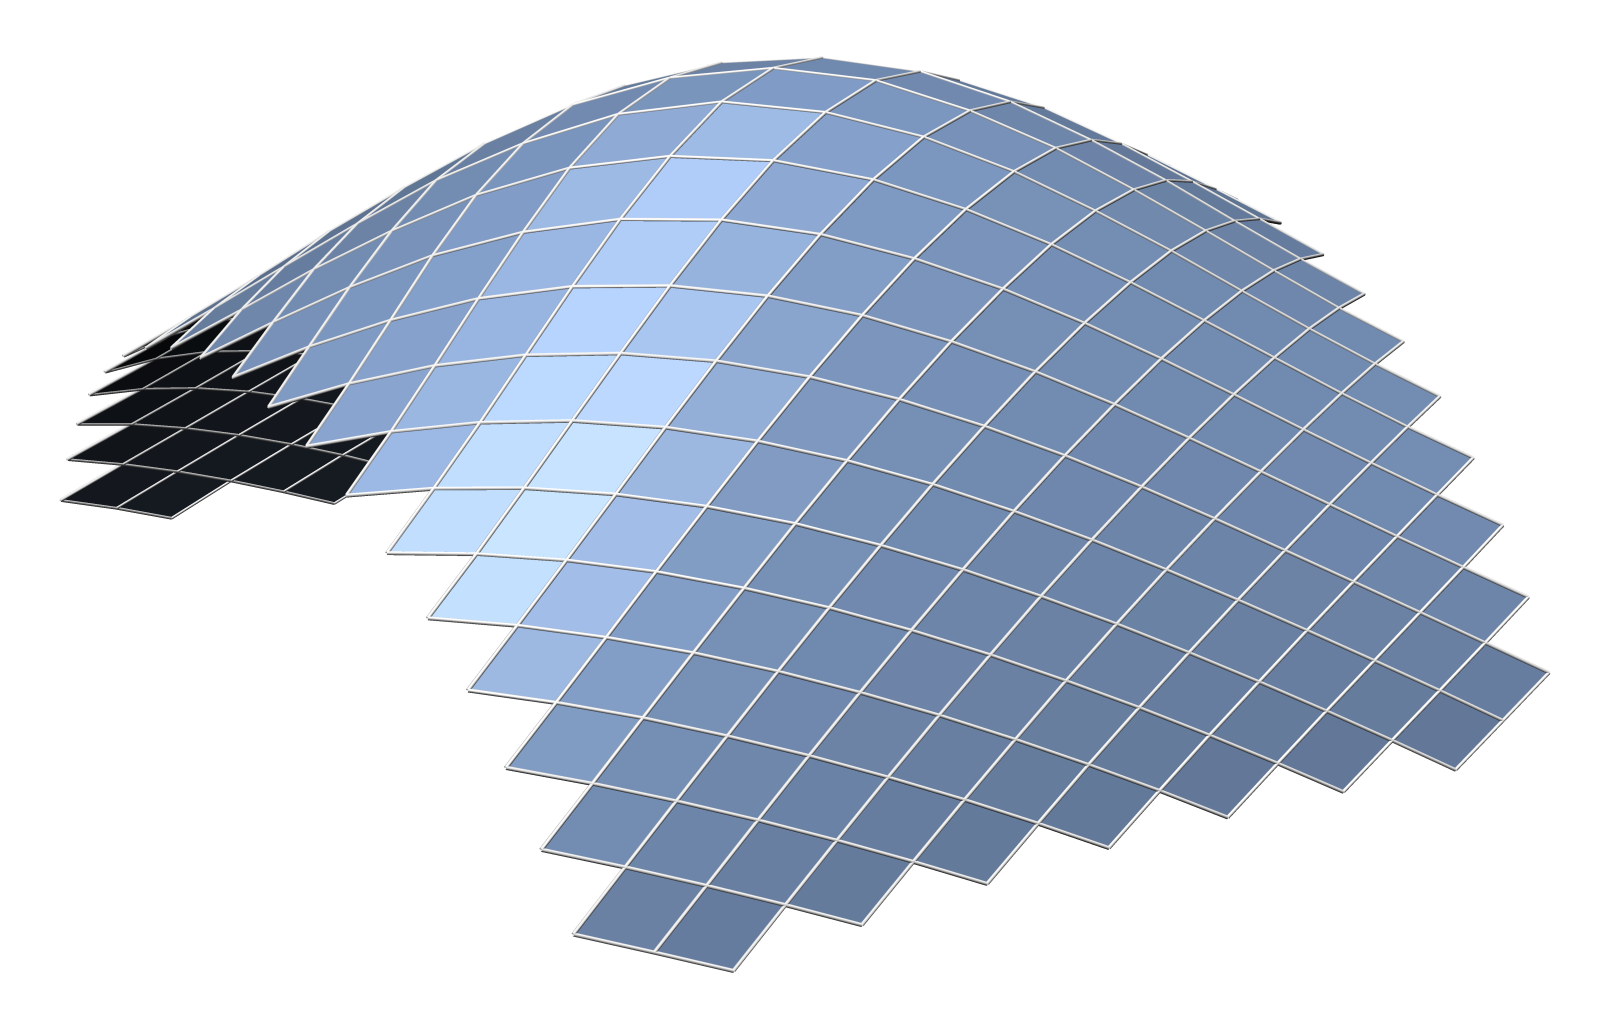
\includegraphics[width=0.33\linewidth]{image/tscheby/init60_mesh.png}
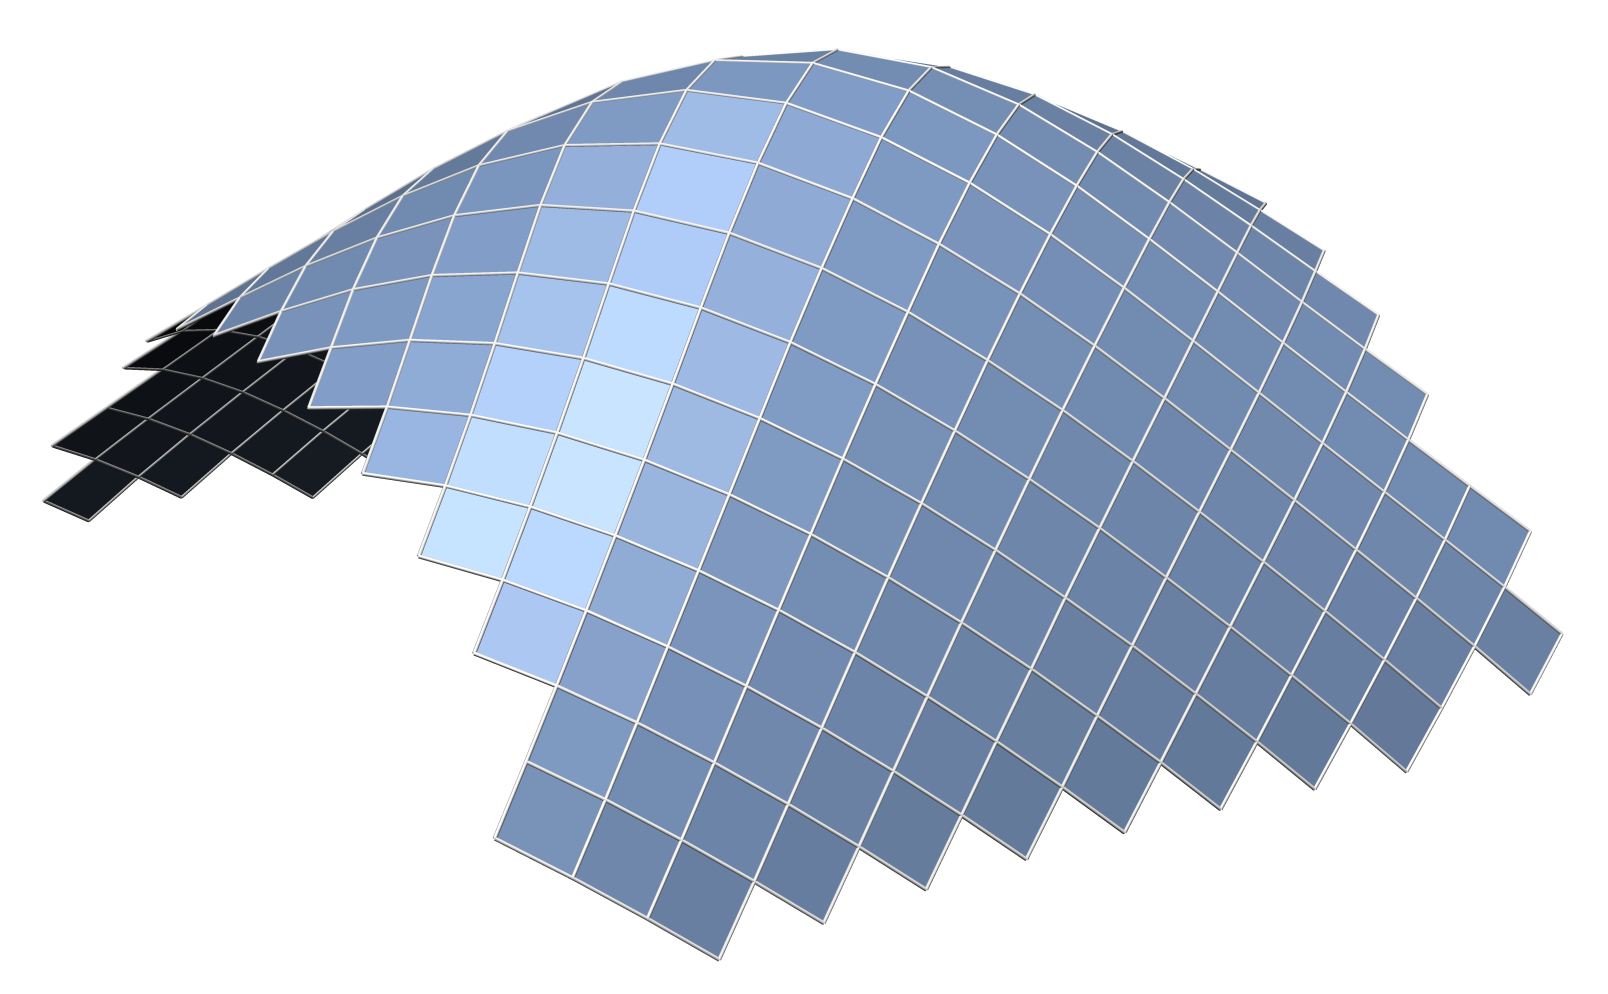
\includegraphics[width=0.33\linewidth]{image/tscheby/init90_mesh.png}
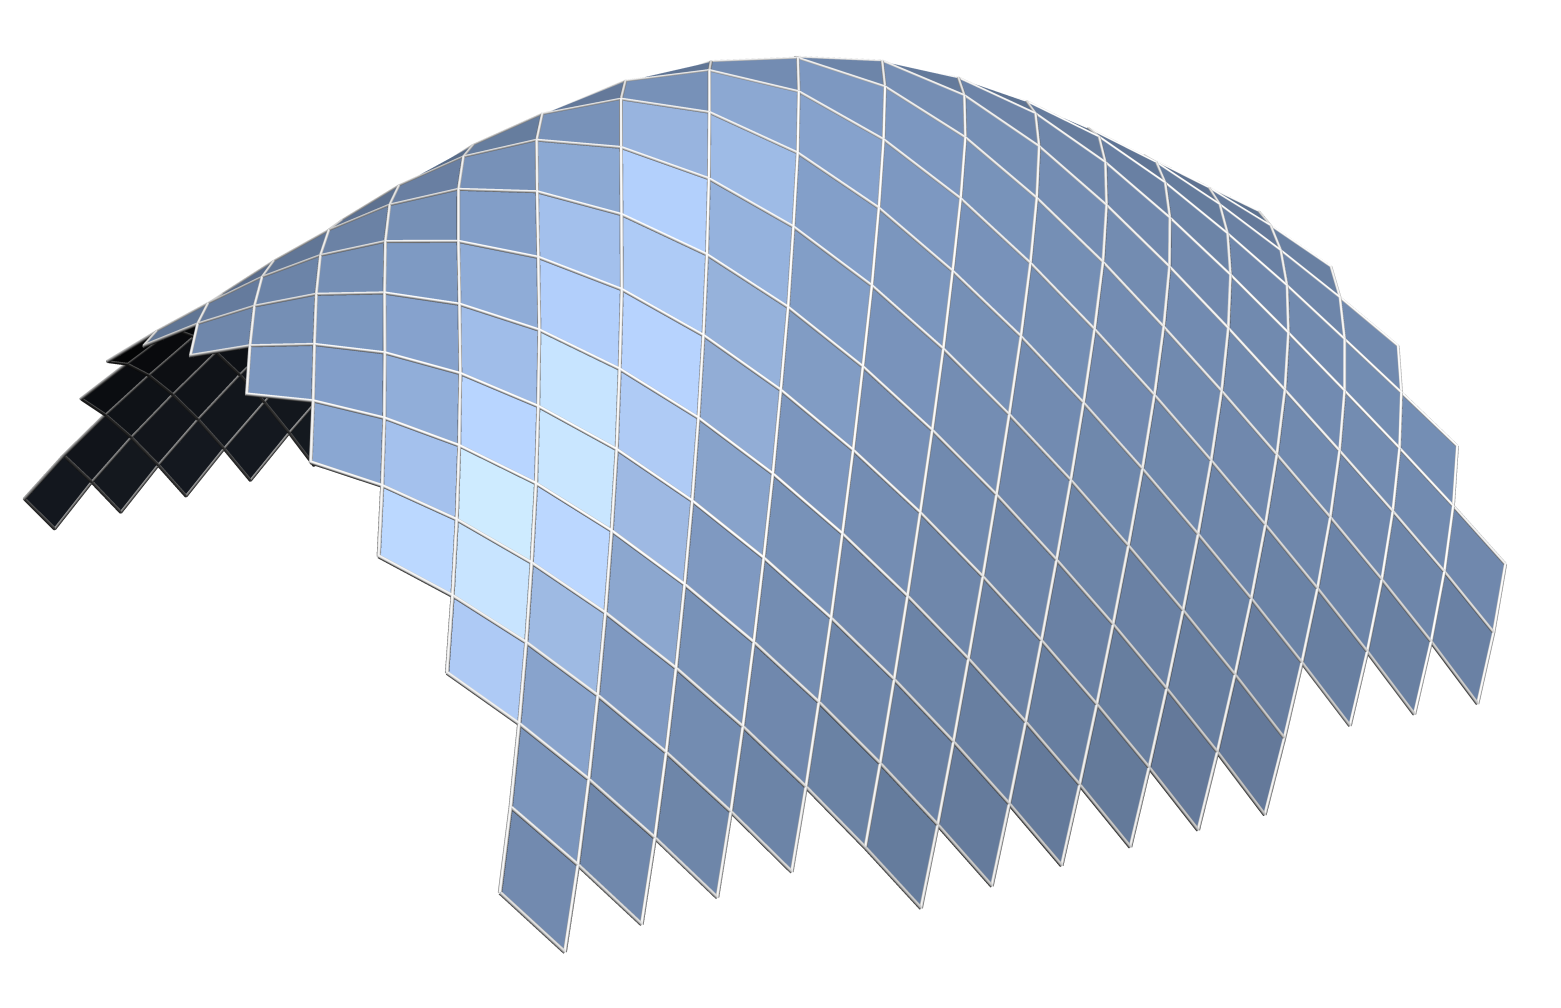
\includegraphics[width=0.33\linewidth]{image/tscheby/init120_mesh.png}
}
\caption{Different initialization shear angles for a conformal remesh. $30^\circ$ left, $0^\circ$ middle, and $-30^\circ$ right.}
\label{fig:initial_grids}
\end{figure}
\subsection{Initialization and parameters}
The energy $E(M)$ is in general non-convex. That means there can be many local optima, and the solution found by some gradient descent depends on the initialisation. We propose to use a conformal remesh of the reference surface as initialization. The conformality of the parameterisation gives us control over the angles between edges of the quadrilaterals. We can introduce shear to the parameterisation and modify this angle globally. By this we start with meshes that have almost constant edge angle (see Fig.~\ref{fig:initial_grids}).

\subsection{Implementation}
We use the conformal mapping algorithm by \cite{Springborn2008} to create the
initial mesh. To minimize the energy $E(M)$ we use the non-linear optimization package
PETSc/TAO \cite{petsc-web-page,tao-user-ref} and its java binding 
\cite{jpetsctao-web-page}. We have made good experiences with normalising the
 energies to have gradient length one before optimization. Then we start with all
$\lambda$s equal to one and modify them on the way if needed. If one encounters
degenerate configurations during optimization one can drop the length energy term for 
a few iterations.

%%% Local Variables:
%%% TeX-master: "Thesis.tex"
%%% End:
\part{Software Packages}
\documentclass[Thesis.tex]{subfiles}
\begin{document}
\setkeys{Gin}{draft=false}
\chapter{Introduction}

In this chapter words printed in {\sc SmallCapitals} are names of software packages, words printed
in {\tt TeleType} are names of {\sc Java} classes, methods, or fields.

\section{Mathematical Software Development}

\begin{figure}[h]
	\centering
	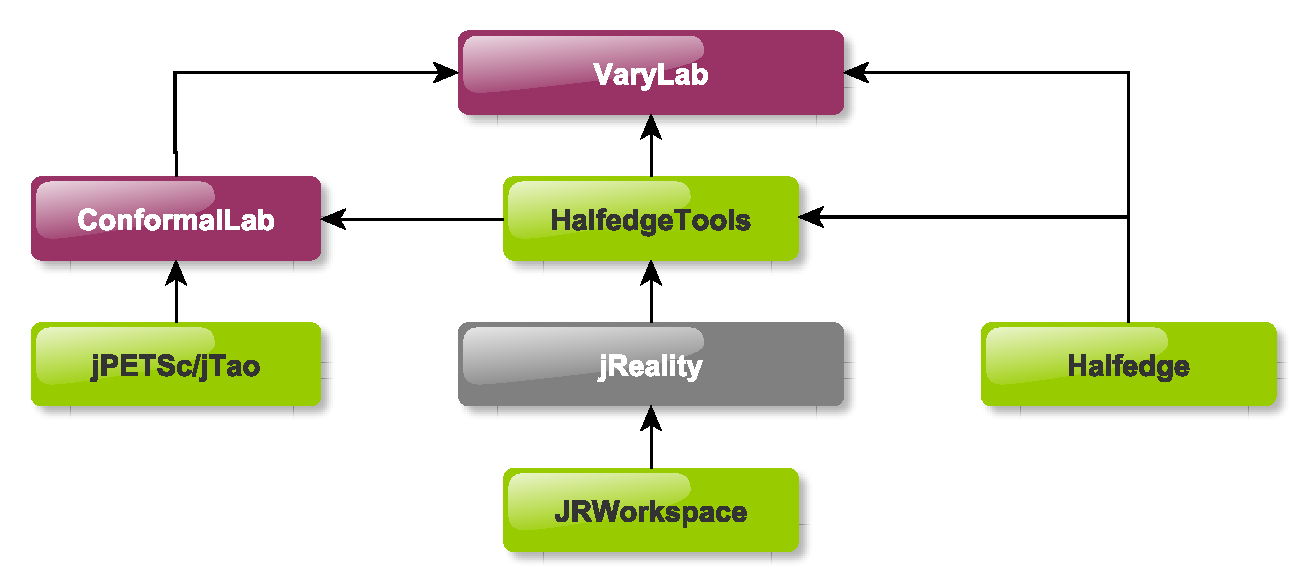
\includegraphics[width=\linewidth]{figures/software_architecture}
	\caption[Software package dependencies]{
		Software architecture and dependencies of the DDG Framework. 
		{\sc Jtem} library packages (green), application packages (blue). {\sc JReality} is used mainly for 3d-visualization (grey).}
	\label{fig:software_architecture}
\end{figure}

In the field of Discrete Differential Geometry (DDG) there is a special need for experiments
with the help of computer software. Especially if the methods of DDG are applied
to problems in computer graphics, geometry processing, or architecture, algorithms have 
to be implemented and convincing examples have to be presented. Additionally, a suitable 
visualization of the results has to be included in a state-of-the-art publication.

There is a growing knowledge of software development in the mathematical community. This 
is party due to the curricula of universities which started to include programming courses for 
undergraduate students with a visualization emphasis, e.g., \cite{VisMathHomepage, 
CaltechVisMath}. This knowledge enables students to extend their abilities of creating visualizations and 
mathematical software, where former generations of students solely used the visualization 
abilities of standard computer algebra packages like Mathematica or MatLab.

The audience of this chapter is two-fold. On the one hand it is students creating their 
visualizations of surfaces and develop algorithms. On the other hand it is researchers in the
field of discrete differential geometry who need a stable data structure and programming
infrastructure to get the job done.

This part of the thesis is the description and getting-started manual of a set of software packages
(Berlin DDG Framework) written in the programming language {\sc Java}. They are 
specifically designed for the creation of custom interactive software for experiments with algorithms and geometries treated within DDG. It is currently beeing used for teaching mathematical visualization courses at TU-Berlin \cite{VisMathHomepage} and for research projects within the geometry group.

%Section~\ref{sec:related_work} gives an overview of existing software packages that have a focus similar to the DDG Framework. 
Chapter~\ref{chp:jrworkspace} introduces the {\sc JRworkspace} library of the 
{\sc Jtem} project~\cite{JtemWebsite}. It is the foundation of any application created with 
the DDG Framework. It is also the user interface basis of {\sc Jreality}, a mathematical 
visualization library that uses {\sc JRworkspace} as plug-in and user interface 
tool~\cite{JrealityWebsite}. Chapter~\ref{chp:halfedge} introduces the 
{\sc HalfEdge} and {\sc HalfEdgeTools} package. They implement half-edge data 
structure and various user interface tools and algorithms for interaction and editing.  
In Chapter~\ref{chp:conformallab} we describe the software 
{\sc ConformalLab}. This package implements the methods of the 
publications~\cite{Bobenko2010, OWR2012, Sechelmann2012, BobSechSpr}.
Chapter~\ref{chp:varylab} introduces {\sc VaryLab}, the software implementation of the 
methods described in the publications \cite{Lafuente2011, Lafuente2012, Sechelmann2012}.
This package is also released to partners of the development group as {\sc VaryLab[Gridshells]},
{\sc VaryLab[Ultimate]}, or even online as {\sc VaryLab[Service]}\cite{varylab-web-page}.

Figure~\ref{fig:software_architecture} shows the dependencies of the packages. Every
application depends on {\sc JRworkspace} which implements plug-in functionality. It is
the basis of the {\sc Jreality} plug-in system. {\sc Half\-Edge\-Tools} is using {\sc Jreality} 
for visualization and is build on top of the {\sc Jtem} project {\sc Half\-Edge}. 
{\sc ConformalLab} and {\sc VaryLab} use {\sc Jpetsc/Jtao} to perform numerical
optimization. Their algorithms are implemented as {\sc JRworkspace} plug-ins.

The development of the described software is joint work with Thilo R{\" o}rig 
({\sc HalfEdgeTools, VaryLab}), the {\sc Jreality} members~\cite{JrealityWebsite}, Hannes 
Sommer ({\sc Jpetsc/Jtao})~\cite{jpetsctao-web-page}, Ulrich Pinkall and Paul Peters 
({\sc JRworkspace}), and Boris Springborn ({\sc Halfedge}).

%
%\section{Related Work}
%\label{sec:related_work}
%There are many mathematically oriented software frameworks available to the community. So why adding a new one to the list? The answer lies in the history of the software. 
%JavaView, CGAL, libIGL, ...
%Do I really want to write about this here??
%
%\subsubsection{JavaView} JavaView, see \cite{javaview}, is 3d geometry visualization software. It has a strong focus on web presentation as {\sc Java} applet.
%
%\subsubsection{libigl} C++ 


\chapter{{\sc JRworkspace} - Java API for modular applications}
\label{chp:jrworkspace}

%\begin{figure}
%	\centering
%	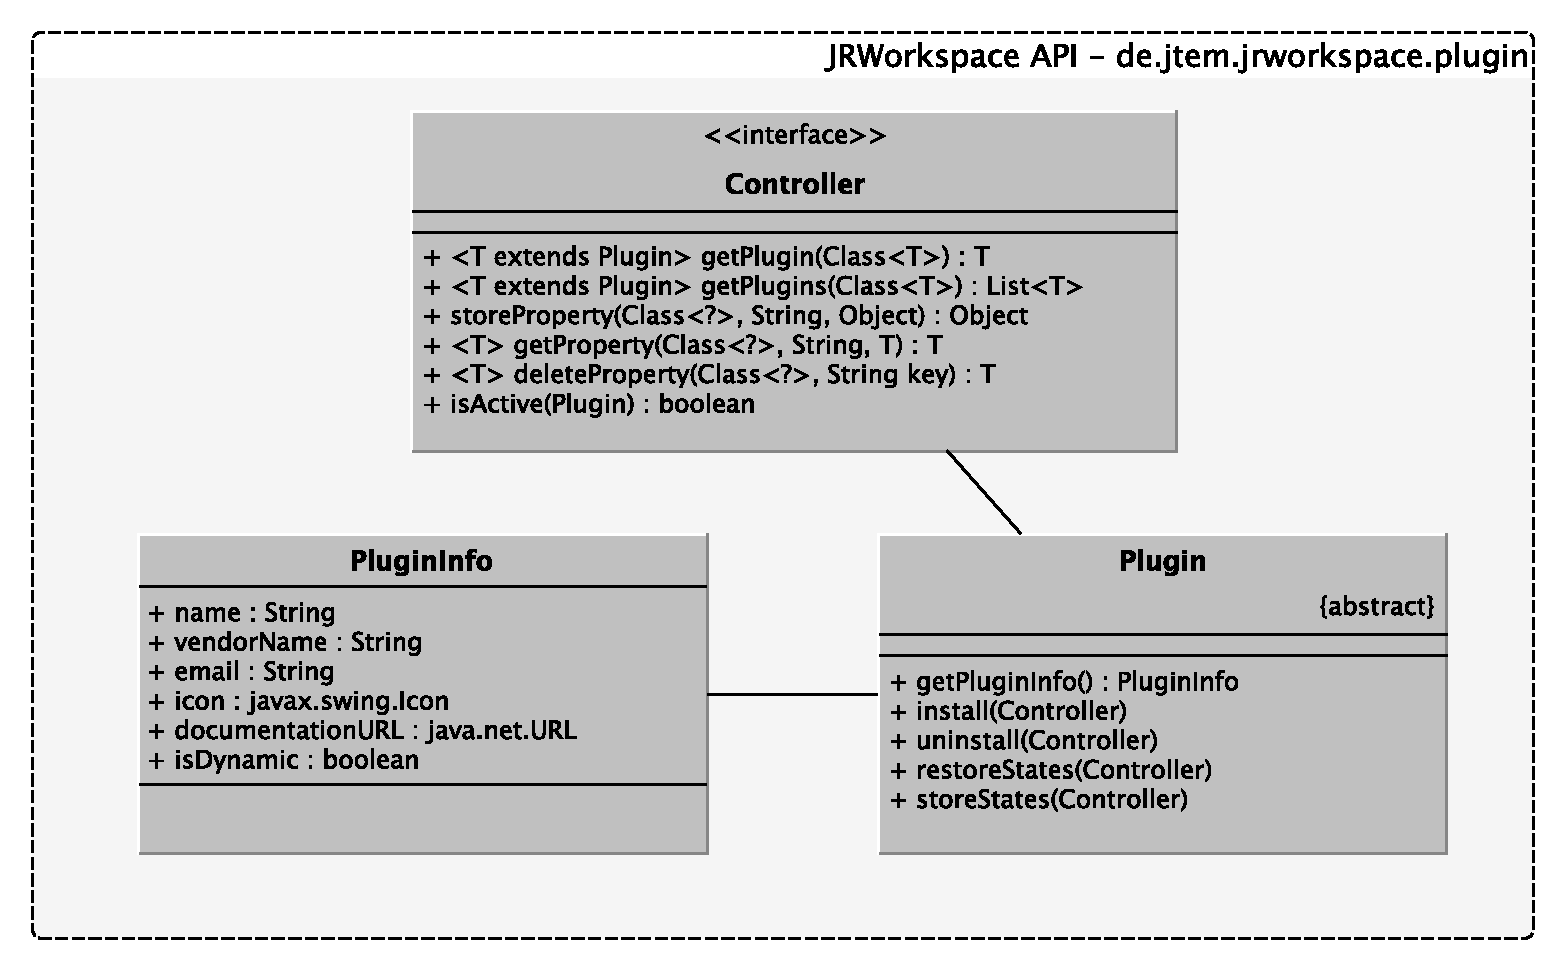
\includegraphics[width=0.8\linewidth]{figures/jrworkspace_uml}
%	\caption[{\sc JRworkspace} API]{
%		UML diagram for the {\sc JRworkspace} API.
%	}
%	\label{fig:jrworkspace_uml}
%\end{figure}

{\sc JRworkspace} is part of the {\sc Jtem} family of software projects 
\cite{JtemWebsite}. It defines a simple API to create modular Java applications. This API consists of
three basic classes (Listings~\ref{lst:plugin_base}, \ref{lst:controller_interface}, and 
\ref{lst:plugin_info}).
The project contains a reference implementation that supports the creation of Java
Swing applications using the {\sc JRworkspace} API. This implementation is used in all 
applications described in this work.

\section{Plug-ins and the controller}
\label{sec:plugins}

In a {\sc JRworkspace} application a feature is implemented as plug-in and the corresponding Java class 
extends the abstract class Plugin
(Listing~\ref{lst:plugin_base}). The idea is that a plug-in can be installed by the controller 
calling its {\tt install} method or uninstalled via the {\tt uninstall} method. You can think of it 
as a feature added to your program. In particular there is no more than one instance of a
plug-in class in a {\sc JRworkspace} application.

A plug-in has a life-cycle during the runtime of the program which includes these basic
steps:
\begin{center}
\begin{tabular}{r|r|l}
	instantiation & 1 & set default plug-in state\\
	{\tt restoreStates} & 2 & load plug-in state from {\tt Controller}\\
	{\tt install} & 3 & calls {\tt getPlugin} to obtain dependent plug-ins\\
	{\tt --}  & 4 & program execution\\
	{\tt storeStates} & 5 & stores state values to the {\tt Controller}\\
	({\tt uninstall} & 6 & clean up)
\end{tabular}
\end{center}
Step 1 instantiates a plugin and initializes its default properties. In step 2 the controller 
calles the {\tt restoreStates} method. Step 3 is the actual installation of the plug-in. 
During runtime
of the application the plug-in can interact with possible user interface it created during 
installation or offer services to other plug-ins. 
Before program termination or before uninstall the {\tt storeStates} method is called. The plug-in
is supposed to store its state values by calling the {\tt storeProperty}
method of the controller.
Inter-plug-in-communication is done via the {\tt getPlugin} method of the controller. 
A plug-in should call {\tt getPlugin} from within the {\tt install} method to obtain the unique instance 
of a dependent plug-in. The {\tt getPlugin} method always returns the same instance of a plug-in so its
result can be stored by the {\tt install} method for later reference, see for example 
Listing~\ref{lst:sample_plugin}. Step 6 {\tt uninstall} is only used with dynamic plug-ins that support 
this operation. An implementation of {\tt Controller} may not support uninstallation of plug-ins.

We describe the basic API usage from a programmers point of view by giving an example plug-in
in Listing~\ref{lst:sample_plugin} and the source code of the three basic API classes 
{\tt Plugin}, {\tt Controller}, and {\tt PluginInfo} in Listings~\ref{lst:plugin_base}, 
\ref{lst:controller_interface}, and \ref{lst:plugin_info}.

\lstinputlisting[
	caption={
A simple plug-in class. It depends on a plug-in called {\tt DependentPlugin} 
and has the property {\tt doubleState}. It provides the method {\tt helloPlugin()} that 
prints some message. In the {\tt storeStates} method the value of {\tt doubleState} is
written to the controller. The class {\tt MyPlugin} is used as context class. The name of 
this class is used as name space to avoid property name ambiguities. The value of {\tt doubleState}
is read from the controller in the {\tt restoreStates} method using the same context class and
property name as in {\tt storeStates}. If there is no value with the given context and name
the default value {\tt 1.0} is returned by the {\tt getProperty} method. 
	},
	label=lst:sample_plugin,
	captionpos=b,
	firstline=6
] {java/de/sechel/thesis/MyPlugin.java}

\lstinputlisting[
	caption={
The {\tt Plugin} base class (excerpt). Note that plug-ins are equal if their classes are. 
It is not supported to have multiple instances of the same plug-in class installed.
	},
	label=lst:plugin_base,
	captionpos=b,
	firstline=3,
	lastline=30
] {java/de/jtem/jrworkspace/plugin/Plugin.java}

\lstinputlisting[
	caption={
The {\tt Controller} interface. A plug-in can obtain other plug-in instances by calling 
{\tt getPlugin} which returns a unique instance of the given plug-in class. The semantics
of the {\tt getPlugins} methods is different. It returns all plug-ins that are already known 
to the controller so no new dependencies are created by calling {\tt getPlugins}. Property
handling is done via the {\tt xxProperty} methods. Note that any {\tt Object} can be used
as property value. This requires the controller to use generic serialization to store data. It is 
strongly discouraged to use other classes than official java API classes as stored values as 
deserialization may fail if class geometry changes. 
	},
	label=lst:controller_interface,
	captionpos=b,
	firstline=5
] {java/de/jtem/jrworkspace/plugin/Controller.java}

\lstinputlisting[
	caption={
The plug-in meta data class (excerpt). Instances are returned by the {\tt getPluginInfo}
method of any plug-in. The value of the {\tt name} field is a plaintext name that could be 
shown in a user interface as well are the {\tt vendorName} and {\tt email} information. An optional 
{\tt icon} and a {\tt documentationURL} can be given. The flag {\tt isDynamic} is evaluated
by controller implementations that support deinstallation of plug-ins. A dynamic plug-in can
be installed or uninstalled during application runtime. A non-dynamic plug-in must be installed
at startup and remains installed until program termination. The static {\tt create} method returns
a default {\tt PluginInfo} instance for the given plug-in class.
	},
	label=lst:plugin_info,
	captionpos=b,
	firstline=7,
%	lastline=15
] {java/de/jtem/jrworkspace/plugin/PluginInfo.java}

In the next section we describe an implementation of this API.

\section{Reference implementation - {\tt SimpleController}}
\label{sec:reference_implementation}
This section describes a reference implementation of the {\sc JRworkspace} plug-in API.
It was started as a user interface framework for {\sc Jreality}~\cite{JrealityWebsite}. It implements
the {\tt Controller} interface in a class called {\tt SimpleController}. This name is historic
and did not change as the features evolved from simple into quite complex.
{\tt SimpleController} implements a {\sc Java Swing\TReg} framework for the creation of complex
modular applications based on the {\sc JRworkspace} API. It defines various plug-in flavors
that define user interface features. The implementation does not support dynamic plug-ins.

In the remainder of this section I describe the basic and most interesting features of this 
implementation. For a complete API reference see the documentation on the {\sc Jtem} website 
\cite{JtemWebsite}.


{\bf Perspective Flavor}

A plug-in implementing the interface {\tt PerspectiveFlavor} provides the base for a program's user 
interface. It implements the method {\tt getCenterComponent} that returns a AWT {\tt Conponent}
that is placed in the main frame of the application. The main program window itself is created and
managed by the controller.
A reference implementation of this flavor is the {\tt SideContainerPerspective}. It layouts its content 
using a {\tt BorderLayout} and places slots in the north, south, east, and west of the main window. These
slots can contain {\tt ShrinkPanel}s that can be moved between slots by drag-and-drop. A {\tt ShrinkPanel}
behaves like a {\tt JPanel} and has a title bar that resizes the panel when the user clicks with the mouse.

\begin{figure}[H]
\centering
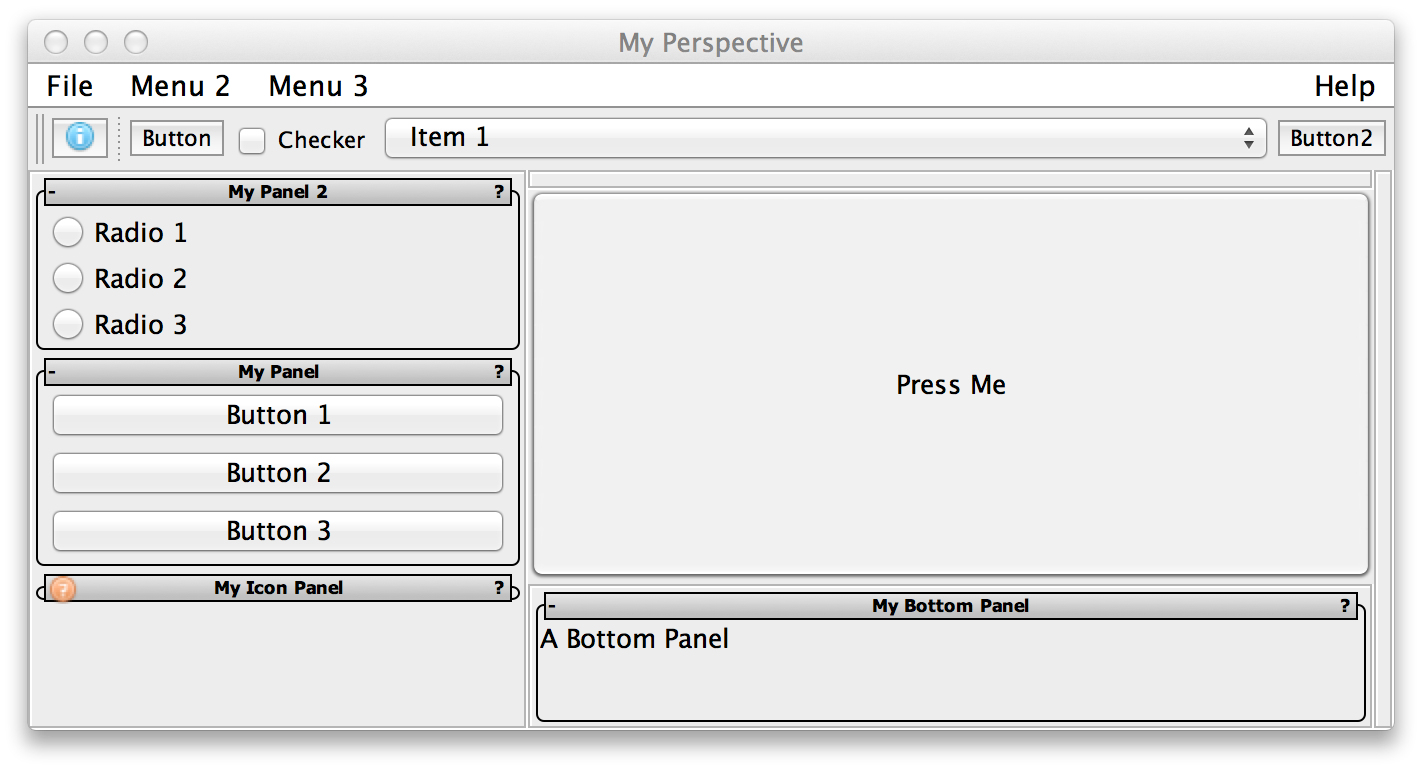
\includegraphics[width=9cm]{jrworkspace/side_containers_hires.png}
\caption[The {\tt SideContainerPerspective} user interface plug-in]{The {\tt SideContainerPerspective} implementation uses slots to layout panels at the side of the
main window. The left slot contains three {\tt ShrinkPanel}s, the top and right slots are empty. The menu bar 
and tool bar are created by respective plug-in flavors.}
\label{fig:side_containers}
\end{figure}


{\bf Menu Flavor}

A plug-in implementing the {\tt MenuFlavor} interface provides {\sc Java Swing\TReg} menu 
components that are placed at the top of the main window. A reference implementation of this
flavor is the plug-in {\tt MenuAggregator} that manages menu entries by contexts and
menu paths. Its API provides four methods to add and remove menus, menu items, and
separators. A typical method signature is

\begin{lstlisting}[numbers=none]
	public void addMenu(Class<?> ctx, double priority, JMenu m, String... path)
\end{lstlisting}

where the plug-in stores the menu item with the given context class. This context is used to
bulk-remove menus from a menu aggregator. Menus are sorted ascending
by their priority. The menu item appears at the end of the given menu path. See 
Listing~\ref{lst:menu_aggregator} and Figure~\ref{fig:menu_aggregator}.


\begin{figure}[H]
\centering
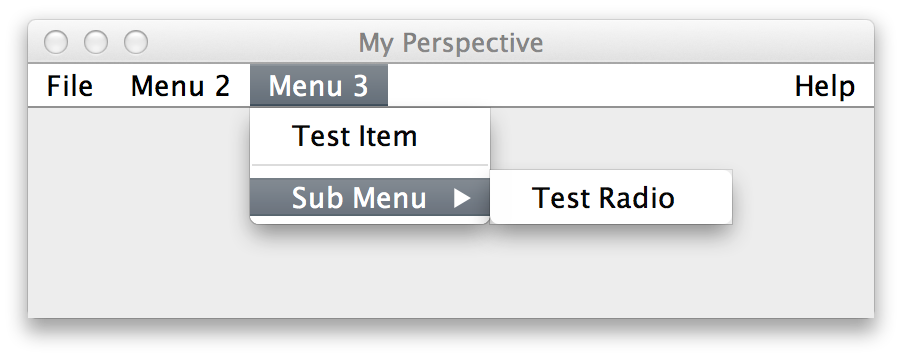
\includegraphics[width=7cm]{jrworkspace/menu_bar_hires.png}
\caption{The menu created by Listing~\ref{lst:menu_aggregator}}
\label{fig:menu_aggregator}
\end{figure}

\lstinputlisting[
	caption={Usage of the {\tt MenuFlavor} interface and the {\tt MenuAggregator} implementation.},
	label=lst:menu_aggregator,
	captionpos=b,
	firstline=40,
	lastline=51
] {java/de/sechel/thesis/MyMenuBar.java}

{\bf Tool Bar Flavor}

Plug-ins implementing this flavor interface create a {\sc Java Swing\TReg} tool bar at the top of the 
main window. There can be more than one plug-in implementing this interface to create multiple 
tool bars. The API method signatures a similar to the signatures of the menu aggregator flavor. As 
a tool bar does not have a hierarchy, there is no path parameter. The signature of a API method is, e.g.,

\begin{lstlisting}[numbers=none]
	public void addAction(Class<?> context, double priority, Action a).
\end{lstlisting}

The tool bar aggregator implementation can handle {\tt Action}s, {\tt Component}s, and tool bar
separators. See Listing~\ref{lst:tool_bar_aggregator} and Figure~\ref{fig:tool_bar_aggregator}.

\begin{figure}[H]
\centering
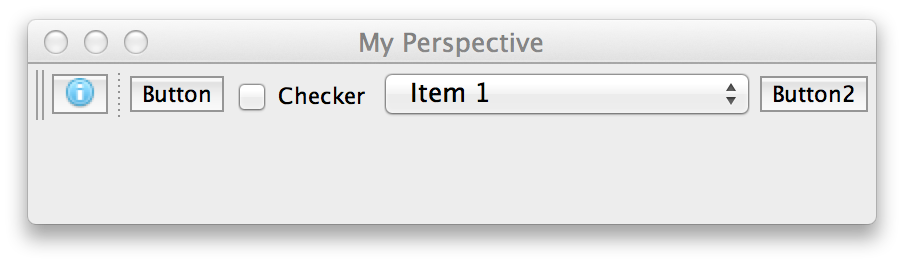
\includegraphics[width=7cm]{jrworkspace/tool_bar_hires.png}
\caption{The tool bar created by Listing~\ref{lst:tool_bar_aggregator}. Elements are sorted according to their
priority.}
\label{fig:tool_bar_aggregator}
\end{figure}

\lstinputlisting[
	caption={Usage of the {\tt ToolFlavor} interface and the {\tt ToolBarAggregator} implementation.},
	label=lst:tool_bar_aggregator,
	captionpos=b,
	firstline=40,
	lastline=50
] {java/de/sechel/thesis/MyToolBar.java}

{\bf The API of {\tt SimpleController}}

A plug-in implementation is independent of the concrete implementation of the {\tt Controller}. To create an
application with the {\tt SimpleController} we need to register plug-ins we want to use and then invoke the
startup sequence. A typical {\tt main} method is, e.g.,

\lstinputlisting[
	caption={{\tt Main} method of a program created with the {\tt SimpleController} implementation. The result
is shown in Figure~\ref{fig:side_containers}.},
	label=lst:main_method,
	captionpos=b,
	firstline=13,
	lastline=28
] {java/de/sechel/thesis/MyApplication.java}

We set the look and feel to be the system look and feel, in this case the Mac OS style. Then we create a
{\tt SimpleController} and set the {\tt magageLookAndFeel} property to {\tt false}. Plug-in properties are saved
to a file called {\tt MyApp.xml}. There are two property modes defined by the {\tt SimpleController}, {\tt StaticPropertiesFile}
and {\tt UserPropertiesFile}. In static mode there is only one file location. In user mode the predefined location can
be altered by the user of the program. This user decision is then stored as a {\sc Java} preference. In this example 
we use the static properties.

\section{{\sc JRworkspace} and {\sc Jreality}}

The user interface of {\sc Jreality} \cite{JrealityWebsite} is based on the {\sc JRworkspace} API and reference
implementation.

\begin{figure}[H]
\centering
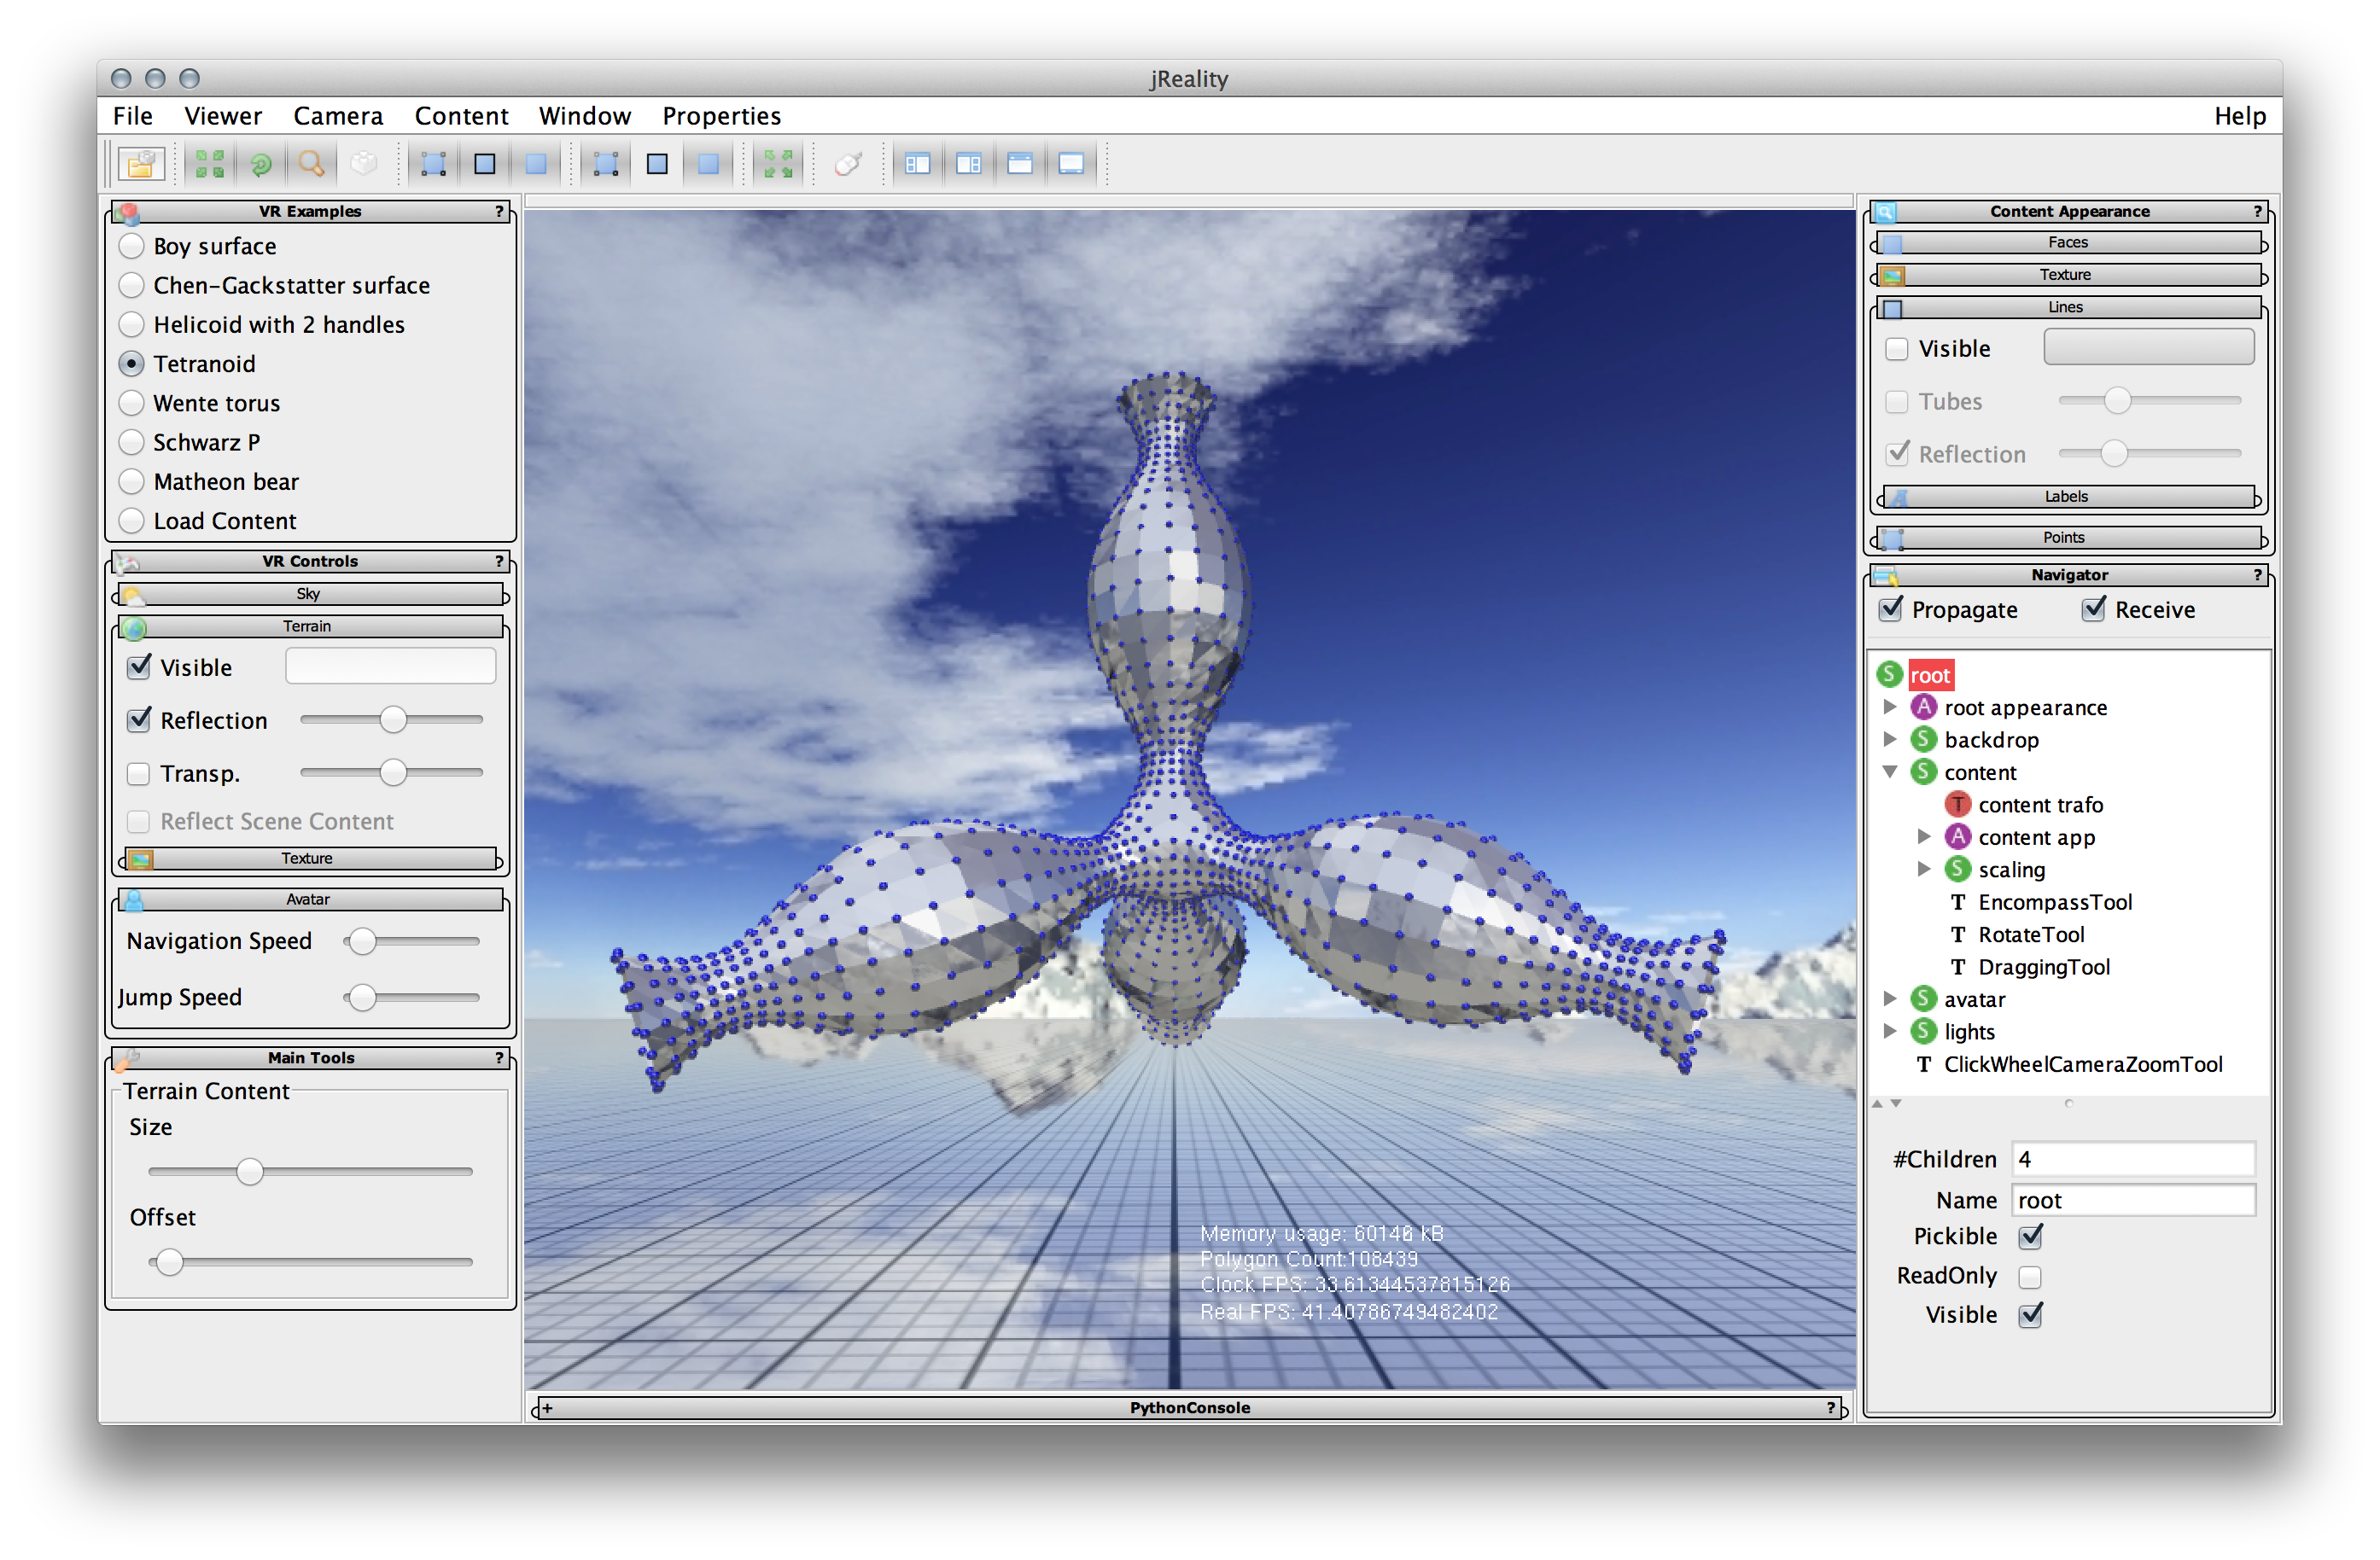
\includegraphics[width=9cm]{jrworkspace/jreality_hires.png}
\caption[The {\sc Jreality} user interface.]{The {\sc Jreality} user interface. A {\tt SideContainerPerspective} 
and {\tt ShrinkPanels} is used. The tool bar and 
menu bar is created by the aggregators described in Section~\ref{sec:reference_implementation}. This application
uses a set of predefined user interface features and virtual reality components. In a custom application the developer 
usually registeres only a subset of these featurs.}
\label{fig:jrworkspace_jreality}
\end{figure}

A custom {\sc Jreality} application is based on the {\tt JRViewer} class. This class uses {\tt SimpleController} to manage
plug-in registration and start-up. 

\subfilebibliography
\end{document}

%%% Local Variables:
%%% TeX-master: "Thesis.tex"
%%% End:
\documentclass[Thesis.tex]{subfiles}
\begin{document}

\chapter{The {\sc Jtem} libraries {\sc HalfEdge} and {\sc HalfEdgeTools}}
\label{chp:halfedge}

This chapter describes the {\sc Java} implementation of a half-edge data structure and a set of tools
combined in the package {\sc HalfEdgeTools}. Both packages are part of the {\sc Jtem} project
\cite{JtemWebsite}. This is joint work with Boris~Springborn ({\sc HalfEdge}), Thilo~R{\"o}rig, 
Felix~Kn{\"o}ppel, and Kristoffer Josefsson ({\sc HalfEdgeTools}), and
other contributers to the {\sc Jtem} project.

This implementation of a half-edge data structure was inspired by an implementation 
contained in the {\sc Cgal} library \cite{Kettner2000}.
This specific implementation is however different from existing libraries as is uses the generic
programming concept of {\sc Java} to achieve compatibility and flexibility.

The code presented in this section is compatible with {\sc Java} version 1.7 or later.

\label{sec:halfedge_halfedgetools}
\section{The {\sc HalfEdge} data structure}
\label{sec:halfedge}

Half-edge data structures are used primarily to represent cell decompositions of oriented surfaces.
We say "primarily" because half-edge data structures can be used to represent somewhat more general
combinatorial structures, such as, for example, a checker board surface with white squares removed.

Here, surface means two-dimensional manifold, possibly with boundary; and a cell decomposition 
of a surface is a graph embedded in the surface such that the complement of the graph is 
(topologically) a disjoint union of open disks. The term map on a surface means the same. 
Thus, a cell decomposition decomposes a surface into vertices, edges, and faces.

{\bf Regular and strongly regular}

A cell decomposition of a surface is called regular, if it has no loops (edges with the same vertex 
on both ends), and if the boundary of a face contains an edge or vertex at most once. It is called 
strongly regular if two edges have at most one vertex in common, and if two faces have at most 
one edge or one vertex in common. A strongly regular cell decomposition is usually called a mesh.

{\bf This half-edge data structure implementation}

This half-edge data structure implementation consists of different types of objects representing 
vertices, half-edges, and faces. The term half-edge can and should be thought of as synonymous
with oriented edge or directed edge.

Every half-edge object holds references to:

\begin{itemize}
\item its oppositely oriented companion edge
\item the next edge in the boundary of the face on its left hand side
\item the previous edge in the boundary of the face on its left hand side
\item the face on its left hand side
\item the vertex it points to.
\end{itemize}

The face and vertex objects hold back references to a half-edge referencing them. Finally, there 
is the class {\tt de.jtem.halfedge.HalfEdgeDataStructure} representing a whole half-edge data 
structure. It acts as a container for (and sort of factory of) its vertices, half-edges, and faces.

{\bf Use of Generics}

Typically, one wants to equip vertices, edges, and faces with additional properties or functionality. 
For example, vertices may have coordinates associated with them, edges may have weights, and 
faces may have colors.

Our half-edge data structure facilitates this by using generic classes as abstract base classes for 
vertex, edge, and face types: The classes {\tt de.jtem.halfedge.Vertex}, {\tt de.jtem.halfedge.Edge}, 
{\tt de.jtem.halfedge.Face} are all parameterized with the associated vertex, edge, and face types.

{\bf Example}

To create a half-edge data structure with vertices that have 2D coordinates, proceed as follows.

\begin{itemize}
\item{Step 1.} 
Define appropriate subclasses of {\tt de.jtem.half\-edge.Vertex}, {\tt de.jtem.half\-edge.Edge}, and 
{\tt de.jtem.halfedge.Face}, for example:

\begin{lstlisting}[numbers=none]
public class MyVertex extends Vertex<MyVertex, MyEdge, MyFace> {
	public Point2D p;
}
public class MyEdge extends Edge<MyVertex, MyEdge, MyFace> { }
public class MyFace extends Face<MyVertex, MyEdge, MyFace> { }
\end{lstlisting}

Of course you might make the property {\tt p} of {\tt MyEdge} private and provide getter and setter 
methods, etc. Note that you always have to subclass {\tt de.jtem.half\-edge.Vertex}, 
{\tt de.jtem.half\-edge.Edge}, and {\tt de.jtem.half\-edge.Face}, even if you do not define any 
additional functionality or properties.

\item{Step 2.} 
Instantiate a {\tt de.jtem.halfedge.HalfEdgeDataStructure}:

\begin{lstlisting}[numbers=none]
HalfEdgeDataStructure<MyVertex, MyEdge, MyFace> heds = new HalfEdgeDataStructure<>(MyVertex.class, MyEdge.class, MyFace.class);
\end{lstlisting}

The parameters of the constructor serve as run time type tokens. Alternatively you can create a subclass
of {\tt de.jtem.halfedge.HalfEdgeDataStructure} and create an instance of this:

\begin{lstlisting}[numbers=none]
public class MyHDS extends HalfEdgeDataStructure<MyVertex, MyEdge, MyFace> {
	public MyHDS() {
		super(MyVertex.class, MyEdge.class, MyFace.class);
	}
}
...
MyHDS mds = new MyHDS();
\end{lstlisting}

\item{Step 3.} 
Instantiate vertices, edges, and faces using the {\tt addNewVertex}, {\tt addNewEdge}, and 
{\tt addNewFace} methods, like this:

\begin{lstlisting}[numbers=none]
MyVertex v = heds.addNewVertex();
MyEdge e = heds.addNewEdge();
MyFace f = heds.addNewFace();
\end{lstlisting}

\end{itemize}

{\bf Linkage and incidence.}

Node classes provide methods to create a valid data structure. Most of the methods are bidirectional linkage methods that affect the target and the caller. The corresponding methods are:
\begin{itemize}
\item {\tt E.linkNextEdge} sets the {\tt nextEdge} property of this edge as well as the 
{\tt previousEdge} property of the given edge.
\item {\tt E.linkOppositeEdge} sets the {\tt oppositeEdge} property of this edge and of the given edge accordingly.
\item {\tt E.linkPreviousEdge} sets {\tt previousEdge} and {\tt nextEdge} properties of this and the given edge.
\item {\tt E.setLeftFace} sets the {\tt leftFace} property of this edge and the {\tt boundaryEdge} property of the given face.
\item {\tt E.setTargetVertex} sets the {\tt targetVertex} property of this edge and the 
{\tt incommingEdge} property of the given vertex.
\end{itemize}

{\bf Node indices.}

During algorithm development it is often necessary to access consistent indices on vertices,
half-edges, or faces. We support this operation by the {\tt index} field of nodes accessible via
the {\tt getIndex()} method of all node types. Nodes are required to have indices $0,\ldots,\#V$,
$0,\ldots,\#E$, and $0,\ldots,\#F$ respectively. Note that $\#E$ is the number of half-edges
in the data structure. The running time of a {\tt getIndex} operation is $\mathcal{O}(1)$ if
no {\tt remove} operation has invalidated the indices. Otherwise it is $\mathcal{O}(n)$ where
$n$ is the number of nodes in the data structure, e.g., $n=\#V$.

{\bf Iterating and directly accessing nodes.}

Nodes can be directly accessed via the corresponding {\tt get} method. It takes the node index
and returns the node with the given index. It is guaranteed that for a given $i\in \{0,\ldots,\#N\}$
it is {\tt getNode($i$).getIndex()$ = i$}.
Nodes in the data structure can be iterated over using one of the methods {\tt getVertices}, 
{\tt getEdges}, or {\tt getFaces}. These return unmodifiable instances of {\tt java.util.List} containing the respective node instances.

{\bf Undirected edges}

A half-edge has the {\tt positive} property. In a pair of opposite edges it is required that the boolean
value of this property is different, i.e., \url{e.isPositive()} $!=$ \url{e.getOppositeEdge().isPositive()}.
Using this property it is possible to iterate over undirected edges, i.e., the positive or the negative
half-edges. The methods {\tt getPositiveEdges} and {\tt getNegativeEdge} of the data structure 
implement this.

{\bf Removing nodes from a data structure.}

A node can be deleted from the data structure using the {\tt removeVertex/Edge/Face} methods.
The running time of a remove operation is always $\mathcal{O}(1)$. Node indices however will
get invalidated and reindexed on the next access of any index related operation that in turn will
then have running time $\mathcal{O}(n)$.

{\bf Half-Edge utilities.}

To work efficiently with half-edge data a set of algorithms is implemented as static utility methods
in the class {\tt de.jtem.half\-edge.util.Half\-Edge\-Utils}. It contains methods that help iterating 
over incoming edges at a vertex, or iterating over the boundary edges of a surface or a face, and many more.


\section{Data, Algorithms, and Tools}

A set of algorithms and tools is implemented in the {\sc Jtem} project {\sc HalfEdgeTools}
\cite{JtemWebsite}. 

Many algorithms in the library are purely combinatorial. This means there is no extra data 
involved during algorithm execution. Thus such an algorithm is generic by definition. The
method signature could look like this:

\begin{lstlisting}
public static <
	V extends Vertex<V, E, F>,
	E extends Edge<V, E, F>,
	F extends Face<V, E, F>,
	HDS extends HalfEdgeDataStructure<V, E, F>
> void triangulate(HDS hds){
	...
}
\end{lstlisting}

This method works on any half-edge data structure that is either an instance of {\tt
de.jtem.half\-edge.HalfEdgeDataStructure} or an instance of a sub-class. This method
signature makes the algorithm code itself look very clean. For instance iterating over
all vertices amounts to:

\begin{lstlisting}
for (V v : hds.getVertices()) {
	E e = v.getIncomingEdge();
	...
}
\end{lstlisting}

On the other hand when designing a generic algorithm that needs certain data associated
with nodes we have basically two options. Option 1. requires the generic node classes to
implement the required interfaces:

\begin{lstlisting}
public static <
	V extends Vertex<V, E, F> & HasCoordinate3D,
	E extends Edge<V, E, F>,
	F extends Face<V, E, F>,
	HDS extends HalfEdgeDataStructure<V, E, F>
> void convexHull(HDS hds){
	...
	Coordinate3D x = v.getCoordinate3D();
}
\end{lstlisting}

This forces the Vertex implementations that use this algorithm to implement an interface
called {\tt HasCoordinate3D}. It leads to explicit and clean code of the algorithm. A drawback of this
is that an existing implementation that should use this algorithm has to be adapted to implement the 
possibly many interfaces required by the algorithm. 
This is not a feasible solution when is comes to a modular application where algorithms come as 
plug-ins without the chance to change the data structure.

{\bf AdapterSet and Adapters}

The second option uses the concept of adapters and is implemented in the package {\tt
de.jtem.\-halfedge\-tools.adapter}. An adapter defines a map from nodes to a data type supported 
by the adapter. We first show how this concept works when designing algorithms and then
describe the implementation of the required adapters. 

In this next example we calculate the discrete Dirichlet energy of a double valued function with 
double valued weights on edges. 

\lstinputlisting[
	caption={Algorithm that uses data from the {\tt AdapterSet}. The {\tt get} method of the
		{\tt AdapterSet} takes the data class type to find a matching adapter (Line~12 and 13).
		The corresponding {\tt getDefault} method takes a default value that is returned if no
		matching adapter is found (Line~14). It uses {\tt @FunctionValue} and {\tt @Weight} annotated 
		adapters to acquire the data needed for calculation of the output value.
	},
	label=alg:dirichlet,
	captionpos=b,
	firstline=14,
	lastline=31
]{java/de/sechel/thesis/MyUtility.java}

This method requires the {\tt AdapterSet} to contain adapters that provide
{\tt @FunctionValue} data on vertices (Line~12 and 13) and {\tt @Weight} data on half-edges (Line 14). 

The classes {\tt FunctionValue} and {\tt Weight} are runtime annotation classes, e.g.,

\begin{lstlisting}
@Retention(RetentionPolicy.RUNTIME)
@Target(ElementType.TYPE)
public @interface FunctionValue {}
\end{lstlisting}

An adapter class annotated with this annotation serves as {\tt @FunctionaValue} data adapter when 
called for as in Line 11-13 of Listing~\ref{alg:dirichlet}. The meaning of adapter annotations is 
an agreement between the algorithm using it and the implementor of the adapter. It is subject
of a best-practice policy to implement the adapters such that they output data that fit its 
annotation names.

There are three basic classes that could serve as base class of an adapter. It is

\begin{itemize}
\item {\tt Adapter} - The abstract base class of all adapters. Should never be subclassed directly.
\item {\tt AbstractAdapter} - A adapter class that knows about the supported data type and implements
all getter and setter methods. Here only the needed methods can be overwritten. Node type checking
is done manually thus allows for the creation of generic adapters.
\item {\tt AbstractTypedAdpter} - If you know which half edge node classes the adapter is supposed to
work with this is the adapter base class you should use. Node type checking and casting is done in the
super class.
\end{itemize}

An adapter implementation using the {\tt AbstractAdapter} is for instance:

\lstinputlisting[
	caption={
		Adapter implementation using the {\tt AbstractAdapter} as base class and a 
		map as storage concept for double values on generic vertices. It is annotated 
		with a {\tt @FunctionValue} annotation to serve as
		provider for data in the {\tt AdapterSet} (Line 1). The super class {\tt
		AbstractAdapter} is parameterized with the data type of the implementation; In this
		case {\tt Double} (Line 2). 
		The super class constructor is invoked with the class object of this type and flags 
		that tell the adapter
		if get and/or set operations are permitted (Line 6). The method {\tt canAccept}
		decides whether the adapter can work with the given node class; In this case the 
		adapter can accept any {\tt Vertex} object (Line 12). 
		Vertex getter and setter methods are generic methods (Line 16 to 32). 
	},
	label=lst:adapter,
	captionpos=b,
	firstline=13,
	lastline=50
] {java/de/sechel/thesis/MyAbstractAdapter.java}

When writing the adapter for concrete node classes we have a more concise description:

\lstinputlisting[
	caption={
		An adapter using {\tt AbstractTypedAdpter} as base class. Also annotated with the {\tt
		@FunctionValue} annotation. This super class is parameterized
		with a set of node class implementations and the adapter data type. Here the super
		constructor takes the node class objects or {\tt null} if a node type is not supported, the
		data type class object, and the getter/setter flags. The vertex getter and setter methods 
		are not generic and the corresponding casting is done in the super class. Adapters working
		on edges or faces implement the corresponding {\tt get/setEdgeValue} or 
		{\tt get/setFaceValue} methods.
	},
	label=lst:adapter_typed,
	captionpos=b,
	firstline=9,
	lastline=50
] {java/de/sechel/thesis/MyTypedAdapter.java}

Using this concept of typed adapters the usage of an algorithm amounts to the implementation of
required data adapters and the creation of a suitable {\tt AdapterSet}.

\lstinputlisting[
	caption={Usage example of the algorithm presented in Listing~\ref{alg:dirichlet}. In this example 
	an empty data structure is created, filled with a dodecahedron combinatorics, and then processed by the 	
	algorithm. The {\tt AdapterSet} contains the {\tt @FunctionValue} annotated adapter to provide 
	{\tt Double} values on vertices. In this example a {\tt @Weight} adapter in not needed since the 
	{\tt computeDirichlet} algorithm uses the {\tt getDefault} method to obtain weight data for edges.},
	label=alg:dirichlet_usage,
	captionpos=b,
	firstline=33,
	lastline=40
]{java/de/sechel/thesis/MyUtility.java}

{\bf Generic Adapters}

There is a set of generic adapters implemented in the package 
{\tt de.jtem.half\-edge\-tools.adap\-ter.generic}. Here generic means that the adapter does not provide
the data itself. Instead it asks for other adapters to provide data and converts, merges, or recalculates its
output based on the data acquired from other adapter implementations.

The most important example of pre-defined generic adapters are position and texture position adapters.
These adapters come in three versions, e.g., {\tt @Position2D}, {\tt @Position3D}, and {\tt @Position4D}. The implementations, e.g, {\tt de.jtem.half\-edge\-tools.adapter.generic.Position\-3dAdapter} obtain position
data from the {\tt AdapterSet} using the adapter annotated with {\tt @Position} and convert if the lengths
of arrays is not equal to $3$.

An algorithm using generic adapters is free of data conversion code.


{\bf Error Handling}

If a data adapter that is used by an algorithm is not found, the {\tt AdapterSet} throws exceptions stating
the name of the required annotation and the node type that is expected. 

\begin{lstlisting}[
numbers=none, stringstyle=\ttfamily,keywordstyle=\ttfamily, numbersep=0pt,xleftmargin=20pt
]
Exception in thread "main" de.jtem.halfedgetools.adapter.AdapterException: Adapter "FunctionValue" for node VV not found
	at de.jtem.halfedgetools.adapter.AdapterSet.get(Unknown Source)
	at de.sechel.thesis.MyUtility.computeDirichlet(MyUtility.java:25)
	at de.sechel.thesis.MyUtility.calculate(MyUtility.java:39)
	at de.sechel.thesis.MyUtility.main(MyUtility.java:44)
\end{lstlisting}


\section{{\sc HalfEdgeTools} and {\sc Jreality}}
\label{sec:halfedge_tools_visualization}

The {\sc HalfEdgeTools} package contains utility classes for the visualization of half-edge data with 
{\sc Jreality} \cite{JrealityWebsite}. It is part of the {\sc Jtem} project \cite{JtemWebsite}. 

{\bf Half-edge Interface}

A central role plays the plug-in {\tt de.jtem.halfedge\-tools.plugin.Halfedge\-Interface}. This plug-in works 
as a converter between half-edge data structure and {\tt IndexedFaceSet} data structure used internally 
by {\sc Jreality}. It creates a user interface that contains GUI elements for layer management, import, export,
undo, redo, and more features, see Figure~\ref{fig:halfedge_interface}.

\begin{figure}
	\centering
	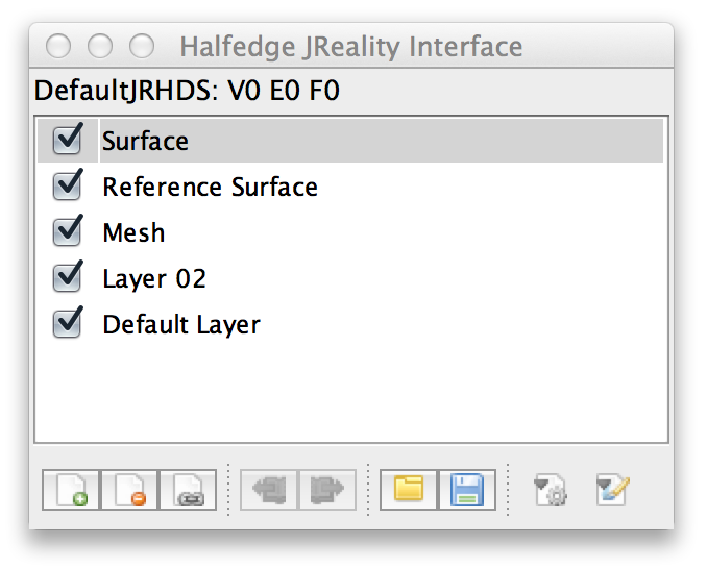
\includegraphics[width=5cm]{jrworkspace/halfedge_interface_hires.pdf}
	\caption{The user interface created by the {\tt HalfedgeInterface} plug-in. It manages layers that
		contain different instances of half-edge data structures and the corresponding visualizations.
		Layers can be merged, {\tt OBJ} files can be exported and imported and visualization
		options can be adjusted. 
	}
	\label{fig:halfedge_interface}
\end{figure}

The API of the {\tt HalfedgeInterface} supports {\tt set} and {\tt get} methods that convert to and from
{\sc Jreality}. During conversion data is read from an {\tt AdapterSet} that is managed by the half-edge
interface. The plug-in supports various data on node types. We give a list of annotation types and
their purposes. All conversion adapters work with {\tt double[]} or {\tt double} data types. All
supported annotation types are in the package {\tt de.jtem.halfedgetools.adapter.type}.

\begin{itemize}
\item {\tt\bf @Position} - Positions of vertices can have lengths 2, 3, or 4.
\item {\tt\bf @Color} - Colors either on vertices, edges, or faces.
\item {\tt\bf @Normal} - Normals usually for vertices or faces.
\item {\tt\bf @TexturePosition} - Texture coordinates of length 2, 3, or 4.
\item {\tt\bf @Label} - Text annotations that appear next to the node.
\item {\tt\bf @Radius} - Radii of vertex sphere representations or edge cylinders when rendered
as spheres or tubes.
\item {\tt\bf @Size} - Size in pixels of vertex points or edge lines when rendered as points or lines.
\end{itemize}

Internally the conversion is done using the classes from the package 
{\tt de.jtem.halfedge\-tools.jreality}. Conversion from and to a {\sc Jreality} {\tt IndexedFaceSet}
is implemented in {\tt ConverterHeds2JR} and {\tt ConverterJR2Heds}.

{\bf Visualization Interface}

A second important plug-in is the {\tt Visuali\-zation\-Inter\-face}. It defines
an plug-in API and various implementations for data visualization with the half-edge data structure. 


\begin{figure}
	\centering
	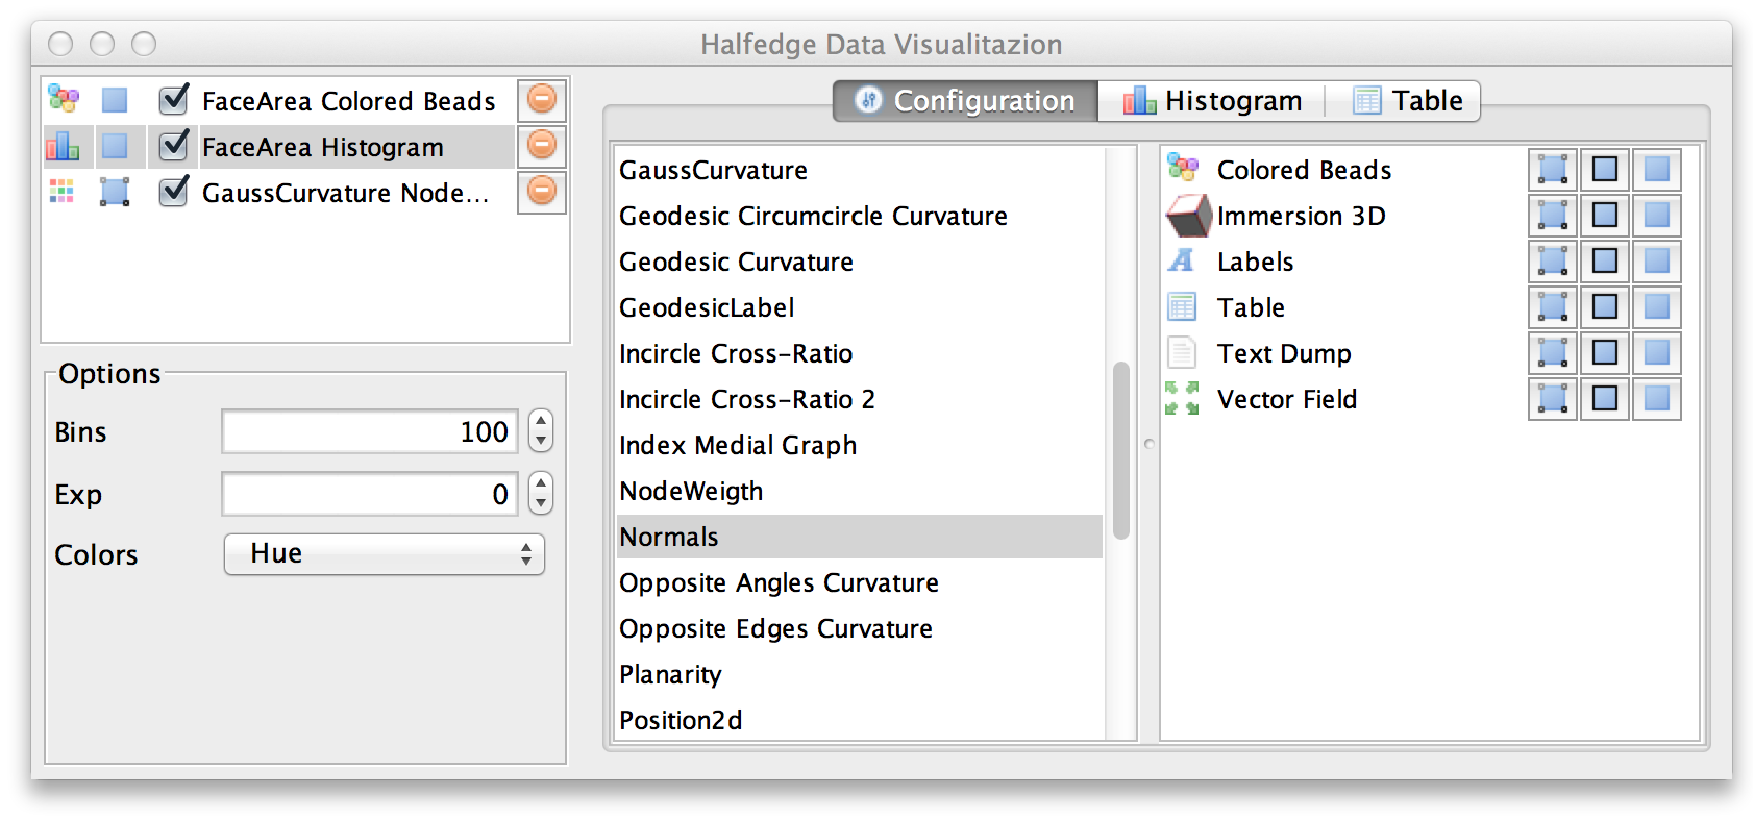
\includegraphics[width=11cm]{jrworkspace/visualization_interface_hires02.pdf}
	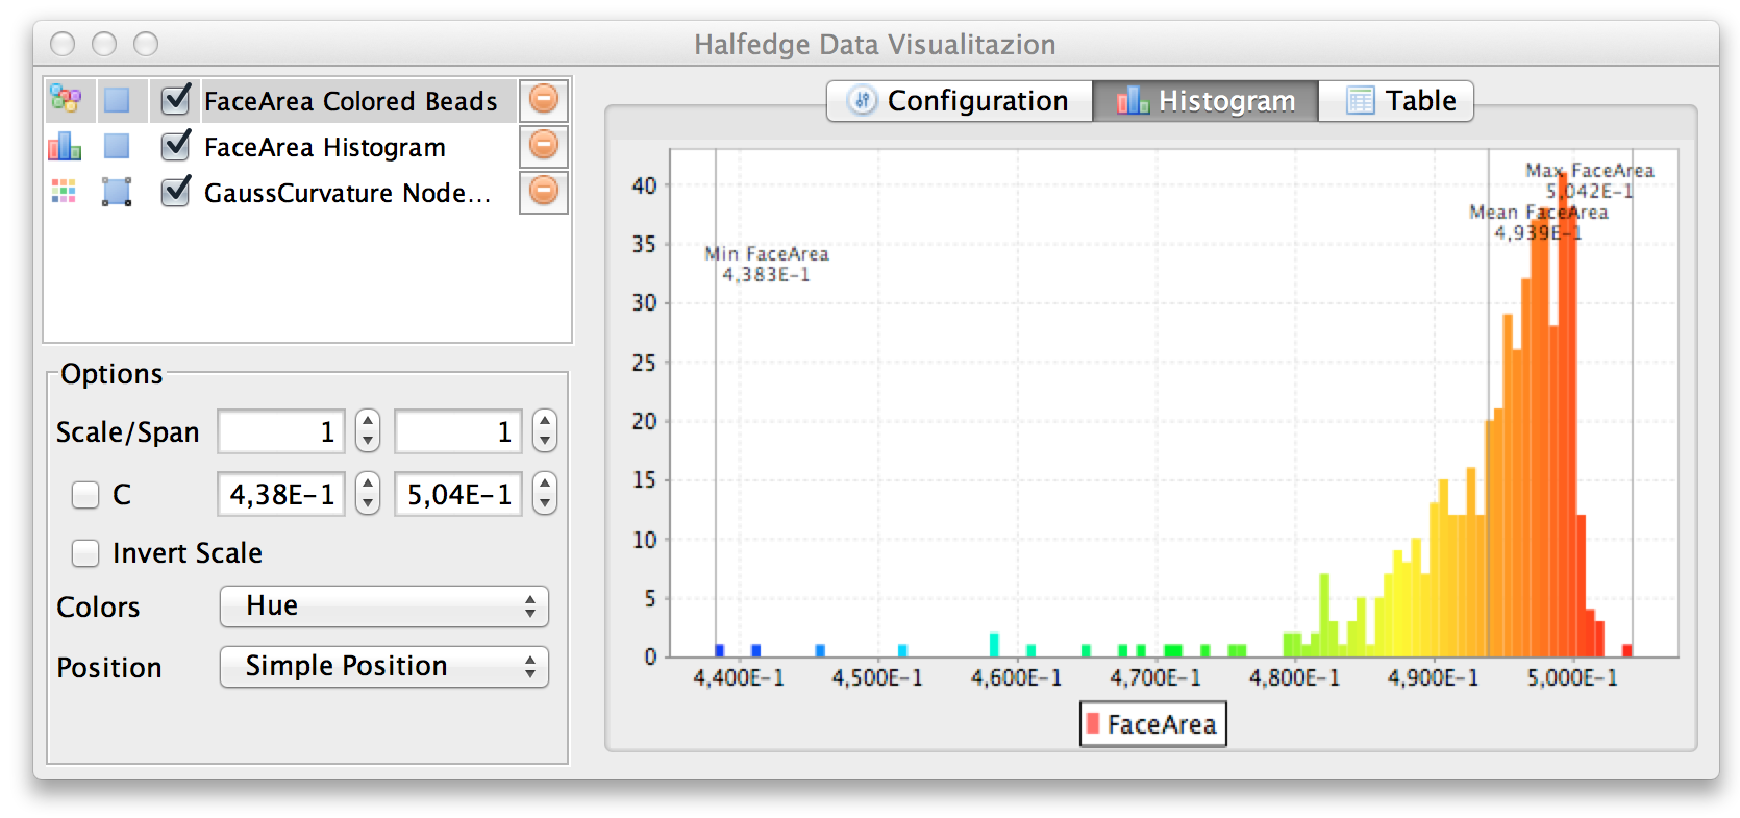
\includegraphics[width=11cm]{jrworkspace/visualization_interface_hires.pdf}
	\caption[Visualization Interface]{The half-edge visualization user interface. Selection of a visualization
		plug-in for a data adapter (top). A histogram view for scalar data on half-edge nodes (bottom).}
	\label{fig:visualization_interface}
\end{figure}

Every {\tt Adapter} that is managed by the {\tt HalfedgeInterface} is available as data source. In 
addition to this every plug-in extending {\tt de.jtem.half\-edgetools.plugin.data.Data\-Source\-Provider} 
is asked for data adapters. A list of these data sources is displayed in the user interface, see 
Figure~\ref{fig:visualization_interface} (top). A visualization of the selected data source is created by a
corresponding {\tt DataVisualizer} plug-in. For scalar data on vertices, edges, or faces we provide the 
colored beads visualizer or simply colored nodes, Figure~\ref{fig:visualizers}. There is a histogram that displays a density
plot for scalar data on nodes, Figure~\ref{fig:visualizers} (right) and Figure~\ref{fig:visualization_interface} (bottom). For vector valued data 
there is a visualizer that creates arrows starting at half-edge nodes.


\begin{figure}
	\centering
	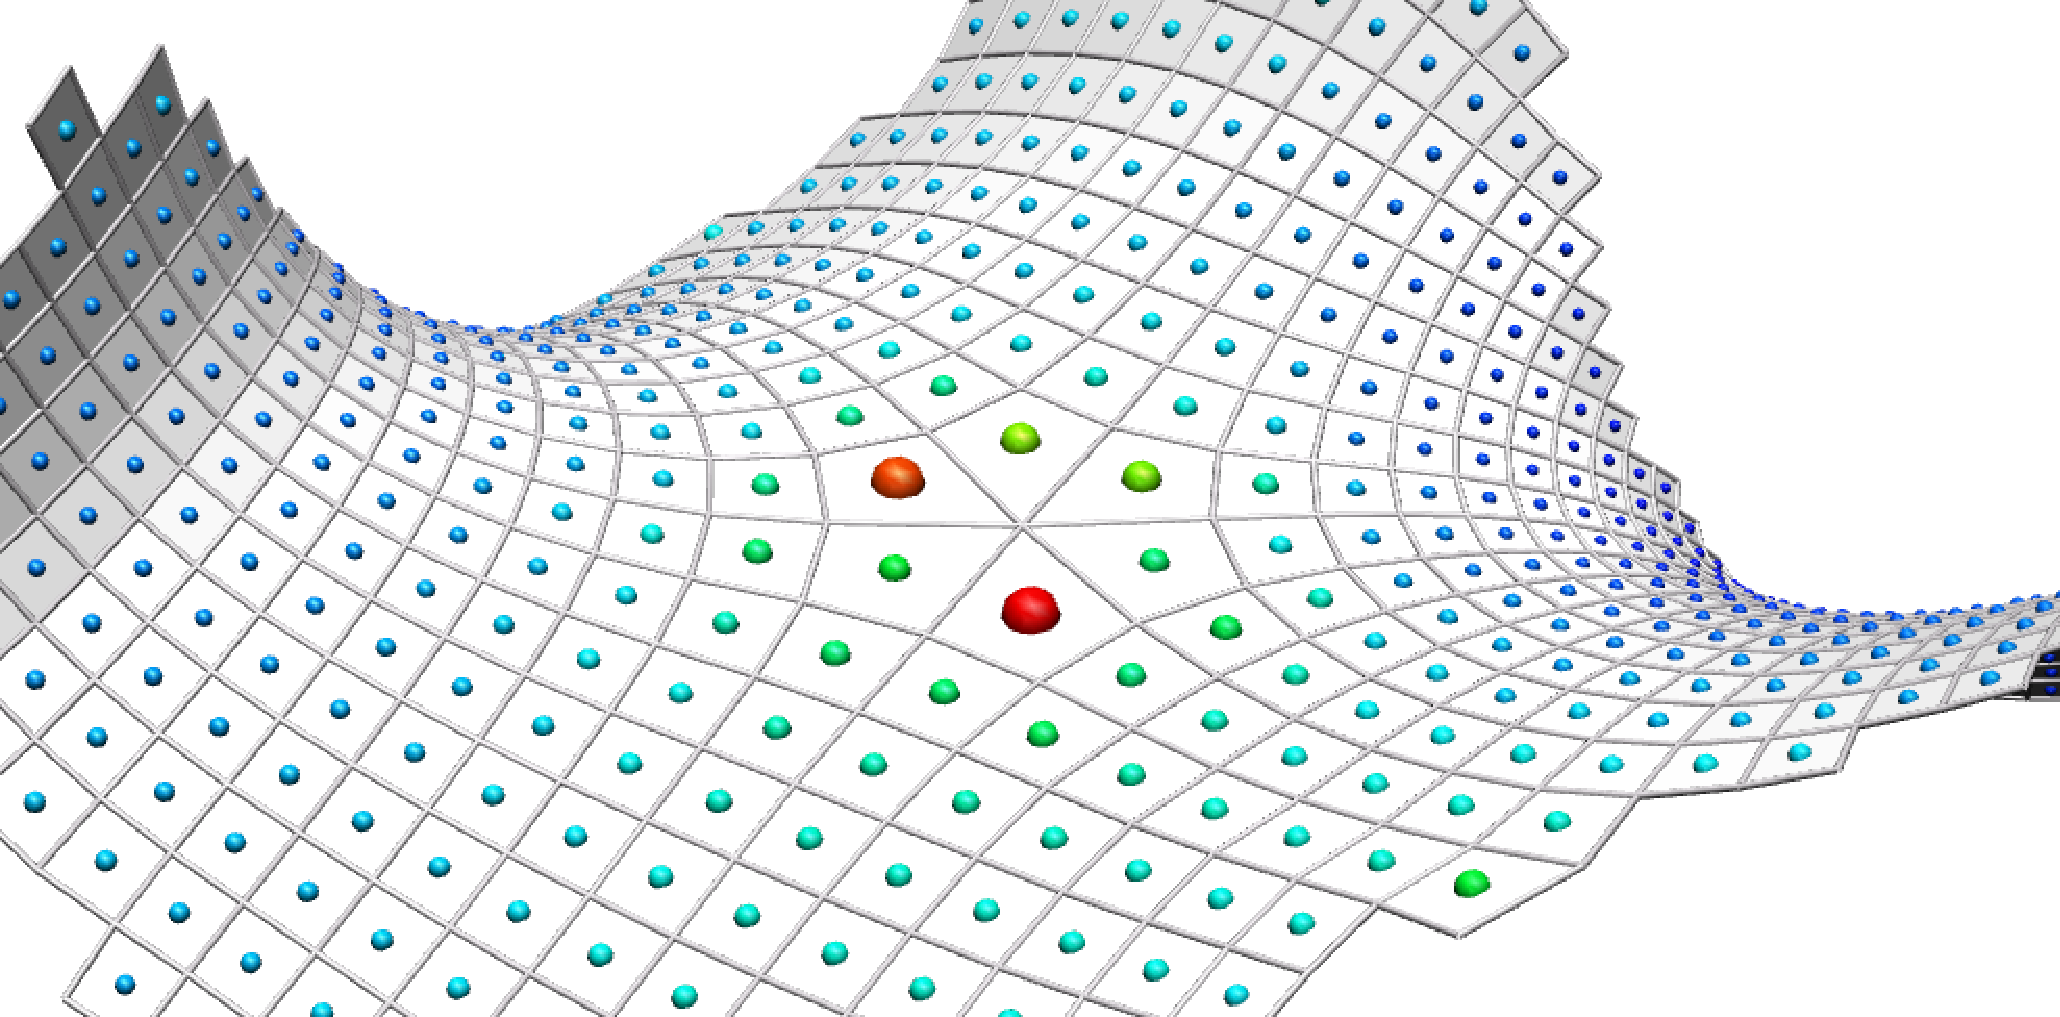
\includegraphics[width=4.5cm]{jrworkspace/colored_beads.pdf}
	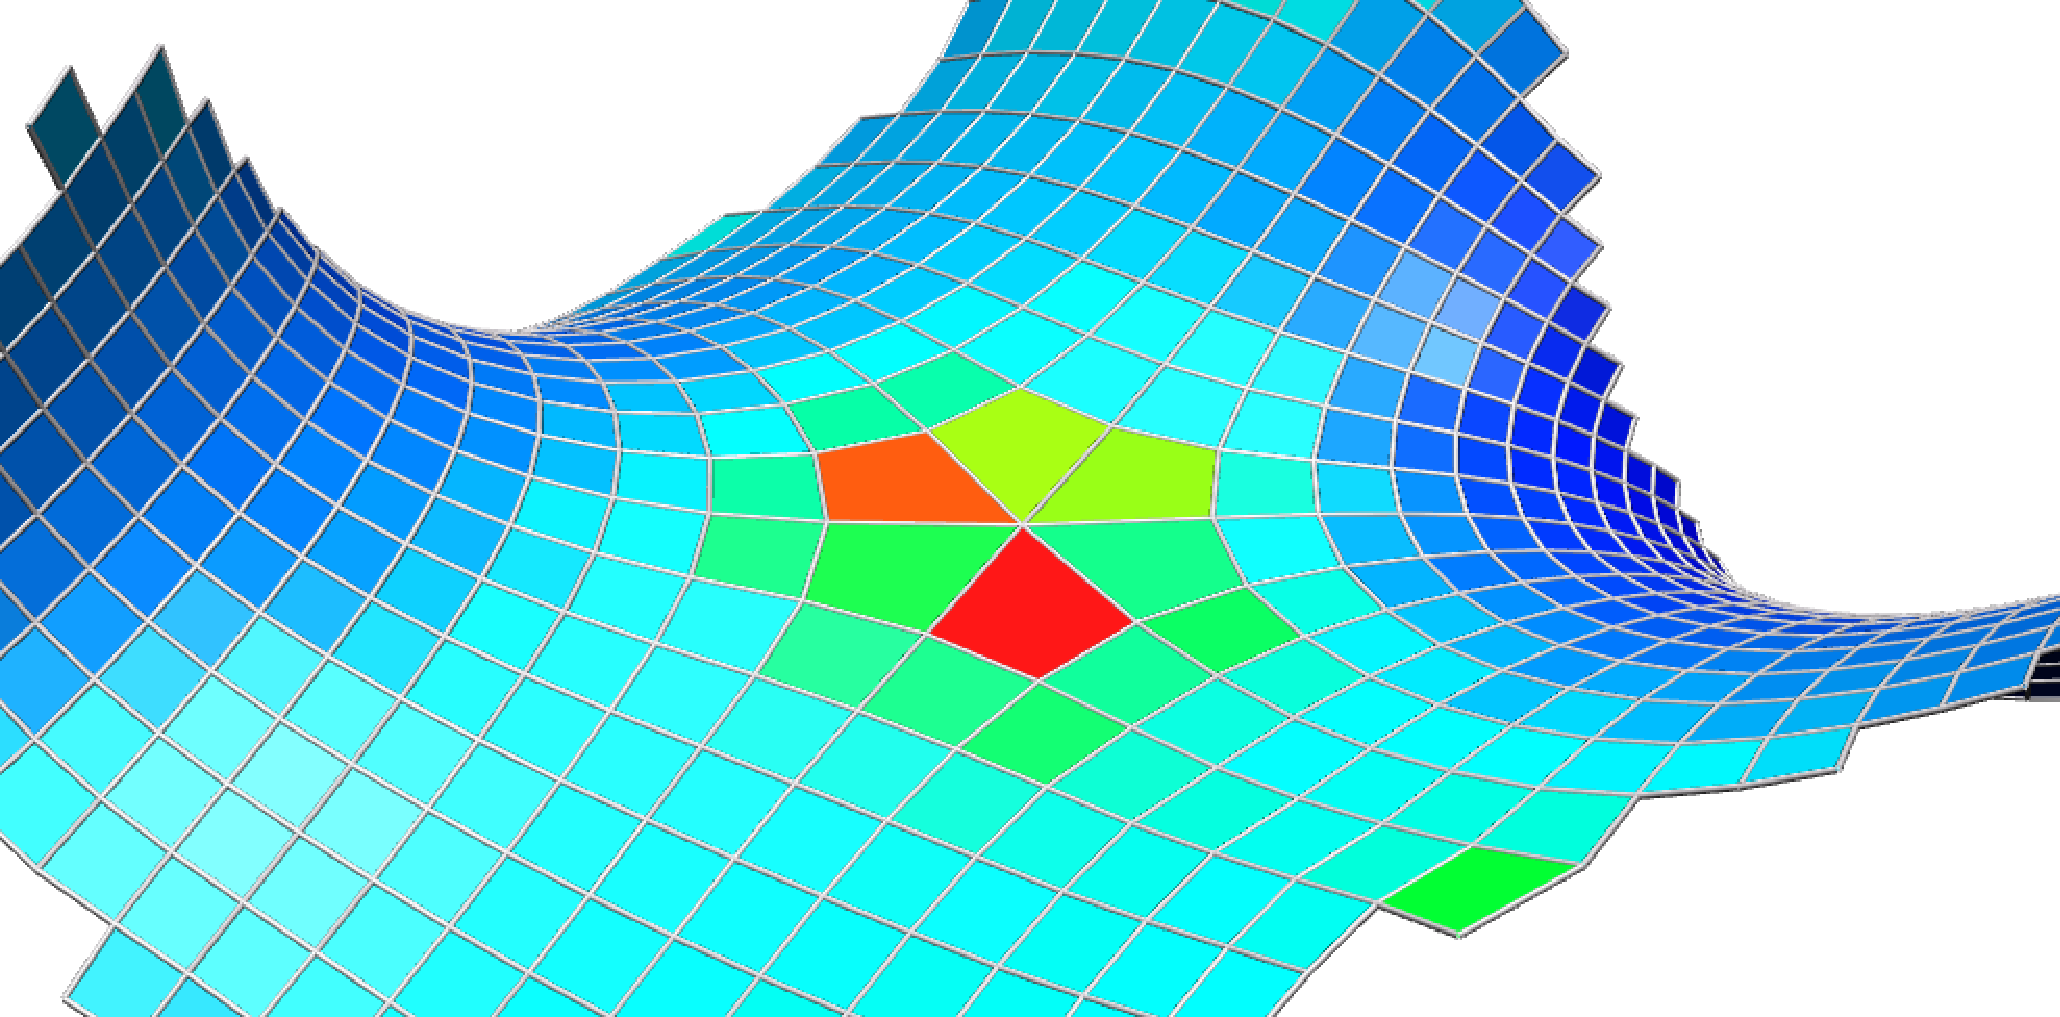
\includegraphics[width=4.5cm]{jrworkspace/node_colors.pdf}
	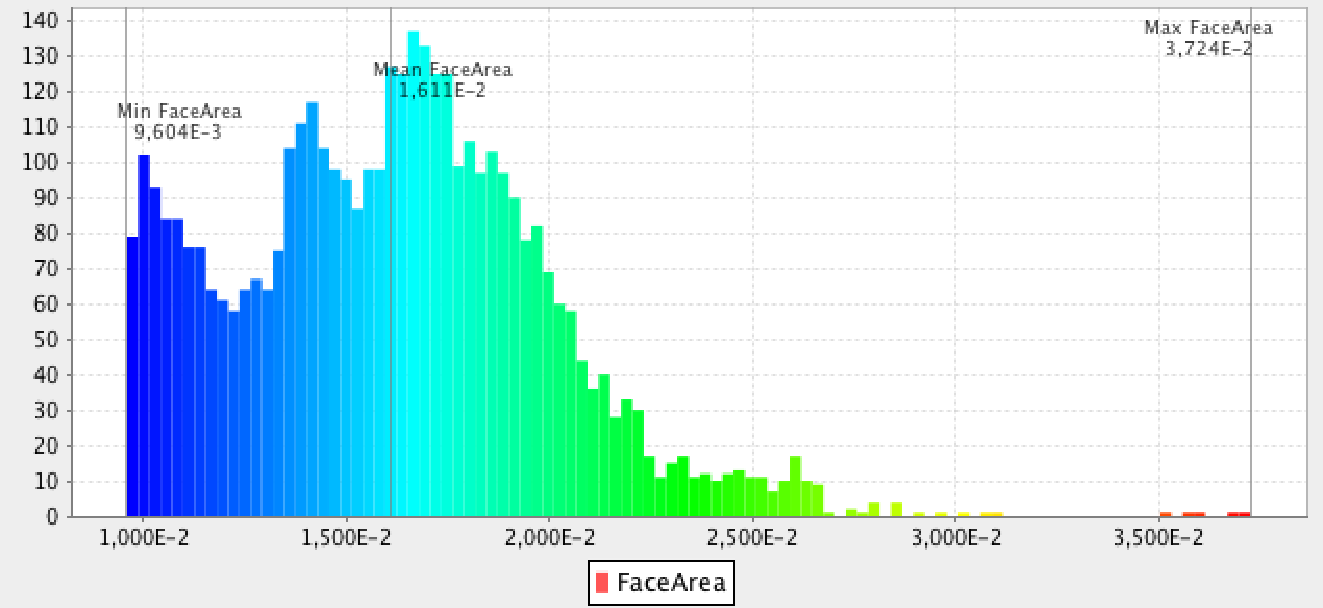
\includegraphics[width=5cm]{jrworkspace/histogram.pdf}
	\caption[Visualizers]{Different visualization plug-ins for scalar data on faces. Colored beads (left),
		node colors, and histogram view.}
	\label{fig:visualizers}
\end{figure}

\subfilebibliography
\end{document}

%%% Local Variables:
%%% TeX-master: "Thesis.tex"
%%% End:
\documentclass[Thesis.tex]{subfiles}
\begin{document}

\chapter{{\sc ConformalLab} - Conformal maps and uniformization}
\label{chp:conformallab}

\section{Data format}
\label{sec:conformal_data}
To store and process data {\sc ConformalLab} uses an {\sc XML} data format.
All examples presented in Chapter~\ref{chp:conformal_examples} are stored
in this format. 
All XML data is contained in the XML namespace 
{\tt http://www.varylab.com/conformallab/types}.


{\bf Schottky data} 

A Riemann surface can be given by Schottky data, see Section~\ref{sec:schottky_examples}. An example is shown in Listing~\ref{lst:schottky_xml}. {\tt SchottkyData} can include one or more {\tt SchottkyGenerator}s. A {\tt SchottkyGenerator} defines fix points $A$ and $B$, the complex number $\mu$, and a {\tt Circle}. This circle is required to contain $A$ and must not contain $B$.

\begin{lstlisting}[label=lst:schottky_xml, caption={A torus given by schotty data}, numbers=none, language=XML, captionpos=b]
<SchottkyData name="Schottky">
	<SchottkyGenerator>
		<A re="-1.0" im="0.0"/>
		<B re="1.0" im="0.0"/>
		<Mu re="0.25" im="0.0"/>
		<Circle radius="1.3">
			<Center re="-1.6" im="0.0"/>
		</Circle>
	</SchottkyGenerator>
</SchottkyData>
\end{lstlisting}

{\bf Hyperelliptic data} 

Hyperelliptic algebraic curves as used in the examples of Section~\ref{sec:examples_elliptic} and \ref{sec:examples_hyperelliptic} are given by the location of their branch points in the complex plane.

\begin{lstlisting}[label=lst:hyperelliptic_xml, caption={A torus given as hyperelliptic data}, numbers=none, language=XML, captionpos=b]
<HyperEllipticAlgebraicCurve name="Curve g2">
	<BranchPoint re="-0.5" im="-1.0"/>
	<BranchPoint re="0.5" im="-1.0"/>
	<BranchPoint re="1.0" im="0.0"/>
	<BranchPoint re="-1.0" im="0.0"/>
</HyperEllipticAlgebraicCurve>
\end{lstlisting}

\begin{lstlisting}[label=lst:hyperelliptic_xml, caption={A torus given as {\tt HalfedegeEmbedding}
with identified edge pairs and vertices.}, numbers=none, language=XML, captionpos=b]
<HalfedgeEmbedding name="Uniformizing Map_domain">
	<Vertex x="0.0" y="0.0" z="0.0" w="1.0" index="0"/>
	<Vertex x="1.0" y="0.0" z="0.0" w="1.0" index="1"/>
	<Vertex x="1.0" y="1.0" z="0.0" w="1.0" index="2"/>
	<Vertex x="0.0" y="1.0" z="0.0" w="1.0" index="3"/>
	<Identification>
		<Vertex>0</Vertex>
		<Vertex>1</Vertex>
		<Vertex>2</Vertex>
		<Vertex>3</Vertex>
	</Identification>
	<Halfedge left="0" target="1" next="1" opposite="4" index="0"/>
	<Halfedge left="0" target="2" next="2" opposite="5" index="1"/>
	<Halfedge left="0" target="3" next="3" opposite="6" index="2"/>
	<Halfedge left="0" target="0" next="0" opposite="7" index="3"/>
	<Halfedge left="-1" target="0" next="7" opposite="0" index="4"/>
	<Halfedge left="-1" target="1" next="4" opposite="1" index="5"/>
	<Halfedge left="-1" target="2" next="5" opposite="2" index="6"/>
	<Halfedge left="-1" target="3" next="6" opposite="3" index="7"/>
	<EdgeIdentification edge1="0" edge2="4" edge3="2" edge4="6"/>
	<EdgeIdentification edge1="1" edge2="5" edge3="3" edge4="7"/>
	<Face index="0"/>
</HalfedgeEmbedding>
\end{lstlisting}

\begin{lstlisting}[label=lst:hyperelliptic_xml, caption={A discrete map is given by a pair of embeddings, the {\tt Domain} and {\tt Image} of the map. Both are of type {\tt HalfedgeEmbedding}.}, numbers=none, language=XML, captionpos=b]
<HalfedgeMap name="Uniformizing Map">
	<Domain name="Uniformizing Map_domain">
		...
	</Domain>
	<Image name="Uniformizing Map_image">
		...
	</Image>
</HalfedgeMap>
\end{lstlisting}

\begin{lstlisting}[label=lst:hyperelliptic_xml, caption={A torus given by its uniformizing group and a fundamental polygon. The elements of the group are either euclidean motions or hyperbolic motions given as elements of $\mathbb PSL_2$.}, numbers=none, language=XML, captionpos=b]
<UniformizationData name="Direct Uniformization">
	<UniformizingGroup>
		<IsometryPSL2R 
			m11="1.0" m12="0.0" m13="1.0" 
			m21="0.0" m22="1.0" m23="0.0" 
			m31="0.0" m32="0.0" m33="1.0"
		/>
		<IsometryPSL2R 
			m11="1.0" m12="0.0" m13="0.0" 
			m21="0.0" m22="1.0" m23="1.0" 
			m31="0.0" m32="0.0" m33="1.0"
		/>
		<IsometryPSL2R 
			m11="1.0" m12="0.0" m13="-1.0" 
			m21="0.0" m22="1.0" m23="0.0" 
			m31="0.0" m32="0.0" m33="1.0"
		/>
		<IsometryPSL2R 
			m11="1.0" m12="0.0" m13="0.0" 
			m21="0.0" m22="1.0" m23="-1.0" 
			m31="0.0" m32="0.0" m33="1.0"
		/>
	</UniformizingGroup>
	<FundamentalPolygon>
		<FundamentalVertex index="0"/>
		<FundamentalEdge index="0" nextEdge="1" previousEdge="3" identifiedEdge="2" startVertex="0">
			<StartPosition re="0.0" im="0.0"/>
		</FundamentalEdge>
		<FundamentalEdge index="1" nextEdge="2" previousEdge="0" identifiedEdge="3" startVertex="0">
			<StartPosition re="1.0" im="0.0"/>
		</FundamentalEdge>
		<FundamentalEdge index="2" nextEdge="3" previousEdge="1" identifiedEdge="0" startVertex="0">
			<StartPosition re="1.0" im="1.0"/>
		</FundamentalEdge>
		<FundamentalEdge index="3" nextEdge="0" previousEdge="2" identifiedEdge="1" startVertex="0">
			<StartPosition re="0.0" im="1.0"/>
		</FundamentalEdge>
	</FundamentalPolygon>
</UniformizationData>
\end{lstlisting}

\begin{lstlisting}[label=lst:hyperelliptic_xml, caption={A wente torus given by a discrete metric. Vertices are given implitly
by following the order of triangle glueings.}, numbers=none, language=XML, captionpos=b]
<DiscreteMetric name="Torus Discrete Metric">
	<MetricEdge length="1.0" index="0"/>
	<MetricEdge length="1.0" index="1"/>
	<MetricEdge length="1.0" index="2"/>
	<MetricEdge length="1.0" index="3"/>
	<MetricEdge length="1.0" index="4"/>
	<MetricEdge length="1.0" index="5"/>
	<MetricEdge length="1.0" index="6"/>
	<MetricEdge length="1.0" index="7"/>
	<MetricEdge length="1.0" index="8"/>
	<MetricEdge length="1.0" index="9"/>
	<MetricEdge length="1.0" index="10"/>
	<MetricEdge length="1.0" index="11"/>
	<MetricTriangle edge1="2" edge2="6" edge3="1"/>
	<MetricTriangle edge1="4" edge2="0" edge3="3"/>
	<MetricTriangle edge1="2" edge2="11" edge3="3"/>
	<MetricTriangle edge1="4" edge2="5" edge3="1"/>
	<MetricTriangle edge1="0" edge2="7" edge3="8"/>
	<MetricTriangle edge1="6" edge2="9" edge3="10"/>
	<MetricTriangle edge1="9" edge2="8" edge3="5"/>
	<MetricTriangle edge1="7" edge2="10" edge3="11"/>
</DiscreteMetric>
\end{lstlisting}


\section{User interface}

The user interface of {\sc ConformalLab} is devided into panels which serve
separate purposes.
\begin{wrapfigure}{R}{0.4\textwidth}
\centering
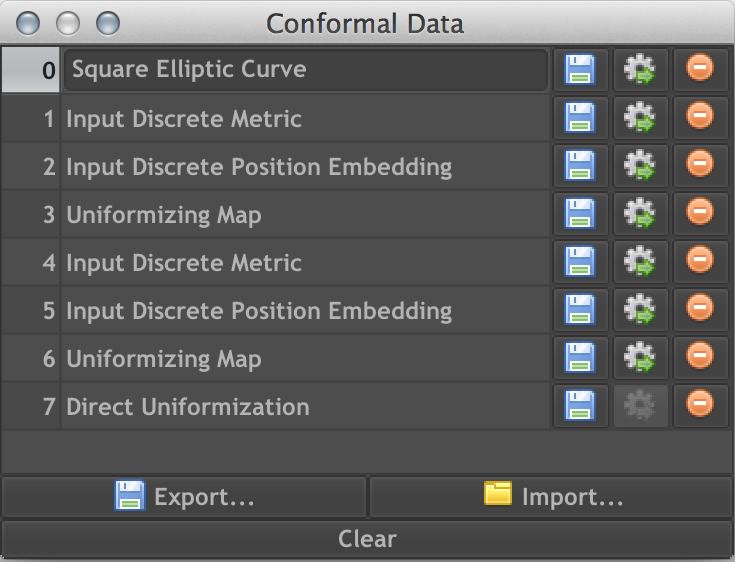
\includegraphics[width=\linewidth]{conformllab/conformal_data.png}
\caption{XML data import and export interface of {\sc ConformalLab}.}
\label{fig:conformal_data}
\end{wrapfigure}
The data import and export panel, see Figure~\ref{fig:conformal_data},
provides functions to import and export data as described in Section~\ref{sec:conformal_data}.
Data can be loaded into memory via the Import button. A table lists the entries of the loaded file.
Loadable are {\tt ConformalDataList} as well as single data instances. The entries of a
{\tt ConformalDataList} are listed in the table of the panel. Each of the rows contains buttons
to save the data to disk (blue disk), load it into the program (gear with green arrow), or delete 
it from the list (red circle).
The function of the load button depends on the data type. A {\tt HalfedgeEmbedding} is
loaded as geometry. A {\tt HalfedgeMap} defined geometry together with texture coordinates
and boundary identifications. If suitable boundary identification is given a uniformizing
group is calculated and visualized.

\begin{wrapfigure}{R}{0.4\textwidth}
\centering
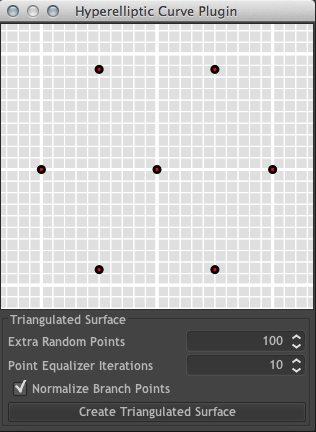
\includegraphics[width=\linewidth]{conformllab/hyperelliptic_curve.png}
\caption{Hyperelliptic curve interface of {\sc ConformalLab}.}
\label{fig:conformal_hyperelliptic}
\end{wrapfigure}

\begin{wrapfigure}{R}{0.4\textwidth}
\centering
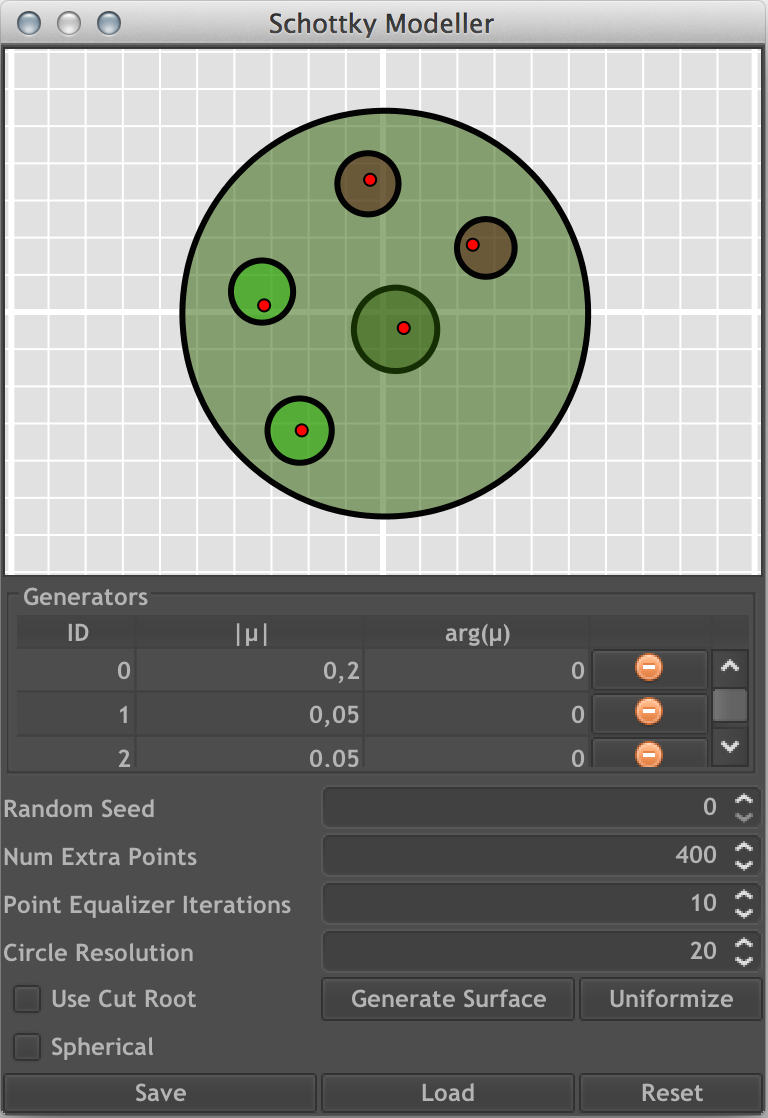
\includegraphics[width=\linewidth]{conformllab/schottky_modeller.png}
\caption{The Schottky modeller user interface of {\sc ConformalLab}.}
\label{fig:conformal_schottky}
\end{wrapfigure}

\begin{wrapfigure}{R}{0.3\textwidth}
\centering
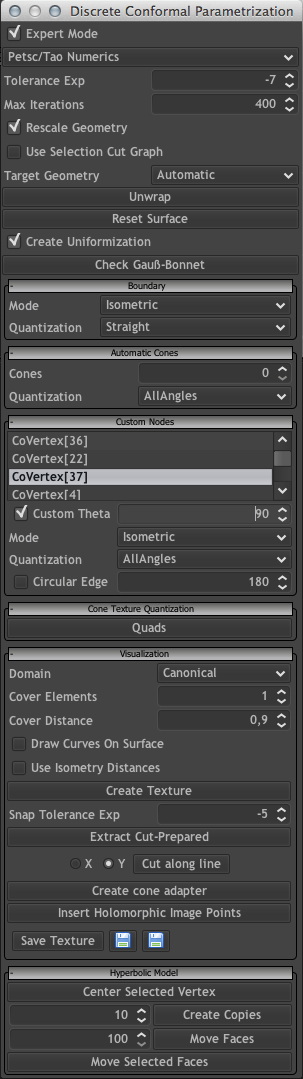
\includegraphics[width=\linewidth]{conformllab/main_interface.png}
\caption{The main interface of {\sc ConformalLab}.}
\label{fig:conformal_main}
\end{wrapfigure}



\subfilebibliography
\end{document}

%%% Local Variables:
%%% TeX-master: "Thesis.tex"
%%% End:
\documentclass[Thesis.tex]{subfiles}
\begin{document}
%\setkeys{Gin}{draft=false}
\chapter{{\sc VaryLab} - Discrete surface optimization}
\label{chp:varylab}

\section{Introduction}

\begin{figure}
    \begin{center}
    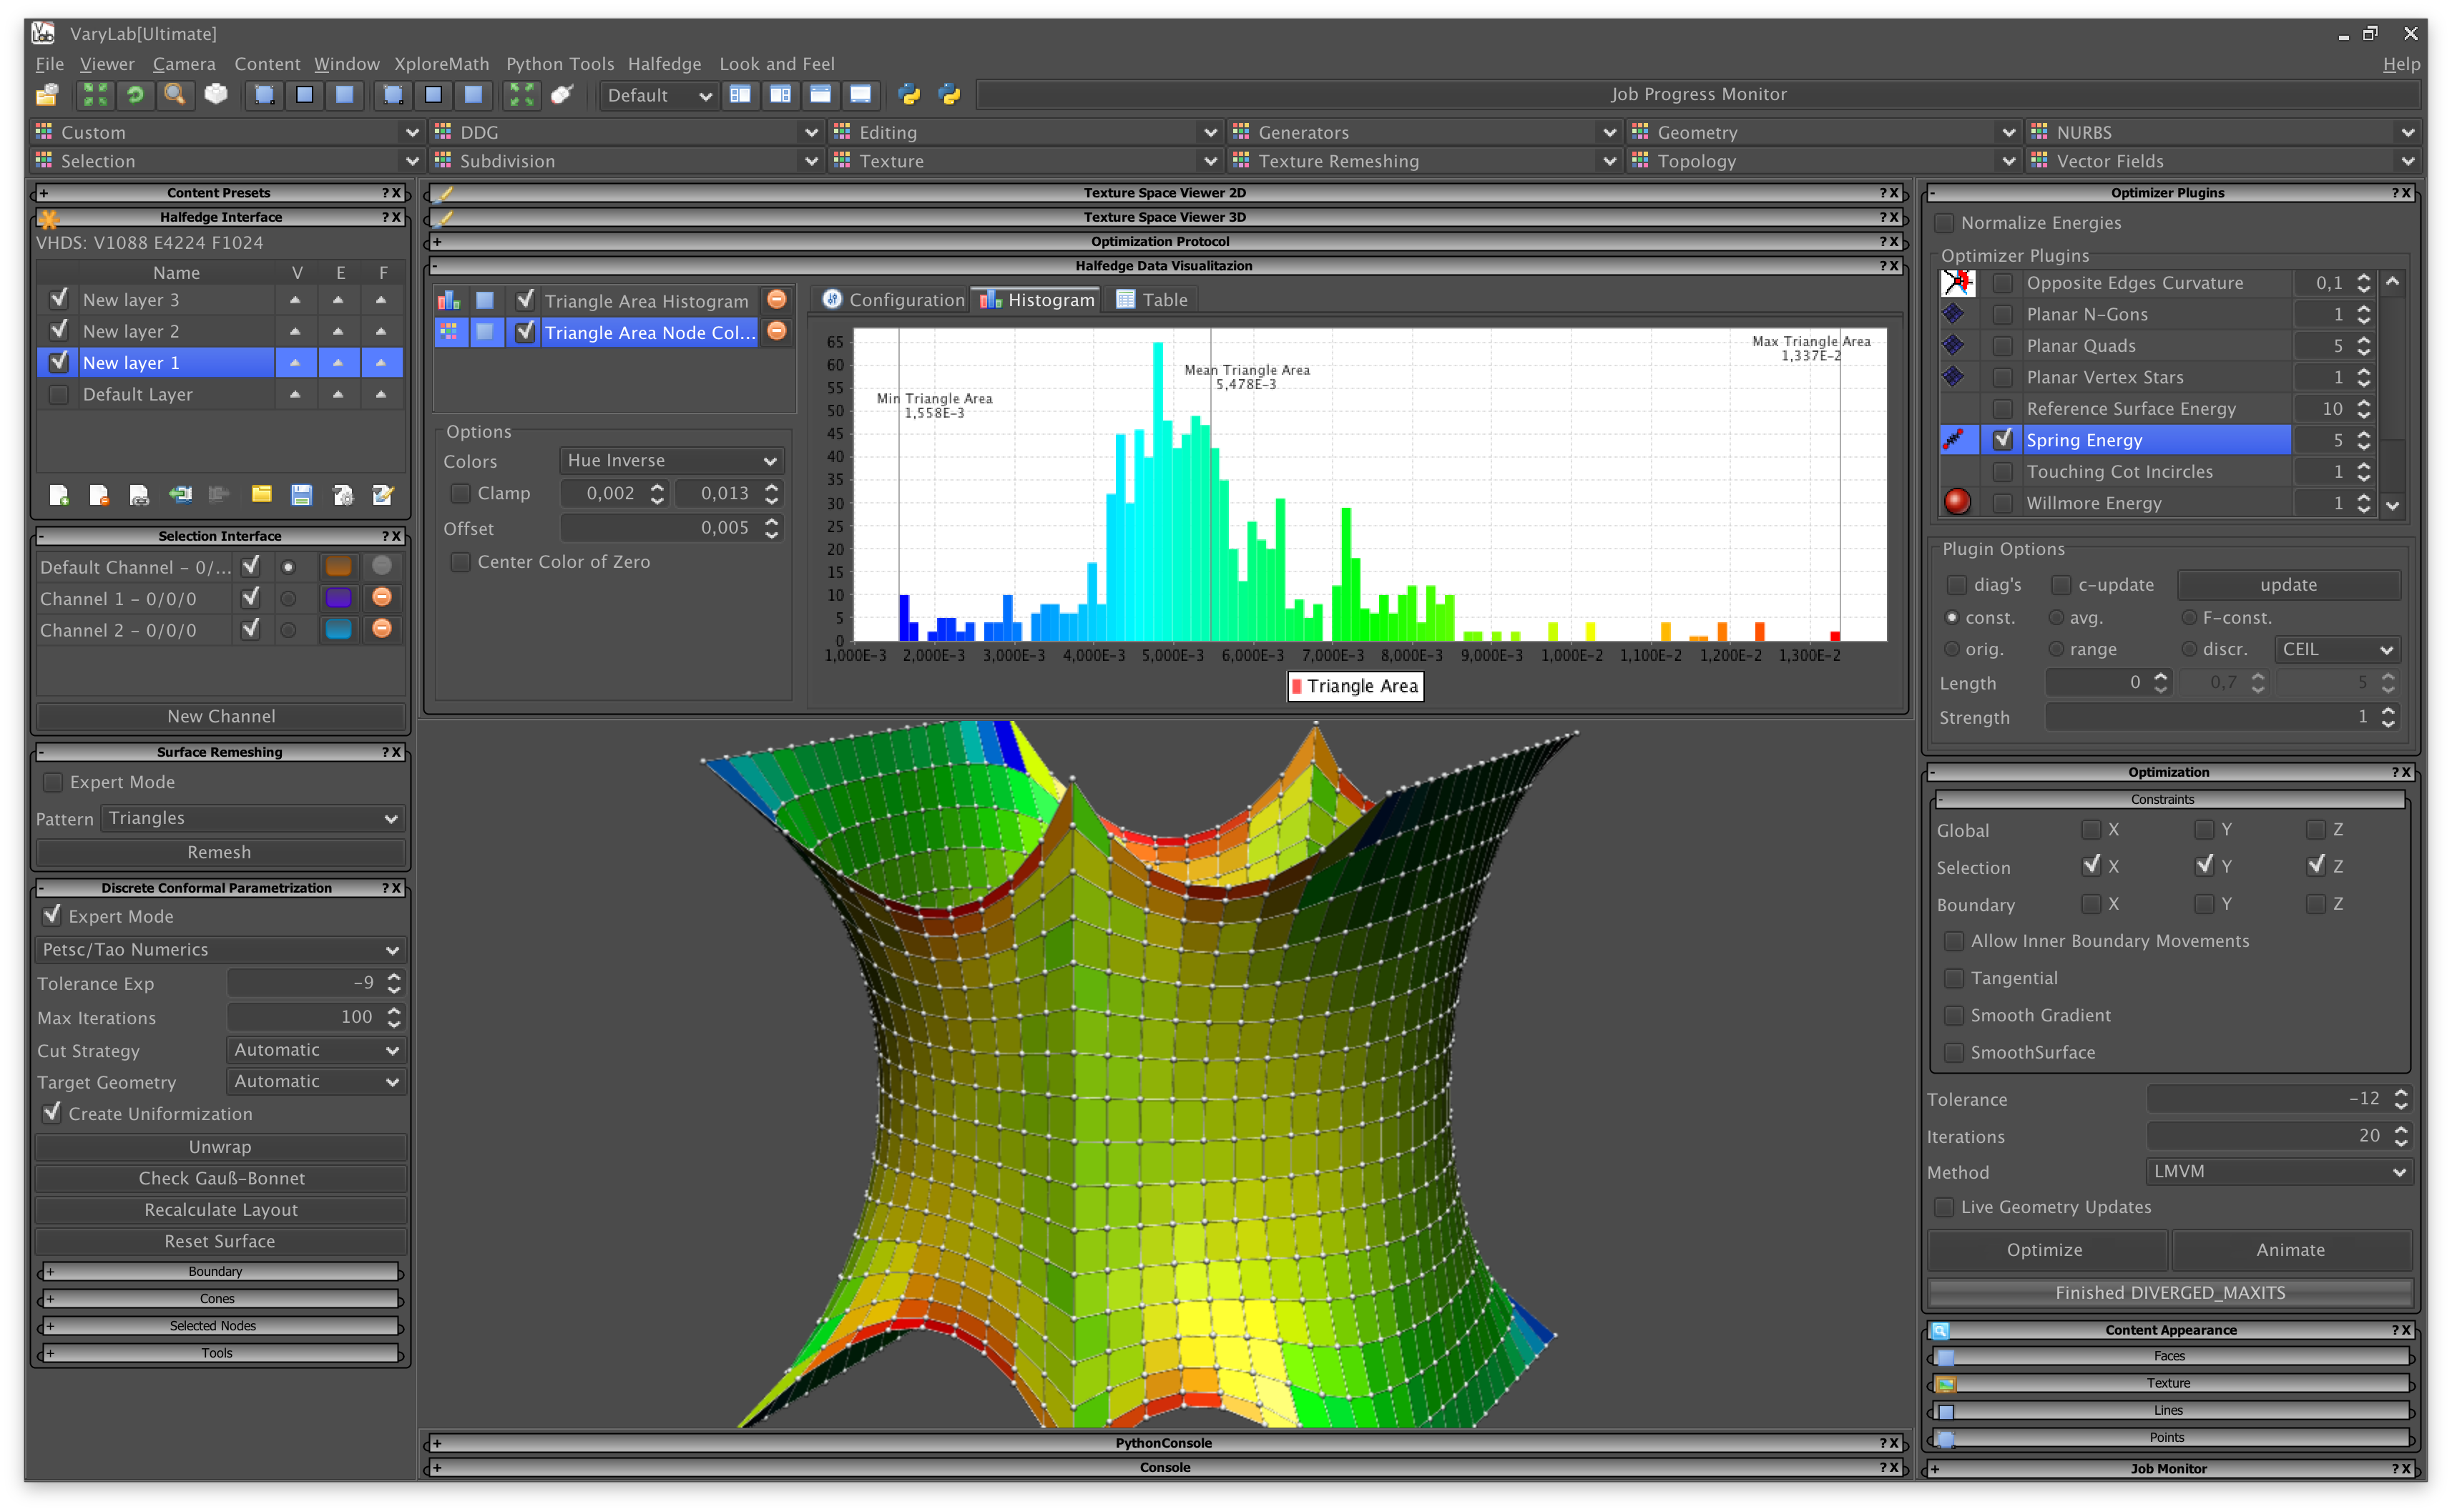
\includegraphics[width=0.8\textwidth]{varylab/varylab_main.png}
    \caption{{\sc VaryLab} main user interface window. Visualization interface (top), energy configuration and optimization tools (right), layers, selections, etc. (left).}
    \label{fig:varylab_main_ui}
    \end{center}
\end{figure}

In this chapter we introduce the {\sc Java} software {\sc VaryLab}. It is a software developed at Berlin Institute of Technology by the author, Thilo R\"orig, and others. It is supported by DFG \mbox{SFB/TRR}~109 Discretization in Geometry and Dynamics. It is designed to be an extensible and modular tool for experiments with discrete surfaces in pure mathematics and applications in industrial geometry. The purpose of this chapter is to enable the reader to reproduce the results presented in Part~\ref{part:applications} of this work.

We start with a general description of {\sc VaryLab} and its features in Section~\ref{sec:general_varylab}. Section~\ref{sec:ui_varylab} introduces the user interface which is based on {\sc JRWorkspace}, see Chapter~\ref{chp:jrworkspace}. Section~\ref{sec:periodic_varylab}, gives details on the use of {\sc VaryLab} when calculating the examples of Chapter~\ref{chp:periodic_conformal_maps}. Section~\ref{sec:quasiisothermic_varylab} explains the steps needed to reproduce results presented in Chapter~ref{chp:quasiisothermic}. Finally, in Section~\ref{sec:gridshells_varylab} we present the capabilities of {\sc VaryLab} when calculating gridshell nets as explained in Chapter~\ref{chp:gridshells}.

In this chapter words in [Brackets] describe ui elements.

\section{Non-linear discrete surface optimization}
\label{sec:general_varylab}
In its core {\sc VaryLab} is a solver for non-linear optimization problems on the coordinates of a given 3D discrete surface. That means given a surface $S$ and functionals $f_1,\ldots,f_n:S\to\R$ we (try to) minimize the combined functional

\begin{eqnarray}
	f(S) = \sum_{i=1}^n \lambda_i f_i(S) \label{eq:varylab_functional}
\end{eqnarray}
where $\lambda_1,\ldots,\lambda_n\in \R$ are user defined weights. Correspondingly the first and second  derivatives of $f_i(S)$ are weighted by $\lambda_i$
\begin{eqnarray}
	\nabla f(S) = \sum_{i=1}^n \lambda_i \nabla f_i(S), \quad \nabla\nabla f(S) = \sum_{i=1}^n \lambda_i \nabla\nabla f_i(S). \label{eq:varylab_derivatives}
\end{eqnarray}

{\sc VaryLab} uses the numerical library {\sc PETSc}/{\sc TAO} \cite{petsc-user-ref, petsc-web-page, tao-user-ref} and the corresponding {\sc Java} bindings \cite{jpetsctao-web-page} for computations. To run optimization methods we need at least an implementation of the functional's value. Other methods need gradient or Hessian of the functional. The most important methods are
 
\begin{tabular}{c | c | c}
	$f$ & $f$, $\nabla f$ & $f$, $\nabla f$, $\nabla\nabla f$\\ \hline
	{\tt NM} Nelder-Mead & {\tt LMVM} Limited-Memory, Variable-Metric & {\tt NLS} Newton Line-Search \\
	& {\tt CG} Conjugate Gradient & {\tt NTR} Newton Trust-Region.
\end{tabular}

In {\sc VaryLab} a functional can choose to implement just the value. Additionally it can implement the gradient and the Hessian of $S$. In principle all methods can be used with all functionals even if those do not implement all data needed for the algorithm. {\sc VaryLab} approximates the values of the gradient or the Hessian if they are missing.

{\sc VaryLab} has the option to normalize the energies before optimization and calculates a $\mu_i$ for each of the energies such that 	$\left\Vert\mu_i\nabla f_i(S)\right\Vert = 1$ for each functional $f_i$ and for the current mesh geometry. Then it uses a modified energy
\begin{eqnarray}
	\hat{\mathit f}(S) = \sum_{i=1}^n \mu_i\lambda_i f_i(S). \label{eq:varylab_normalized_functional}
\end{eqnarray}
for optimization.

{\sc VaryLab} can handle constraints on vertex positions. We implement this by modifying the gradient and Hessian of the selected energies to be zero at the constraint variables. Even if the derivative does not match the energy anymore we can still calculate solutions for the rest of the variables using conjugate gradient methods. Here the line search step of the algorithm minimizes the energy over the remaining variables in the direction of the gradient, i.e., the update will not include constraint variables.

\section{Build-in Functionals}

{\sc VaryLab} implements a number of energy functionals.

\begin{itemize}
\item \emph{Circular Quadrilaterals Energy} - Defines an energy functional which is minimal for planar circular quads. Since we are using an angle criterion, the convergence to planarity is relatively slow. If the planar quads energy is added to the optimization, the geometry converges more quickly.
\item \emph{Conical Quadrilaterals Energy} - This energy implements an angle criterion for conical meshes. So in combination with planarity it optimizes a mesh to have the property, that faces adjacent to one node are tangent to a cone of revolution.
\item \emph{Cotangent Dirichlet Energy} - Dirichlet energy for the three coordinate functions of vertices of a triangle mesh. Edge weights are defined as $\omega_\mathit{ij}=\frac{1}{2}(\cot\alpha_\mathit{ij}+\cot\alpha_\mathit{ji})$ where $\alpha_\mathit{ij}$ and $\alpha_\mathit{ji}$ are the angles opposite of the edge $e_\mathit{ij}$.
\item Equal Edge Lengths
\item \emph{Incircles} - The property for a quadrilateral to possess an incircle tangent to its sides is that the two sums of opposite side lengths is equal $a+c=b+d$. Planarity is not included in this functional, so to get planar quadrilaterals with inscribed incircles you need to add planarity to the optimization.
\item \emph{Touching Incircles} - In a quad-mesh with incircles, the incircles need not touch. So in combination with the incircles and planarity energies it one can create a mesh with touching incircles.
\item \emph{Opposite Edges Curvature} - This energy penalizes the deviation of a parameter polyline from a straight line. So using this energy only, will flatten the mesh to the plane. Used together with, e.g., a reference surface energy, this energy smoothes the  parameter lines of the quad mesh.
\item \emph{Opposite Angles Curvature} - This curvature is based on the intrinsic geometry of the surface. Let $\alpha$, $\beta$, $\gamma$, and $\delta$ denote the angles in the adjacent quads at a node in cyclic order. Then the optimal mesh satisfies $\alpha+\beta=\gamma+\delta$ and $\beta+\gamma=\delta+\alpha$, i.e., the parameter lines are straight from an intrinsic point of view.
\item \emph{Planar Quadrilaterals} - Energy that enforces planarity of quadrilaterals. Implemented either as the distance of the diagonals or as the determinant of the four homogeneous vertex coordinates.
\item \emph{Planar $n$-gons} - Generalization of the energy for planar quadrilaterals. Implemented as the sum of all choices of four vertices in each face.
\item \emph{Planar Vertex Stars} - This energy is dual to the planar faces energy. It computes the volume spanned by a node and its neighbors. Minimization yields meshes such that each node lies in a plane with its neighbors. If used together with face planarity the initial mesh is mapped to a plane.
\item \emph{Reference Mesh} - Given a reference mesh we compute the closest point to a node and add a spring force between each node and its projection. The projection point is recomputed in each step of the optimization. If combined with other energies it keeps the optimized mesh close to a reference mesh.
\item \emph{Spring Energy} - The spring energy is computed by adding springs to all the edges of the mesh. These springs can have user specified target lengths and strengths that can be specified by various options.
\end{itemize}

\section{Geometry Processing}

The geometry processing core of {\sc VaryLab} is based on {\sc HalfEdge} and {\sc HalfEdgeTools} (Chapter~\ref{chp:halfedge}), i.e., all geometry processing is done with the help of the half-edge data structure and algorithms that run on top of it. Frequently used geometry processing features include

\begin{figure}
    \begin{center}
    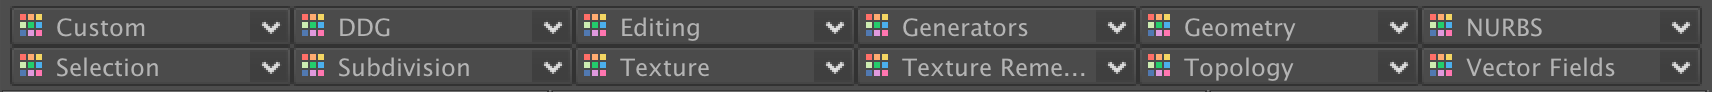
\includegraphics[width=\textwidth]{varylab/tools.png}
    \caption{{\sc VaryLab} tools tool bar.}
    \label{fig:varylab_tools_ui}
    \end{center}
\end{figure}

\begin{itemize}
\item Mesh Generators - Regular Planar Meshes, Convex Hull, Primitive Meshes such as cube, cylinder, sphere, etc.
\item Mesh Editing - Vertex/Edge/Face operations based on user selection.
\item Subdivision - CatmullClark, Doo Sabin, Loop, Sqrt3, etc.
\item Remeshing - Quadritalerals, Triangles, Singularties.
\end{itemize}

All tools are available via the tools tool bar at the top of the main window, see Figure~\ref{fig:varylab_main_ui} and~\ref{fig:varylab_tools_ui}.

\section{Data Visualization}

{\sc VaryLab} adds data sources corresponding to the energies of the optimization core. Their data can be visualized on the surface using the [Halfedge Data Visualization] interface, see Section~\ref{sec:halfedge_tools_visualization}. 

\begin{figure}
    \begin{center}
    \resizebox{\textwidth}{!}{
        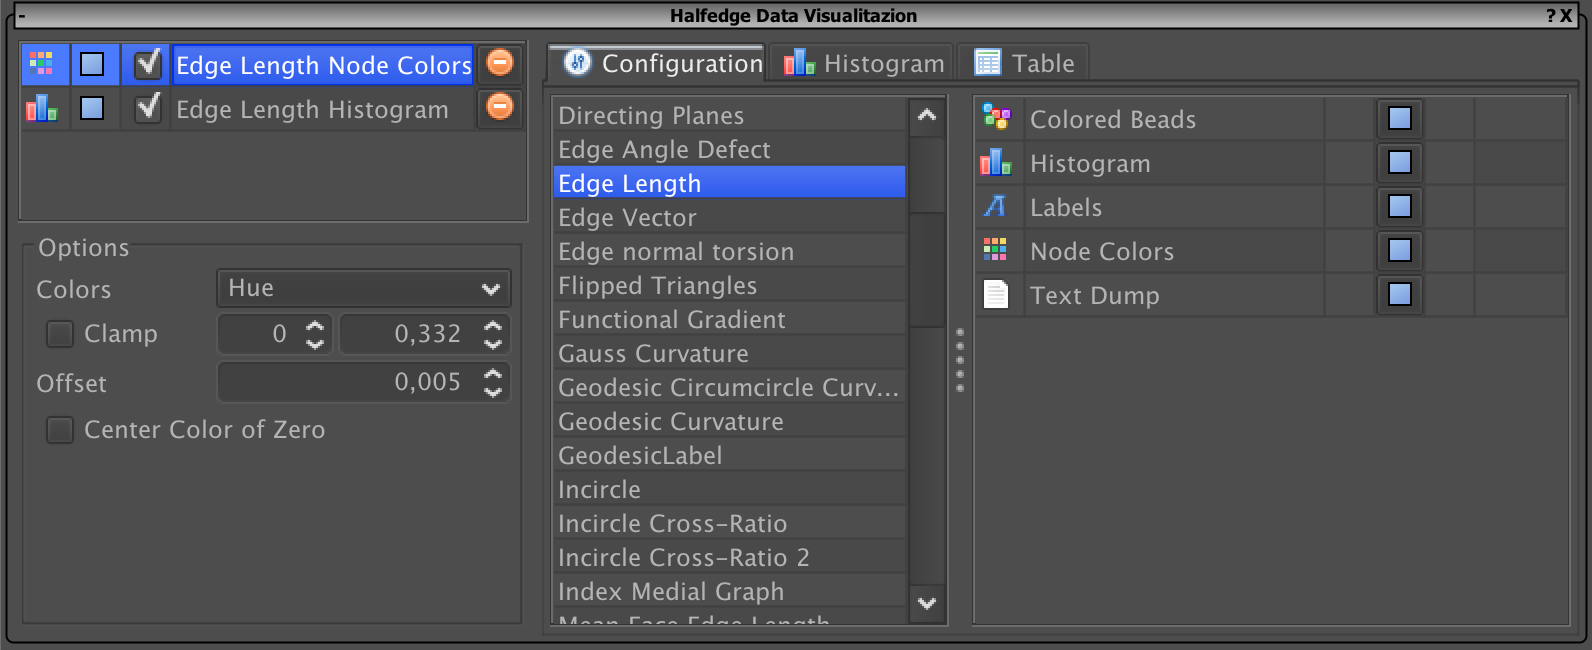
\includegraphics[width=\textwidth]{varylab/edge_visualization.png}
        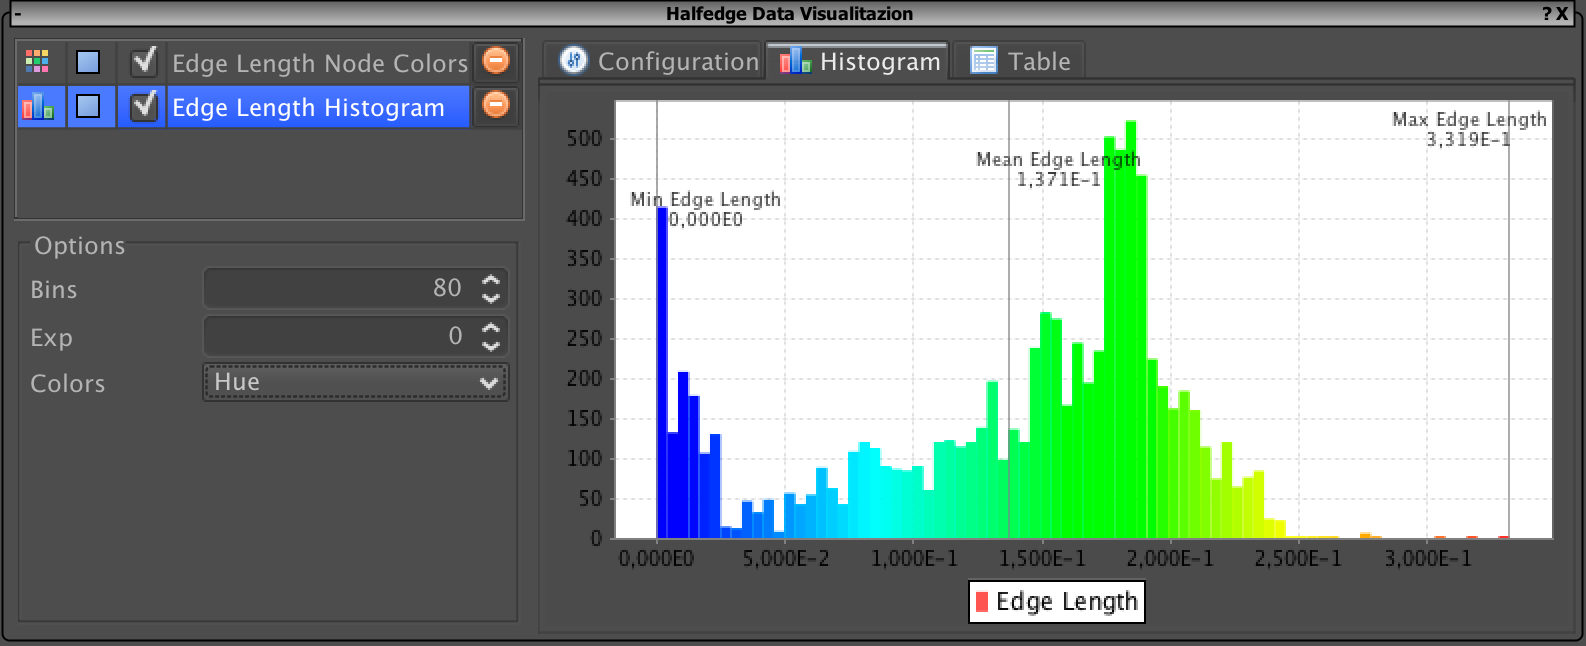
\includegraphics[width=\textwidth]{varylab/edge_histogram.png}    
    }
    \caption{Visualization interface (left), Visualizing mesh edge length data as node colors on a surface and as histogram (right).}
    \label{fig:visualizing_edge_lengths}
    \end{center}
\end{figure}

\begin{example}[Analyzing edge length density] Load some mesh geometry. In the [Halfedge Data Visualization] select the [Edge Length] data source. It provides scalar data for edges of the mesh. Select the [Histogram] and [Node Colors] visualizers to create colored edges and a corresponding histogram for the edge lengths of the mesh, see Figure~\ref{fig:visualizing_edge_lengths}.
\end{example}

\setkeys{Gin}{draft=true}

%Derivatives and numerical substitutes, 
%Boundary Conditions
%Numerics
%Build-In Functionals
%Plug-in facility and extensibility, 
%Data Visualization (scalar, vector)
%Remeshing

\section{User interface}
\label{sec:ui_varylab}

The user interface of {\sc VaryLab}, see Figure~\ref{fig:varylab_main_ui}, is based on {\sc JRWorkspace}, Chapter~\ref{chp:jrworkspace}. Thus it inherits the ability for the user to freely move around all interface components of the main window, see Figure~\ref{fig:varylab_main_ui}. 
The three most important interface components are shown in Figure~\ref{fig:optimization_interface_varylab} and \ref{fig:protocol_interface_varylab}. It is the list of energies, the optimization controls, and the optimization protocol.

\begin{figure}
\begin{center}
    \resizebox{\linewidth}{!}{
        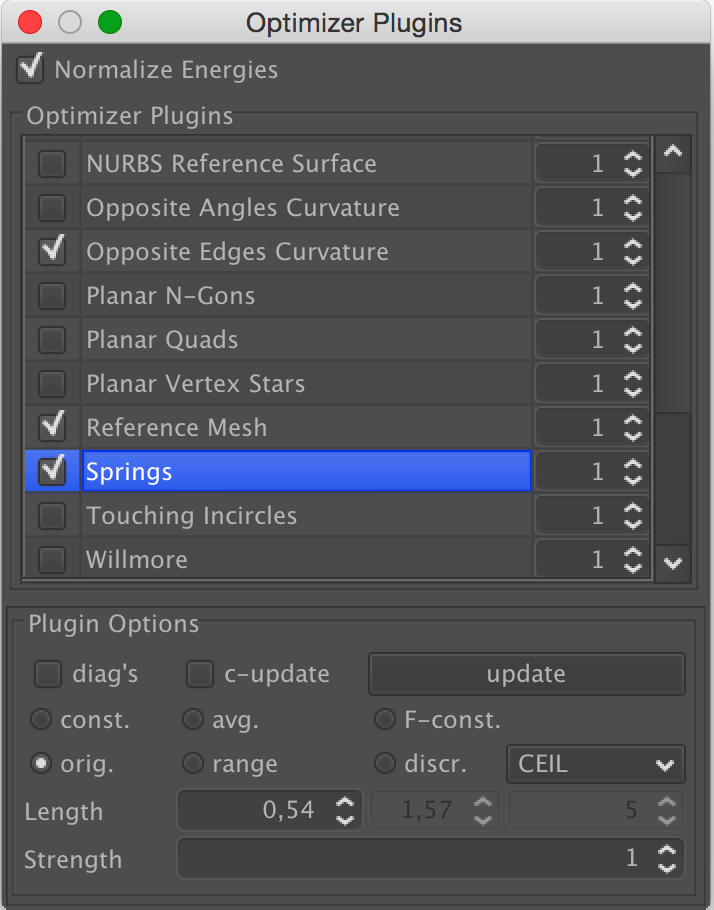
\includegraphics[width=\textwidth]{varylab/optimization_plugins2.png}
        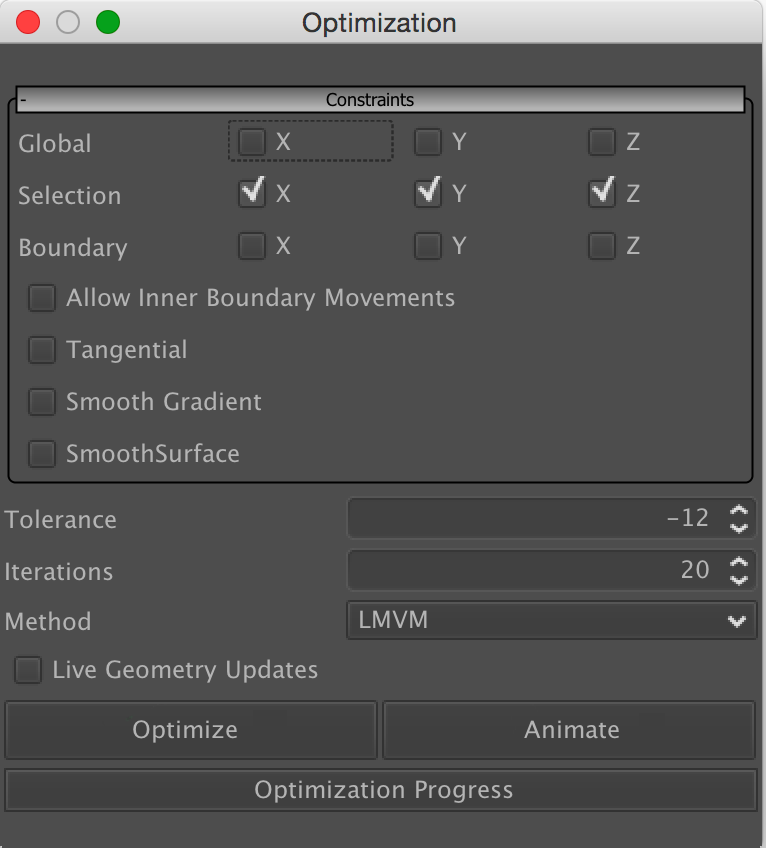
\includegraphics[width=\linewidth]{varylab/optimization2.png}
    }
\caption{The main user interface panels of {\sc VaryLab}. List of optimization functional plug-ins and their options (left). Main optimization controls with global constraints and minimizer settings (right).}
\label{fig:optimization_interface_varylab}
\end{center}
\end{figure}

\subsection*{Optimizer Plug-ins Panel}
The [Optimizer Plugins] panel, see Figure~\ref{fig:optimization_interface_varylab} (left), has a list with all currently loaded plug-ins that implement energies for the use with the non-linear optimization core. For each energy one can adjust the coefficient $\lambda$ in the sum of functionals, see Equation~(\ref{eq:varylab_functional}).
The checkbox [Normalize Energies] activates normalization of energies, see Equation~(\ref{eq:varylab_normalized_functional}). For a selected energy options are displayed right under the table.

\subsection*{Optimization Panel}
In the [Optimization Panel], see Figure~\ref{fig:optimization_interface_varylab} (right), we can configure constraints and run the optimization. Vertices can be fixed either globally in one or all coordinate directions, by selection, or as boundary constraint. Constraints are handled as described in Section~\ref{sec:general_varylab}

The check box [Allow Inner Boundary Movement] is used in conjunction with boundary constraints. The corresponding gradient part is projected onto an adjacent boundary edge thus any conjugate gradient update will move the vertex along this direction. This mode is meant to be used with straight boundaries, otherwise the behavior is undefined.

Analogously to the inner boundary movement constraint the [Tangential]
 constraint projects the gradient of a vertex onto the tangent plane at this vertex for current mesh geometry. With this options vertices stay close to the initial surface if the surface is sufficiently smooth but can move freely along tangent directions of the surface.

The options [Smooth Gradient] and [Smooth Surface] apply Laplacian smoothing to either the gradient or the coordinate values of the mesh. We use a graph Laplacian, i.e., all weights are one.

The values for [Tolerance] and [Iterations] define stop criteria for the optimization core. If the Frobenius norm of the gradient drops below the tolerance or if the maximum number of iterations are performed the optimizer stops. 

The numerical [Method] can be selected from the drop down field, see Section~\ref{sec:general_varylab} for explanation.

The check box [Live Geometry Updates] updates the coordinates of the surface during optimization if selected. Any visualization is updated accordingly.

\subsection*{Optimization Protocol Panel}

During optimization {\sc VaryLab} logs the energy of each functional as well as the Frobenius norm of the gradient and plots them to the optimization protocol, see Figure~\ref{fig:protocol_interface_varylab}. The energy value is drawn as a green curve, the norm of the gradient is a purple curve. By default the display is logarithmic in the values and linear in time.


\begin{figure}
\begin{center}
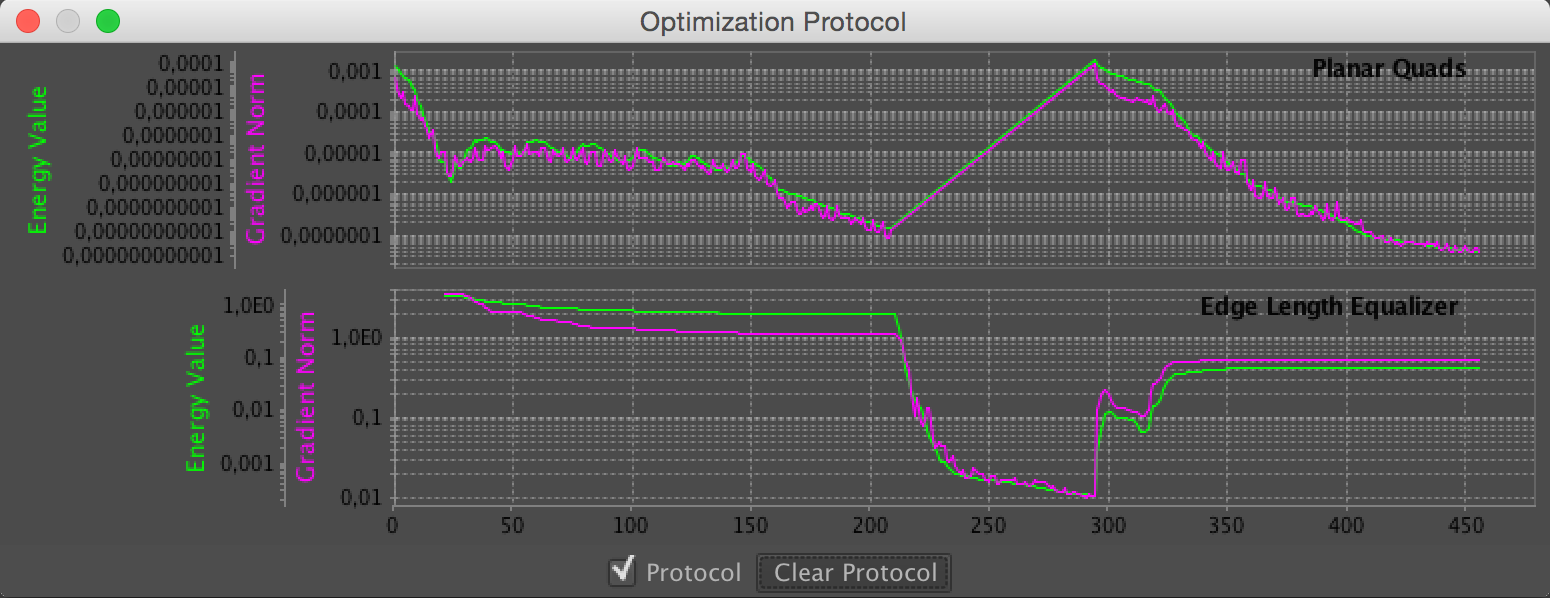
\includegraphics[width=\textwidth]{varylab/protocol.png}
\caption{Optimization protocol panel shows the progress of the optimization for each activated energy in the Optimizer Plug-ins panel, see Figure~\ref{fig:optimization_interface_varylab} (left).}
\label{fig:protocol_interface_varylab}
\end{center}
\end{figure}

\setkeys{Gin}{draft=true}

\section{Periodic conformal maps with {\sc VaryLab}}
\label{sec:periodic_varylab}
In this section we describe how the methods of Chapter~\ref{chp:periodic_conformal_maps} are implemented in {\sc VaryLab}. We split the process in two parts. Part one describes the creation of periodic triangle, quad, or hexagonal meshes from an initial unstructured triangle mesh. Part two deals with optimization of panels created from a mesh in part one.

\subsection{Periodic Parameterization}
The parameterization part of the work is carried out via the {\sc ConformalLab} main user interface. 

\begin{itemize}
\item[0] Load a surface with two boundary components. You can map the surface using the three methods described in the article, map to a cylinder (a), polygonal map to a cone of revolution (b), and isometric boundary (c) to an adapted cone of revolution.
\item[1(a)] For the map to the cylinder create a conformal parameterization with straight boundary using the [Discrete Conformal Parameterization] panel and [Quantized Angles/Straight] boundary mode. A cut is introduced automatically to uniquely define the map.\\

\begin{center}
\begin{minipage}{0.9\linewidth}
            \centering
            \resizebox{\linewidth}{!}{
            	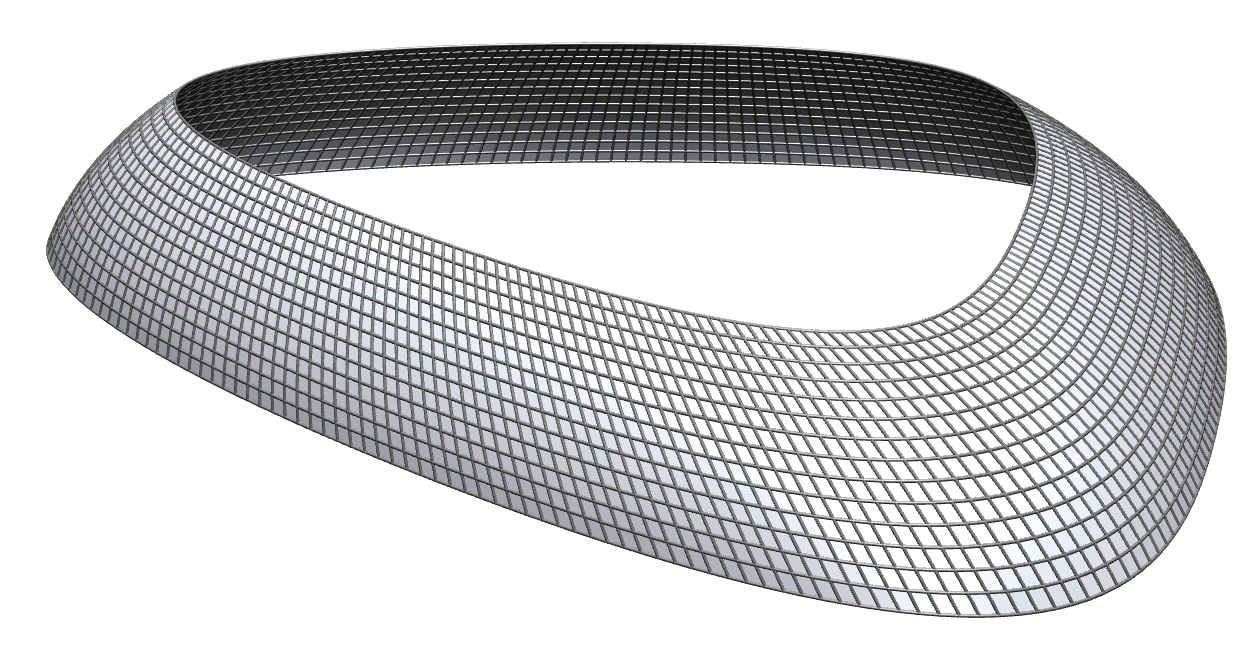
\includegraphics{periodic/step00.png}
            	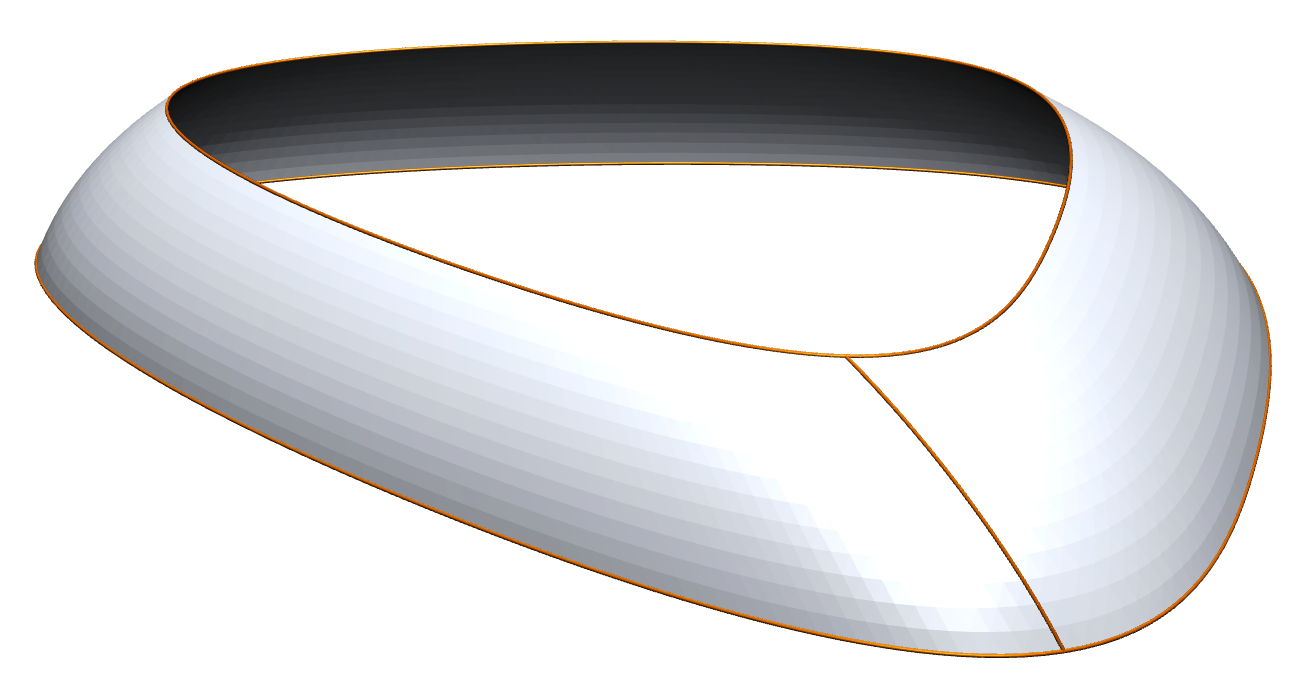
\includegraphics{periodic/step01_surface.png}	
            	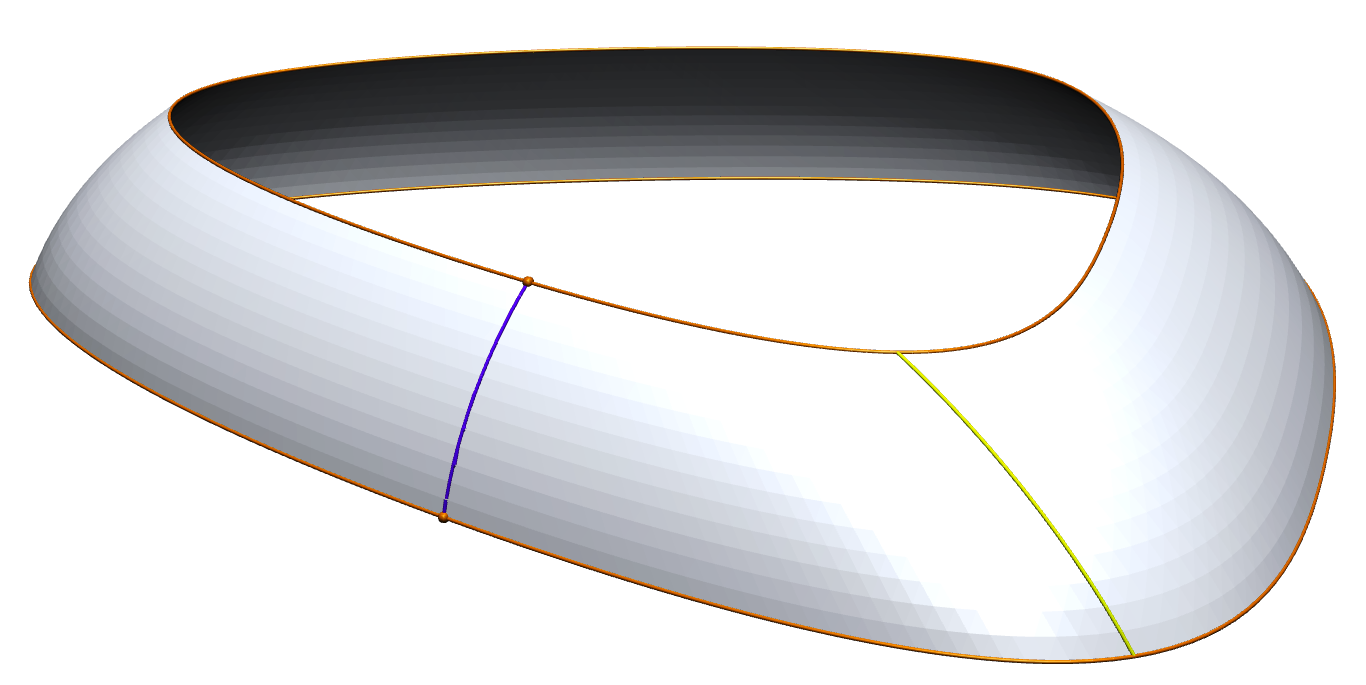
\includegraphics{periodic/step02_surface.png}		
            }
            \resizebox{\linewidth}{!}{
                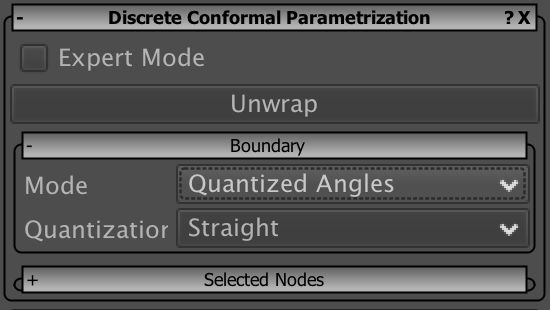
\includegraphics[width=3.2cm]{periodic/step01_ui.png}
                \begin{minipage}[b]{10cm}
                    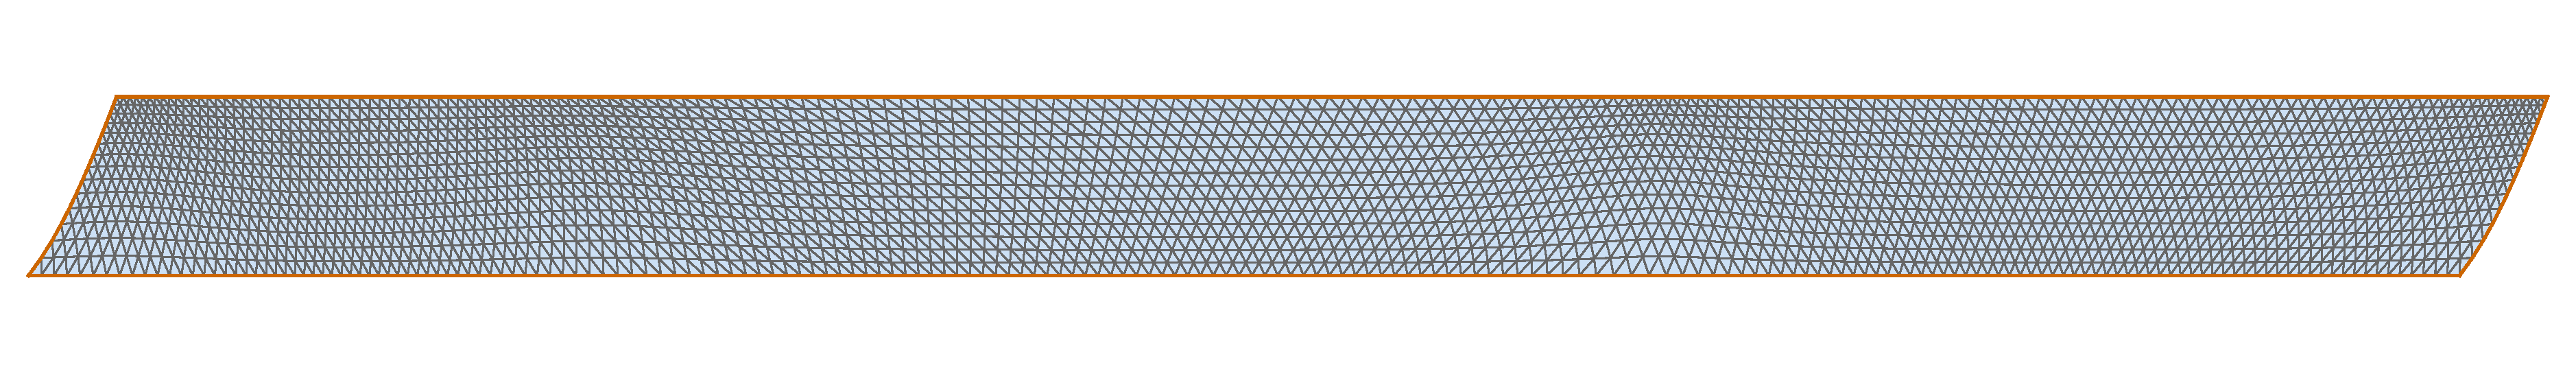
\includegraphics[width=\linewidth]{periodic/step01a_map.pdf}\\
                    \includegraphics[width=\linewidth]{periodic/step02a_map.pdf}
                \end{minipage}
            }
            \captionof{figure}{Map to cylinder. Start with an automatically cut mesh (top-middle and upper domain image) and modify the cut (top-right and lower domain image) such that the remeshing algorithm can handle the complete boundary.}
            \label{fig:periodic_algorithm1a}
\end{minipage}
\end{center}            

\item[1(b)] For a polygonal map to a cone of revolution, select boundary vertices to specify boundary angles for the domain. Use multiples of $\frac{\pi}{3}$ for triangle/hexagonal panels and multiples of $\frac{\pi}{4}$ for quadrilaterals.

\begin{center}
\begin{minipage}{0.9\linewidth}
            \centering
            \resizebox{0.7\textwidth}{!}{
            	\includegraphics{periodic/step01b_map.pdf}
            	\includegraphics{periodic/step02b_map.pdf}	
            }
            \captionof{figure}{Mapping the surface from Figure~\ref{fig:periodic_algorithm1a} to a hex pattern adapted domain with polygonal boundary curve. Cut orthogonal to the boundary to create a domain that can easily be meshed with boundary aligned hexagons. The domain is identified along the cut via a rotation by $\pi$.}
\end{minipage}
\end{center}

\item[1(c)] Create an isometric boundary and a map to cone of revolution using the [Read Isometric Angles] boundary mode and the [NoCuts] cut strategy. It creates a map to an arbitrary cone of revolution and reads off the resulting boundary angles. Those are set as new boundary conditions (red vertex selection). In a second step choose the [Quantized Angle Periods] boundary mode and the desired quantization for the final map to the pattern adapted cone of revolution.

\begin{center}
\begin{minipage}{0.9\linewidth}
            \centering
            \resizebox{\linewidth}{!}{
            	\includegraphics[width=5cm]{periodic/step01c_map.pdf}
            	\includegraphics[width=5cm]{periodic/step02c_map_hexadapted.pdf}	
            	\includegraphics[width=6cm]{periodic/step02c_surface.png}		
            }
            \captionof{figure}{Map to cylinder with isometric boundary. Create a map with isometric boundary without cutting the mesh (left). Modify the resulting boundary angles to support a periodic pattern (middle). Periodic hexagonal pattern on the surface (right)}
\end{minipage}
\end{center}    

\item[2] Use the [Cut and Glue Texture Domain] command and select [Orthogonal to Boundary] to create a map to a rectangle (a), a map to a polygonal region (b). In the isometric boundary case (c) we do not need a polygon as boundary curve.
\item[3] Select a predefined texture for quadrilateral, triangle, or hexagonal mesh preview from the [Content Appearance$\to$Texture] panel. Adjust the texture scale to a reasonable value. In the isometric case (c) close the period with the texture transformation user interface manually. For cases (a) and (b) periods will be closed automatically by the remeshing algorithm.

\begin{center}
\begin{minipage}{0.9\linewidth}
            \centering
            \resizebox{\linewidth}{!}{
            	\includegraphics[width=5cm]{periodic/step03_quads.png}
            	\includegraphics[width=5cm]{periodic/step03_triangles.png}	
            	\includegraphics[width=1.5cm]{periodic/step03_ui.png}	
            }
            \captionof{figure}{Pattern preview.}
\end{minipage}
\end{center}    

\item[4] Perform remeshing in cases (a) and (b) either for [Boundary Aligned Triangles] or [Boundary Aligned Quads] using the [Surface Remeshing] panel. For non-boundary aligned parameterization (c) use the [Quads With Singularities/Triangles With Singularities] remeshing mode.\\

\begin{center}
\begin{minipage}{0.9\linewidth}
            \centering
            \resizebox{\linewidth}{!}{
            	\includegraphics[width=5cm]{periodic/step04_quads_surface.png}
            	\includegraphics[width=5cm]{periodic/step04_triangles_surface.png}	
            	\includegraphics[width=2cm]{periodic/step04_ui.png}	
            }
            \includegraphics[width=\linewidth]{periodic/step04_quads_map.pdf}
            \includegraphics[width=\linewidth]{periodic/step04_triangles_map.pdf}
            \captionof{figure}{New mesh and domain.}
\end{minipage}
\end{center}    

\item[5] Create a watertight mesh using the [Watertight Mesh Generator] and remove extra edges and vertices. In the isometric case (c) use a combination of [Topology$\to$Stitch] and [Topology$\to$Stitch Cut Path] to remove the cut path from the mesh.
\item[6] For hexagonal mesh creation select from the periodic triangle mesh all centers of hexagons using the [Selection$\to$Lattice] command. The [Remove Vertex and Fill] command then creates a periodic hexagonal mesh.
\begin{center}
\begin{minipage}{0.9\linewidth}
            \centering
            \resizebox{\linewidth}{!}{
            	\includegraphics{periodic/step05.png}
            	\includegraphics{periodic/step06.png}
            	\includegraphics{periodic/step07.png}	
            }
            \captionof{figure}{Creating a periodic hexagonal mesh from a triangle mesh.}
\end{minipage}
\end{center}                
\end{itemize}

\subsection{Panel optimization}

\begin{itemize}
\item[8] [Topology]$\to$[Explode] creates separate faces. Use a [Mean face Edge Length] histogram to show the density of edge lengths. If you want planar panels you should planarize them now.

\begin{center}
\begin{minipage}{0.9\linewidth}
            \centering
            \resizebox{\linewidth}{!}{
            	\includegraphics[width=5cm]{periodic/step08_surface.png}
            	\includegraphics[width=5cm]{periodic/step08_histogram.png}		
            }
            \captionof{figure}{Measuring panel sizes and density with the [Halfedge Data Visualization] facility.}
\end{minipage}
\end{center}

\item[9] Equalize the edge lengths per face using the [Springs] Energy and [F-const] option. Use the [Floor] rounding method. Press [Update] to set target lengths per face.

\begin{center}
\begin{minipage}{0.9\linewidth}
            \centering
            \resizebox{\linewidth}{!}{
            	\includegraphics[width=13cm]{periodic/step09_surface.png}
            	\includegraphics[width=5cm]{periodic/step09_fconst.png}
            }
            \captionof{figure}{Creating regular elements with the [Spring] energy.}
\end{minipage}
\end{center}
\item[10] From the histogram read off the smallest and largest edge lengths and transfer those into the [Springs] energy ui. Select the [discr.] option and the number of discrete steps. Optimize the surface to consist of a limited number of panel sizes.

\begin{center}
\begin{minipage}{0.9\linewidth}
            \centering
            \resizebox{\linewidth}{!}{
            	\includegraphics[width=13cm]{periodic/step11_surface1.png}
            	\includegraphics[width=5cm]{periodic/step10_springs.png}
            }
            \captionof{figure}{Optimization towards a discrete set of panel sizes.}
\end{minipage}
\end{center}            
\end{itemize}



\section{Quasiisothermic meshes with {\sc VaryLab}}
\label{sec:quasiisothermic_varylab}

The methods of Chapter~\ref{chp:quasiisothermic} can be divided into two parts. The Parameterization part where we create the coordinates of the triangle mesh based on curvature direction data on the boundary of the mesh. And the optimization part where a quadrilateral mesh from part 1 is optimized towards touching incircles, the defining property of discrete s-isothermic meshes.

\subsection{Quasiisothermic paramerization}

\begin{itemize}
\item[0] Load a genus $0$ surface with one boundary component.
\item[1] Calculate curvature direction estimates on interior vertices to find singularity locations and indices with the [Vector Field$\to$Curvature Vector Fields] command. Visualize directions using the [Halfedge Data Visualization] interface. The data is called, e.g., [Kmax Vec V] for maximum curvature direction with respect to the surface normal.
\item[2] Select singularity vertices and assign corresponding cone angles in the [Selected Nodes] panel of the [Discrete Conformal Parameterization] panel.
\item[3] Calculate curvature direction estimates on boundary edges of the surface, again using the [Vector Field$\to$Curvature Vector Fields] command. Check singularity indices with the [Check Gau{\ss}-Bonnet] button in the [Discrete Conformal Parameterization] panel. It prints the left side of the Gau{\ss}-Bonnet equation to the console. It should give $2\pi$ for a genus $0$ surface in this case.

\begin{center}
\begin{minipage}{0.9\linewidth}
            \centering
            \resizebox{\linewidth}{!}{
                \includegraphics[width=5cm]{quasiisothermic/step00.png}
                %\includegraphics[width=5cm]{quasiisothermic/step01.png}
                \includegraphics[width=5cm]{quasiisothermic/step02_surface.png}
                \includegraphics[width=2.6cm]{quasiisothermic/step02_ui.png}
                \includegraphics[width=5cm]{quasiisothermic/step03_surface.png}
            }
            \captionof{figure}{Inspecting the curvature direction field on the surface (middle) and specify boundary conditions (right, magenta) and singularities (right, yellow).}
\end{minipage}
\end{center}     
            
\item[4] Create a discrete conformal parameterization. Use [Conformal Curvature] as boundary mode. Select a quad texture to visualize the parameterization on the surface. Rotate the texture to match the prescribed boundary directions.
\item[5] Move the texture such that singularities lie either in the middle or at a corner of a quad of the texture. Use the [Texture Remeshing$\to$Transform Texture] command to transform the texture such that two selected vertices lie on $(0,0)$ and $(1,0)$ respectively. This method woks for one or two singularities. We do not implement methods to distort the mapping to match more that two singularities.

\begin{center}
\begin{minipage}{0.9\linewidth}
            \centering
            \resizebox{\linewidth}{!}{
                \includegraphics[width=5cm]{quasiisothermic/step04_surface.png}
                \includegraphics[width=4cm]{quasiisothermic/step04_map.pdf}
                \includegraphics[width=5cm]{quasiisothermic/step05_surface.png}
            }
            \captionof{figure}{A quasiisothermic parameterization and its domain (left and middle). Move the singularity to a symmetry point of the pattern to close the parameter lines on the surface.}
\end{minipage}
\end{center}     
            
\item[6] Create a subdivision quad-mesh using the [Surface Remeshing] panel and the [Quads With Singularities] mode. This mode is available in the [Expert] mode of the panel. Press the [Lift/Flat] button to lift the subdivision to the surface.
\item[7] Use the [Texture Remeshing$\to$TextureGeometry] command to extract a quad mesh from the subdivision mesh. Disable the layer of the original mesh as we will continue to work with the quad-mesh.

\begin{center}
\begin{minipage}{0.9\linewidth}
            \centering
            \resizebox{\linewidth}{!}{
                \includegraphics[width=4cm]{quasiisothermic/step06_ui.png}
                \includegraphics[width=4cm]{quasiisothermic/step06_flat_rotate.png}
                \includegraphics[width=5cm]{quasiisothermic/step06_surface.png}
                \includegraphics[width=5cm]{quasiisothermic/step07_surface.png}
            }
            \captionof{figure}{Three-step remeshing of the parameterized surface. Create a subdivided domain (second to left), lift this mesh to the surface (middle). Extract the new mesh from the subdivided (right).}
\end{minipage}
\end{center}                 
            
\item[8] Sew up the path from the boundary to the singularity using the [Topology$\to$ Stitch Cut Path] command. Select the two boundary vertices and a connected edge on the path.
\item[9] Remove extra vertices with the [Texture Remeshing$\to$Collapse 1,2-Valent Vertices] command.
\item[10] Clean up the mesh from extra edges and vertices with the [Selection$\to$Geodesic], [Edit$\to$Remove Edge And Fill], and [Texture Remeshing$\to$Collapse 1,2-Valent Vertices] command.

\begin{center}
\begin{minipage}{0.9\linewidth}
            \centering
            \resizebox{\linewidth}{!}{
                \includegraphics[width=3cm]{quasiisothermic/step08_selection.png}
                \includegraphics[width=3cm]{quasiisothermic/step09.png}
                \includegraphics[width=3cm]{quasiisothermic/step10_selection.png}
                \includegraphics[width=5cm]{quasiisothermic/step10_surface.png}
            }
            \captionof{figure}{Removing the cut from a singularity to the boundary. Stitch the cut path by selecting the two vertices on the boundary and one adjacent edge on the path (left). Remove resulting vertices of valence $2$ (second to left). Select the path and remove extra edges.}
\end{minipage}
\end{center}    
            
\end{itemize}

\subsection{Optimization towards touching incircles}

In Chapter~\ref{chp:quasiisothermic}, Section~\ref{sec:s-isothermic} we propose to further optimize a new mesh to possess touching incircles, i.e., being a discrete s-isothermic mesh by definition. We propose an energy, implemented as [Touching Incircles] energy, that enforces planar quadrilaterals that possess incircles to additionally possess touching incircles. Thus we superpose three energies to achieve the desired effect. Activate [Incircles], [Planar Quads], and [Touching Incircles] to define the required energy.

\section{Gridshells with {\sc VaryLab}}
\label{sec:gridshells_varylab}

{\sc VaryLab} supports the creation of gridshell meshes, i.e., quadrilateral meshes with equal edge lengths. In this Section we describe how the results of Chapter~\ref{chp:gridshells} were created using the features of {\sc VaryLab}.

\begin{itemize}

\item[0] Design the target surface. The surface must be a topological disk. 
\item[1] Create an extended reference surface.

\begin{center}
\begin{minipage}{0.9\linewidth}
            \centering
            \resizebox{0.8\linewidth}{!}{
                \includegraphics[width=3cm]{gridshells/step0_target.png}
                \includegraphics[width=3cm]{gridshells/step1_extended.png}            
            }
            \captionof{figure}{The target shape design (left) and the extended surface used as reference surface (right).}
\end{minipage}
\end{center}    

\item[2] Discrete conformal parameterization using isometric boundary. 

\begin{center}
\begin{minipage}{0.9\linewidth}
            \centering
            \resizebox{0.8\linewidth}{!}{
                \includegraphics[width=3cm]{gridshells/step2_0degree.png}
                \includegraphics[width=3cm]{gridshells/step2_40degree.png}            
            }
            \captionof{figure}{Conformal parameterization with orthogonal parameter lines visualized with a quadrilateral texture (left). Parameter lines sheared by $40^\circ$ (right).}
\end{minipage}
\end{center}    

\item[3] Create a new quadrilateral mesh using the parameterization from step 2. You are free to shear the meshing pattern in the domain by an angle $\alpha$. From the [Surface Remeshing] panel choose the [Quads] mode and press [Remesh].

\begin{center}
\begin{minipage}{0.9\linewidth}
            \centering
            \resizebox{0.8\linewidth}{!}{
                \includegraphics[width=3cm]{gridshells/step3_0degree.png}
                \includegraphics[width=3cm]{gridshells/step3_40degree.png}            
            }
            \captionof{figure}{New quadrilateral meshes with orthogonal parameter lines (left) and parameter lines sheared by $40^\circ$ (right).}
\end{minipage}
\end{center}   

\item[4] Remove all boundary vertices and analyze the remaining edge lengths with node colors and histogram.

\begin{center}
\begin{minipage}{0.9\linewidth}
            \centering
            \resizebox{0.9\linewidth}{!}{
                \includegraphics[width=3cm]{gridshells/step4_surface.png}
                \includegraphics[width=4.5cm]{gridshells/step4_hist.png}            
            }
            \captionof{figure}{Edge length analysis. Target edge length should be below the mean edge length.}
\end{minipage}
\end{center}   

\item[5] Configure the optimization using the [Reference Surface] energy with the surface from step 1. Add the [Springs] energy with a constant edge length depending on the size of target surface. Finally add the [Opposite Edges Curvature] energy as a fairing term and to control the local curvature of curves.

\begin{center}
\begin{minipage}{0.9\linewidth}
            \centering
            \resizebox{\linewidth}{!}{
                \includegraphics[width=5cm]{gridshells/step5_ref.png}
                \includegraphics[width=5cm]{gridshells/step5_equal.png}            
                \includegraphics[width=7cm]{gridshells/step5_hist.png}                            
            }
            \captionof{figure}{Reference surface visualization (left). Optimized mesh (middle). Optimized histogram (right).}
\end{minipage}
\end{center}   

\item[6] Run optimization. It has been proven successful to switch the reference surface energy off for a few iterations to let the mesh relax towards equal edge length and smooth parameter curves. Switching it back on will then project the mesh back onto the reference surface retaining most of the lengths and curvatures. Since the energy is non-convex there are lots of local minima and the solution depends heavily on the solver in use. The [CG], conjugate gradient, solver converges slower but yields smoother results than, e.g., the [LMVM] solver.

\end{itemize}

\subfilebibliography
\end{document}

%%% Local Variables:
%%% TeX-master: "Thesis.tex"
%%% End:

\newpage
\backmatter 
\bibliographystyle{amsplain}
%disable numbering 
\setcounter{secnumdepth}{-1} 
\bibliography{Thesis}

\chapter{Acknowledgements}


\end{document}